% !TeX document-id = {aa065125-16aa-457a-9e29-96da97cf31f1}
% !TEX TS-program = XeLaTeX
% Command for running this example (needs latexmkrc file):
%    latexmk -bibtex -pdf main.tex

%	نمونه پایان‌نامه آماده شده با استفاده از کلاس tehran-thesis، نگارش 1
%	سینا ممکن، دانشگاه تهران 
%	https://github.com/sinamomken/tehran-thesis
%	گروه پارسی‌لاتک
%	http://www.parsilatex.com
%	این نسخه، بر اساس نسخه‌ 0.1 از کلاس IUST-Thesis آقای محمود امین‌طوسی آماده شده است.
%        http://profsite.sttu.ac.ir/mamintoosi

%----------------------------------------------------------------------------------------------
% اگر قصد نوشتن پروژه کارشناسی را دارید، در خط زیر به جای msc، کلمه bsc و اگر قصد نوشتن رساله دکترا را دارید، کلمه phd را قرار دهید. کلیه تنظیمات لازم، به طور خودکار، اعمال می‌شود.

% اگر مایلید پایان‌نامه شما دورو باشد به جای oneside در خط زیر از twoside استفاده کنید.

% برای حاشیه‌نویسی و کم کردن صفحات ابتدایی، گزینه draft را وارد و برای نسخه نهایی آن را حذف کنید.

% برای استفاده از قلم‌های سری IR Series گزینه irfonts را وارد و برای استفاده از قلم‌های X Series 2 آن را حذف کنید.

\documentclass[
twoside
,openany
,phd
,irfonts
% ,draft
]{./tex/tehran-thesis}

% فایل commands.tex را مطالعه کنید؛ چون دستورات مربوط به فراخوانی بسته‌ها، فونت و دستورات خاص در این فایل قرار دارد.

% در این فایل، دستورها و تنظیمات مورد نیاز، آورده شده است.
%-------------------------------------------------------------------------------------------------------------------
% در ورژن جدید زی‌پرشین برای تایپ متن‌های ریاضی، این سه بسته، حتماً باید فراخوانی شود.
\usepackage{amsthm,amssymb,amsmath,amsfonts}
% بسته‌ای برای تنطیم حاشیه‌های بالا، پایین، چپ و راست صفحه
\usepackage[top=30mm, bottom=30mm, left=25mm, right=30mm]{geometry}
% بسته‌‌ای برای ظاهر شدن شکل‌ها و تصاویر متن
\usepackage{graphicx}
\usepackage{color}
%بسته‌ای برای تنظیم فاصله عمودی خط‌های متن
\usepackage{setspace}
\setstretch{1.3}
\usepackage{tocstyle}
\usetocstyle{standard}
\usepackage{titleps}
\usepackage{titletoc}
\usepackage{tocloft}
\usepackage{algorithm}
\usepackage[noend]{algpseudocode}
%با فعال کردن بسته زیر فوت‌نوت‌ها در هر صفحه ریست می‌شوند. حالت پیش‌فرض آن ریست شدن در هر فصل می‌باشد.
%\usepackage[perpage]{footmisc}
\usepackage{enumitem}
%\usepackage{titlesec}

%\usepackage{amsmath,epsfig,cite,amsfonts,amssymb,psfrag,subfig}
%\def\bS{{\boldsymbol{S}}}
%\def\bs{{\boldsymbol{s}}}
%\def\bz{{\boldsymbol{z}}}
%\def\bu{{\boldsymbol{u}}}
%\def\bv{{\boldsymbol{v}}}
%\def\bU{{\boldsymbol{U}}}
%\def\bx{{\boldsymbol{x}}}
%\def\bX{{\boldsymbol{X}}}
%\def\by{{\boldsymbol{y}}}
%\def\bY{{\boldsymbol{Y}}}
%\def\bh{{\boldsymbol{h}}}
%\def\bH{{\boldsymbol{H}}}
%\def\bw{{\boldsymbol{w}}}
%\def\bW{{\boldsymbol{W}}}
%\def\bq{{\boldsymbol{q}}}
%\def\bQ{{\boldsymbol{Q}}}
% بسته‌ و دستوراتی برای ایجاد لینک‌های رنگی با امکان جهش
\usepackage[pagebackref=false,colorlinks,linkcolor=blue,citecolor=red]{hyperref}
\usepackage[nameinlink]{cleveref}%capitalize,,noabbrev
 \AtBeginDocument{%
    \crefname{equation}{برابری}{equations}%
    \crefname{chapter}{فصل}{chapters}%
    \crefname{section}{بخش}{sections}%
    \crefname{appendix}{پیوست}{appendices}%
    \crefname{enumi}{مورد}{items}%
    \crefname{footnote}{زیرنویس}{footnotes}%
    \crefname{figure}{شکل}{figures}%
    \crefname{table}{جدول}{tables}%
    \crefname{theorem}{قضیه}{theorems}%
    \crefname{lemma}{لم}{lemmas}%
    \crefname{corollary}{نتیجه}{corollaries}%
    \crefname{proposition}{گزاره}{propositions}%
    \crefname{definition}{تعریف}{definitions}%
    \crefname{result}{نتیجه}{results}%
    \crefname{example}{مثال}{examples}%
    \crefname{remark}{نکته}{remarks}%
    \crefname{note}{یادداشت}{notes}%
}
% چنانچه قصد پرینت گرفتن نوشته خود را دارید، خط بالا را غیرفعال و  از دستور زیر استفاده کنید چون در صورت استفاده از دستور زیر‌‌، 
% لینک‌ها به رنگ سیاه ظاهر خواهند شد که برای پرینت گرفتن، مناسب‌تر است
%\usepackage[pagebackref=false]{hyperref}
% بسته‌ لازم برای تنظیم سربرگ‌ها
\usepackage{fancyhdr}
% بسته‌ای برای ظاهر شدن «مراجع»  در فهرست مطالب
\usepackage[nottoc]{tocbibind}
% دستورات مربوط به ایجاد نمایه
\usepackage{makeidx,multicol}
\setlength{\columnsep}{1.5cm}
%\usepackage{tensor}
\usepackage[all]{xy}
\usepackage{tikz}
\usetikzlibrary{arrows}
%%%%%%%%%%%%%%%%%%%%%%%%%%
\makeindex
% فراخوانی بسته زی‌پرشین و تعریف قلم فارسی و انگلیسی
\usepackage[quickindex]{xepersian}%[extrafootnotefeatures]
\SepMark{-}
%حتماً از تک لایو 2014 استفاده کنید.
\settextfont[Scale=1.1]{B Nazanin}
\setlatintextfont{Times New Roman}
\renewcommand{\labelitemi}{$\bullet$}
%%%%%%%%%%%%%%%%%%%%%%%%%%
% چنانچه می‌خواهید اعداد در فرمول‌ها، انگلیسی باشد، خط زیر را غیرفعال کنید.
%در غیر اینصورت حتماً فونت PGaramond را نصب کنید.
\setdigitfont[Scale=1.1]{B Nazanin}%%Yas
%%%%%%%%%%%%%%%%%%%%%%%%%%
% تعریف قلم‌های فارسی اضافی برای استفاده در بعضی از قسمت‌های متن
\defpersianfont\nastaliq[Scale=2]{IranNastaliq}
\defpersianfont\chapternumber[Scale=3]{B Nazanin}
\usepackage{sectsty}
\chapterfont{\centering}%
%%%%%%%%%%%%%%%%%%%%%%%%%%
% دستوری برای تغییر نام کلمه «اثبات» به «برهان»
\renewcommand\proofname{\textbf{برهان}}

% دستوری برای تغییر نام کلمه «کتاب‌نامه» به «منابع و مراجع«
\renewcommand{\bibname}{منابع و مراجع}


% Headings for every page of ToC, LoF and Lot
\setlength{\cftbeforetoctitleskip}{-1.2em}
\setlength{\cftbeforelottitleskip}{-1.2em}
\setlength{\cftbeforeloftitleskip}{-1.2em}
\setlength{\cftaftertoctitleskip}{-1em}
\setlength{\cftafterlottitleskip}{-1em}
\setlength{\cftafterloftitleskip}{-1em}
%%\makeatletter
%%%%\renewcommand{\l@chapter}{\@dottedtocline{1}{1em\bfseries}{1em}}
%%%%\renewcommand{\l@section}{\@dottedtocline{2}{2em}{2em}}
%%%%\renewcommand{\l@subsection}{\@dottedtocline{3}{3em}{3em}}
%%%%\renewcommand{\l@subsubsection}{\@dottedtocline{4}{4em}{4em}}
%%%%\makeatother


\newcommand\tocheading{\par عنوان\hfill صفحه \par}
\newcommand\lofheading{\hspace*{.5cm}\figurename\hfill صفحه \par}
\newcommand\lotheading{\hspace*{.5cm}\tablename\hfill صفحه \par}

\renewcommand{\cftchapleader}{\cftdotfill{\cftdotsep}}
\renewcommand{\cfttoctitlefont}{\hspace*{\fill}\LARGE\bfseries}%\Large
\renewcommand{\cftaftertoctitle}{\hspace*{\fill}}
\renewcommand{\cftlottitlefont}{\hspace*{\fill}\LARGE\bfseries}%\Large
\renewcommand{\cftafterlottitle}{\hspace*{\fill}}
\renewcommand{\cftloftitlefont}{\hspace*{\fill}\LARGE\bfseries}
\renewcommand{\cftafterloftitle}{\hspace*{\fill}}

%%%%%%%%%%%%%%%%%%%%%%%%%%
% تعریف و نحوه ظاهر شدن عنوان قضیه‌ها، تعریف‌ها، مثال‌ها و ...
%برای شماره گذاری سه تایی قضیه ها
\theoremstyle{definition}
\newtheorem{definition}{تعریف}[section]
\newtheorem{remark}[definition]{نکته}
\newtheorem{note}[definition]{یادداشت}
\newtheorem{example}[definition]{نمونه}
\newtheorem{question}[definition]{سوال}
\newtheorem{remember}[definition]{یاداوری}
\theoremstyle{theorem}
\newtheorem{theorem}[definition]{قضیه}
\newtheorem{lemma}[definition]{لم}
\newtheorem{proposition}[definition]{گزاره}
\newtheorem{corollary}[definition]{نتیجه}
%%%%%%%%%%%%%%%%%%%%%%%%
%%%%%%%%%%%%%%%%%%%
%%% برای شماره گذاری چهارتایی قضیه ها و ...
%%\newtheorem{definition1}[subsubsection]{تعریف}
%%\newtheorem{theorem1}[subsubsection]{قضیه}
%%\newtheorem{lemma1}[subsubsection]{لم}
%%\newtheorem{proposition1}[subsubsection]{گزاره}
%%\newtheorem{corollary1}[subsubsection]{نتیجه}
%%\newtheorem{remark1}[subsubsection]{نکته}
%%\newtheorem{example1}[subsubsection]{مثال}
%%\newtheorem{question1}[subsubsection]{سوال}

%%%%%%%%%%%%%%%%%%%%%%%%%%%%

% دستورهایی برای سفارشی کردن صفحات اول فصل‌ها
\makeatletter
\newcommand\mycustomraggedright{%
 \if@RTL\raggedleft%
 \else\raggedright%
 \fi}
\def\@makechapterhead#1{%
\thispagestyle{style1}
\vspace*{20\p@}%
{\parindent \z@ \mycustomraggedright %\@mycustomfont
\ifnum \c@secnumdepth >\m@ne
\if@mainmatter

\bfseries{\Huge \@chapapp}\small\space {\chapternumber\thechapter}
\par\nobreak
\vskip 0\p@
\fi
\fi
\interlinepenalty\@M 
\Huge \bfseries #1\par\nobreak
\vskip 120\p@

}

%\thispagestyle{empty}
\newpage}
\bidi@patchcmd{\@makechapterhead}{\thechapter}{\tartibi{chapter}}{}{}
\bidi@patchcmd{\chaptermark}{\thechapter}{\tartibi{chapter}}{}{}
\makeatother

\pagestyle{fancy}
\renewcommand{\chaptermark}[1]{\markboth{\chaptername~\tartibi{chapter}: #1}{}}

\fancypagestyle{style1}{
\fancyhf{} 
\fancyfoot[c]{\thepage}
\fancyhead[R]{\leftmark}%
\renewcommand{\headrulewidth}{1.2pt}
}


\fancypagestyle{style2}{
\fancyhf{}
\fancyhead[R]{چکیده}
\fancyfoot[C]{\thepage{}}
\renewcommand{\headrulewidth}{1.2pt}
}

\fancypagestyle{style3}{%
  \fancyhf{}%
  \fancyhead[R]{فهرست نمادها}
  \fancyfoot[C]{\thepage}%
  \renewcommand{\headrulewidth}{1.2pt}%
}

\fancypagestyle{style4}{%
  \fancyhf{}%
  \fancyhead[R]{فهرست جداول}
  \fancyfoot[C]{\thepage}%
  \renewcommand{\headrulewidth}{1.2pt}%
}

\fancypagestyle{style5}{%
  \fancyhf{}%
  \fancyhead[R]{فهرست اشکال}
  \fancyfoot[C]{\thepage}%
  \renewcommand{\headrulewidth}{1.2pt}%
}

\fancypagestyle{style6}{%
  \fancyhf{}%
  \fancyhead[R]{فهرست مطالب}
  \fancyfoot[C]{\thepage}%
  \renewcommand{\headrulewidth}{1.2pt}%
}

\fancypagestyle{style7}{%
  \fancyhf{}%
  \fancyhead[R]{نمایه}
  \fancyfoot[C]{\thepage}%
  \renewcommand{\headrulewidth}{1.2pt}%
}

\fancypagestyle{style8}{%
  \fancyhf{}%
  \fancyhead[R]{منابع و مراجع}
  \fancyfoot[C]{\thepage}%
  \renewcommand{\headrulewidth}{1.2pt}%
}
\fancypagestyle{style9}{%
  \fancyhf{}%
  \fancyhead[R]{واژه‌نامه‌ی فارسی به انگلیسی}
  \fancyfoot[C]{\thepage}%
  \renewcommand{\headrulewidth}{1.2pt}%
}
%


%دستور حذف نام لیست تصاویر و لیست جداول از فهرست مطالب
\newcommand*{\BeginNoToc}{%
  \addtocontents{toc}{%
    \edef\protect\SavedTocDepth{\protect\the\protect\value{tocdepth}}%
  }%
  \addtocontents{toc}{%
    \protect\setcounter{tocdepth}{-10}%
  }%
}
\newcommand*{\EndNoToc}{%
  \addtocontents{toc}{%
    \protect\setcounter{tocdepth}{\protect\SavedTocDepth}%
  }%
}
\newcounter{savepage}
\renewcommand{\listfigurename}{فهرست اشکال}
\renewcommand{\listtablename}{فهرست جداول}

%\renewcommand\cftsecleader{\cftdotfill{\cftdotsep}}
%%%%%%%%%%%%%%%%%%%%%%%%%%%%%
%%%%%%%%%%%%%%%%%%%%%%%%%%%%

% مشخصات پایان‌نامه را در فایلهای faTitle و enTitle وارد نمایید.
% !TeX root=../main.tex
% در این فایل، عنوان پایان‌نامه، مشخصات خود، متن تقدیمی‌، ستایش، سپاس‌گزاری و چکیده پایان‌نامه را به فارسی، وارد کنید.
% توجه داشته باشید که جدول حاوی مشخصات پروژه/پایان‌نامه/رساله و همچنین، مشخصات داخل آن، به طور خودکار، درج می‌شود.
%%%%%%%%%%%%%%%%%%%%%%%%%%%%%%%%%%%%
% دانشگاه خود را وارد کنید
\university{دانشگاه تهران}
% پردیس دانشگاهی خود را اگر نیاز است وارد کنید (مثال: فنی، علوم پایه، علوم انسانی و ...)
\college{پردیس دانشکده‌های فنی}
% دانشکده، آموزشکده و یا پژوهشکده  خود را وارد کنید
\faculty{دانشکدهٔ مهندسی برق و کامپیوتر}
% گروه آموزشی خود را وارد کنید (در صورت نیاز)
\department{گروه شبکه}
% رشته تحصیلی خود را وارد کنید
\subject{مهندسی برق}
% گرایش خود را وارد کنید
\field{مخابرات شبکه}
% عنوان پایان‌نامه را وارد کنید
\title{تخصیص منابع در شبکه‌های دسترسی رادیویی باز با برش‌دهی شبکه }
% نام استاد(ان) راهنما را وارد کنید
\firstsupervisor{دکتر شاه منصوری}
\firstsupervisorrank{دانشیار}
%\secondsupervisor{دکتر راهنمای دوم}
%\secondsupervisorrank{استادیار}
% نام استاد(دان) مشاور را وارد کنید. چنانچه استاد مشاور ندارید، دستورات پایین را غیرفعال کنید.
%\firstadvisor{دکتر مشاور اول}
%\firstadvisorrank{استادیار}
%\secondadvisor{دکتر مشاور دوم}
% نام داوران داخلی و خارجی خود را وارد نمایید.
\internaljudge{دکتر داور داخلی}
\internaljudgerank{دانشیار}
\externaljudge{دکتر داور خارجی}
\externaljudgerank{دانشیار}
\externaljudgeuniversity{دانشگاه داور خارجی}
% نام نماینده کمیته تحصیلات تکمیلی در دانشکده \ گروه
\graduatedeputy{دکتر نماینده}
\graduatedeputyrank{دانشیار}
% نام دانشجو را وارد کنید
\name{مژده}
% نام خانوادگی دانشجو را وارد کنید
\surname{کربلایی مطلب}
% شماره دانشجویی دانشجو را وارد کنید
\studentID{810196074}
% تاریخ پایان‌نامه را وارد کنید
\thesisdate{مهر ۱۳۹۹}
% به صورت پیش‌فرض برای پایان‌نامه‌های کارشناسی تا دکترا به ترتیب از عبارات «پروژه»، «پایان‌نامه» و «رساله» استفاده می‌شود؛ اگر  نمی‌پسندید هر عنوانی را که مایلید در دستور زیر قرار داده و آنرا از حالت توضیح خارج کنید.
%\projectLabel{پایان‌نامه}

% به صورت پیش‌فرض برای عناوین مقاطع تحصیلی کارشناسی تا دکترا به ترتیب از عبارت «کارشناسی»، «کارشناسی ارشد» و «دکتری» استفاده می‌شود؛ اگر نمی‌پسندید هر عنوانی را که مایلید در دستور زیر قرار داده و آنرا از حالت توضیح خارج کنید.
%\degree{}
%%%%%%%%%%%%%%%%%%%%%%%%%%%%%%%%%%%%%%%%%%%%%%%%%%%%
%% پایان‌نامه خود را تقدیم کنید! %%
\dedication
{
{\Large تقدیم به:}\\
\begin{flushleft}{
	\huge
	پدر و مادرم\\
%	\vspace{7mm}
%	و\\
%	\vspace{7mm}
%	پدر و مادرم
}
\end{flushleft}
}
%% متن قدردانی %%
%% ترجیحا با توجه به ذوق و سلیقه خود متن قدردانی را تغییر دهید.
\acknowledgement{
سپاس خداوندگار حکیم را که با لطف بی‌کران خود، آدمی را به زیور عقل آراست.

در آغاز وظیفه‌  خود  می‌دانم از زحمات بی‌دریغ اساتید  راهنمای خود،  جناب آقای دکتر ... و ...، صمیمانه تشکر و  قدردانی کنم که در طول انجام این پایان‌نامه با نهایت صبوری همواره راهنما و مشوق من بودند و قطعاً بدون راهنمایی‌های ارزنده‌ ایشان، این مجموعه به انجام نمی‌رسید.

از جناب آقای دکتر ... که  زحمت مشاوره‌، بازبینی و تصحیح این پایان‌نامه را تقبل فرمودند کمال امتنان را دارم.

%از همکاری و مساعدت‌های دکتر ... مسئول تحصیلات تکمیلی و سایر کارکنان دانشکده بویژه سرکار خانم ... کمال تشکر را دارم.

با سپاس بی‌دریغ خدمت دوستان گران‌مایه‌ام، خانم‌ها ... و آقایان ... در آزمایشگاه ...، که با همفکری مرا صمیمانه و مشفقانه یاری داده‌اند.

و در پایان، بوسه می‌زنم بر دستان خداوندگاران مهر و مهربانی، پدر و مادر عزیزم و بعد از خدا، ستایش می‌کنم وجود مقدس‌شان را و تشکر می‌کنم از خانواده عزیزم به پاس عاطفه سرشار و گرمای امیدبخش وجودشان، که بهترین پشتیبان من بودند.
}
%%%%%%%%%%%%%%%%%%%%%%%%%%%%%%%%%%%%
%چکیده پایان‌نامه را وارد کنید
\fa-abstract{
در این پروپزال، ساختار رادیویی دسترسی باز (ORAN) در نسل پنجم معرفی می‌شود و تخصیص منابع در آن در نظر گرفته می‌شود.
شبکه دسترسی رادیویی باز از ترکیب C-RAN و xRAN بدست آمده‌است. معماری \lr{ORAN} برای ایجاد زیرساختهای \lr{RAN} نسل بعدی طراحی شده است.
معماری \lr{ORAN} با تکیه بر اصول هوشمندی و باز بودن، پایه و اساس ساخت \lr{RAN} مجازی بر روی سخت افزار آزاد، با کنترل رادیویی ایجاد شده توسط هوش مصنوعی است که توسط اپراتورهای سراسر جهان پیش بینی شده است.
\lr{ORAN}،
المانهای شبکه ی دسترسی رادیویی را مجازی می‌کند، آنها را جدا کرده و رابطهای باز مناسب را 
برای اتصال این عناصر
تعیین می‌کند. همچنین، 
\lr{ORAN}
از روشهای یادگیری ماشین برای هوشمندسازی لایه‌های 
\lr{RAN}
استفاده می‌نماید.

در اینجا، مسئله‌ی برش شبکه در بخش رادیویی و قرارگیری توابع مجازی شبکه برروی مراکز داده باهم در شبکه‌ی دسترسی رادیویی باز مورد بررسی قرار گرفته است. 
بخش رادیویی
 مدل سازی شده و تاخیر و نرخ و پارامترهای دیگر بدست می آید. 
در این شبکه سرویسهای مختلف در نظر گرفته شده که شامل تعدادی کاربر است که تقاضای استفاده از آن سرویس را دارد. همچنین تعدادی برش شبکه فرض شده است که شامل منابع فیزیکی، واجد رادیویی و واحد توزیع شده و مرکزی می‌باشد. واحد توزیع شده و مرکزی نیز شامل توابع شبکه‌ی مجازی هستند که پردازشها را انجام می‌دهند.
فرض براین است که کاربران بر اساس سرویس مورد نیاز، دسته بندی می شوند و هدف تخصیص برشهای شبکه به سرویسهاست و سپس تخصیص منابع فیزیکی محاسباتی به این برشهای اختصاص یافته به سرویسها می باشد.
 
برای حل این مسئله، ابتدا مسئله را به دو مسئله‌ی کوچکتر مختلف شکسته که در بخش اول، تخصیص برش شبکه به کاربران سرویسها و تخصیص توان در ساختار رادیویی باز حل شده و پس از آن، برشهایی از شبکه که به سرویس اختصاص داده شده را به مراکز داده نگاشت می‌دهیم.
در این مسئله، تاخیر و نرخ هر کاربر در سرویس مورد بررسی قرار گرفته شده و چالش تخصیص منابع که شامل برش بخش رادیویی به هر سرویس است و جاگیری توابع شبکه حل می‌شود.
جواب بهینه باداستفاده از نرم‌افزار MOSEK و CVX در متلب بدست می‌آید. همچنین روش ابتکاری، برای حالت متمرکز، در نظر گرفته شده است که مسئله‌ی اول شامل مسئله‌ی بسته‌بندی جعبه و تخصیص توان است که چون یک مسئله‌ی NP-Hard می‌باشد در دو بخش به صورت تکراری برای تخصیص سرویس به برش و بدست آوردن توان حل می‌شود که بخش تخصیص توان به یک مسئله‌ی محدب تبدیل می‌شود و مسئله‌ی دوم نیز یک مسئله‌ی سه بعدی بسته بندی جعبه است که حل دو بخش بسته بندی جعبه، بر اساس مرتب کردن بسته‌ها به ترتیب با استفاده از اندازه‌گیری بر مبنای پارامترهای آن \cite{3dbin}، بدست می‌آید.
سپس مسئله به صورت ساده‌تر به دو مسئله‌ی بسته‌بندی جعبه و کوله‌پشتی نوشته شده و برای حالت دینامیکی متغیر با زمان با روش یادگیری تقویتی حل می‌شود.
}
% کلمات کلیدی پایان‌نامه را وارد کنید
\keywords{ تخصیص برش شبکه ،شبکه‌ی دسترسی رادیویی باز، توابع مجازی شبکه  }
% انتهای وارد کردن فیلد‌ها
%%%%%%%%%%%%%%%%%%%%%%%%%%%%%%%%%%%%%%%%%%%%%%%%%%%%%%

% مشخصات انگلیسی پایان‌نامه
% !TeX root=../main.tex
% در این فایل، عنوان پایان‌نامه، مشخصات خود و چکیده پایان‌نامه را به انگلیسی، وارد کنید.

%%%%%%%%%%%%%%%%%%%%%%%%%%%%%%%%%%%%
\latinuniversity{University of Tehran}
\latincollege{College of Engineering}
\latinfaculty{Faculty of ٍElectrical and Computer Engineering}
\latindepartment{Network department}
\latinsubject{ٍElectrical Engineering}
\latinfield{Communication and Network}
\latintitle{Joint Power Allocation and Network Slicing in an
End-to-End ORAN System}
\firstlatinsupervisor{Dr. Shahmansouri}
%\secondlatinsupervisor{Second Supervisor}
%\firstlatinadvisor{First Advisor}
%\secondlatinadvisor{Second Advisor}
\latinname{Mojdeh}
\latinsurname{Karbalaee Motalleb}
\latinthesisdate{December 2019}
\latinkeywords{Writing Thesis, Template, \LaTeX, \XePersian}
\en-abstract{
This thesis studies on writing projects, theses and dissertations using tehran-thesis class. It ...
}


% تنظیمات و تعاریف واژه‌نامه و اختصارات
%%% تنظیمات مربوط به بسته  glossaries
%%% تعریف استایل برای واژه‌نامه فارسی به انگلیسی، در این استایل واژه‌های فارسی در سمت راست و واژه‌های انگلیسی در سمت چپ خواهند آمد. از حالت گروه ‌بندی استفاده می‌کنیم، 
%%% یعنی واژه‌ها در گروه‌هایی به ترتیب حروف الفبا مرتب می‌شوند، مثلا:
%%% الف
%%% افتصاد ................................... Economy
%%% اشکال ........................................ Failure
%%% ش
%%% شبکه ...................................... Network
\newglossarystyle{myFaToEn}{%
	\renewenvironment{theglossary}{}{}
	\renewcommand*{\glsgroupskip}{\vskip 10mm}
	\renewcommand*{\glsgroupheading}[1]{\subsection*{\glsgetgrouptitle{##1}}}
	\renewcommand*{\glossentry}[2]{\noindent\glsentryname{##1}\dotfill\space \glsentrytext{##1}
		
	}
}

%% % تعریف استایل برای واژه‌نامه انگلیسی به فارسی، در این استایل واژه‌های فارسی در سمت راست و واژه‌های انگلیسی در سمت چپ خواهند آمد. از حالت گروه ‌بندی استفاده می‌کنیم، 
%% % یعنی واژه‌ها در گروه‌هایی به ترتیب حروف الفبا مرتب می‌شوند، مثلا:
%% % E
%%% Economy ............................... اقتصاد
%% % F
%% % Failure................................... اشکال
%% %N
%% % Network ................................. شبکه

\newglossarystyle{myEntoFa}{%
	%%% این دستور در حقیقت عملیات گروه‌بندی را انجام می‌دهد. بدین صورت که واژه‌ها در بخش‌های جداگانه گروه‌بندی می‌شوند، 
	%%% عنوان بخش همان نام حرفی است که هر واژه در آن گروه با آن شروع شده است. 
	\renewenvironment{theglossary}{}{}
	\renewcommand*{\glsgroupskip}{\vskip 10mm}
	\renewcommand*{\glsgroupheading}[1]{\begin{LTR} \subsection*{\glsgetgrouptitle{##1}} \end{LTR}}
	%%% در این دستور نحوه نمایش واژه‌ها می‌آید. در این جا واژه فارسی در سمت راست و واژه انگلیسی در سمت چپ قرار داده شده است، و بین آن با نقطه پر می‌شود. 
	\renewcommand*{\glossentry}[2]{\noindent\glsentrytext{##1}\dotfill\space \glsentryname{##1}
		
	}
}

%%% تعیین استایل برای فهرست اختصارات
\newglossarystyle{myAbbrlist}{%
	%%% این دستور در حقیقت عملیات گروه‌بندی را انجام می‌دهد. بدین صورت که اختصارات‌ در بخش‌های جداگانه گروه‌بندی می‌شوند، 
	%%% عنوان بخش همان نام حرفی است که هر اختصار در آن گروه با آن شروع شده است. 
	\renewenvironment{theglossary}{}{}
	\renewcommand*{\glsgroupskip}{\vskip 10mm}
	\renewcommand*{\glsgroupheading}[1]{\begin{LTR} \subsection*{\glsgetgrouptitle{##1}} \end{LTR}}
	%%% در این دستور نحوه نمایش اختصارات می‌آید. در این جا حالت کوچک اختصار در سمت چپ و حالت بزرگ در سمت راست قرار داده شده است، و بین آن با نقطه پر می‌شود. 
	\renewcommand*{\glossentry}[2]{\noindent\Glsentrylong{##1}\dotfill\space \glsentrytext{##1} 
		
	}
	%%% تغییر نام محیط abbreviation به فهرست اختصارات
	\renewcommand*{\acronymname}{\rl{فهرست اختصارات}}
}

%%% برای اجرا xindy بر روی فایل .tex و تولید واژه‌نامه‌ها و فهرست اختصارات و فهرست نمادها یکسری  فایل تعریف شده است.‌ Latex داده های مربوط به واژه‌نامه و .. را در این 
%%%  فایل‌ها نگهداری می‌کند. مهم‌ترین option‌ این قسمت این است که 
%%% عنوان واژه‌نامه‌ها و یا فهرست اختصارات و یا فهرست نمادها را می‌توانید در این‌جا مشخص کنید. 
%%% در این جا عباراتی مثل glg، gls، glo و ... پسوند فایل‌هایی است که برای xindy بکار می‌روند. 
\newglossary[glg]{english}{gls}{glo}{واژه‌نامهٔ انگلیسی به فارسی}
\newglossary[blg]{persian}{bls}{blo}{واژه‌نامهٔ فارسی به انگلیسی}
\makeglossaries
\glsdisablehyper
%%% تعاریف مربوط به تولید واژه‌نامه و فهرست اختصارات و فهرست نمادها
%%%  در این فایل یکسری دستورات عمومی برای وارد کردن واژه‌نامه آمده است.
%%%  به دلیل این‌که قرار است این دستورات پایه‌ای را بازنویسی کنیم در این‌جا تعریف می‌کنیم. 
\let\oldgls\gls
\let\oldglspl\glspl

\makeatletter

\renewrobustcmd*{\gls}{\@ifstar\@msgls\@mgls}
\newcommand*{\@mgls}[1] {\ifthenelse{\equal{\glsentrytype{#1}}{english}}{\oldgls{#1}\glsuseri{f-#1}}{\lr{\oldgls{#1}}}}
\newcommand*{\@msgls}[1]{\ifthenelse{\equal{\glsentrytype{#1}}{english}}{\glstext{#1}\glsuseri{f-#1}}{\lr{\glsentryname{#1}}}}

\renewrobustcmd*{\glspl}{\@ifstar\@msglspl\@mglspl}
\newcommand*{\@mglspl}[1] {\ifthenelse{\equal{\glsentrytype{#1}}{english}}{\oldglspl{#1}\glsuseri{f-#1}}{\oldglspl{#1}}}
\newcommand*{\@msglspl}[1]{\ifthenelse{\equal{\glsentrytype{#1}}{english}}{\glsplural{#1}\glsuseri{f-#1}}{\glsentryplural{#1}}}

\makeatother

\newcommand{\newword}[4]{
	\newglossaryentry{#1}     {type={english},name={\lr{#2}},plural={#4},text={#3},description={}}
	\newglossaryentry{f-#1} {type={persian},name={#3},text={\lr{#2}},description={}}
}

%%% بر طبق این دستور، در اولین باری که واژه مورد نظر از واژه‌نامه وارد شود، پاورقی زده می‌شود. 
\defglsentryfmt[english]{\glsgenentryfmt\ifglsused{\glslabel}{}{\LTRfootnote{\glsentryname{\glslabel}}}}

%%% بر طبق این دستور، در اولین باری که واژه مورد نظر از فهرست اختصارات وارد شود، پاورقی زده می‌شود. 
\defglsentryfmt[acronym]{\glsentryname{\glslabel}\ifglsused{\glslabel}{}{\footnote{\glsentrydesc{\glslabel}}}}


%%%%%% ============================================================================================================

%%============================ دستور برای قرار دادن فهرست اختصارات 
\newcommand{\printabbreviation}{
	%\cleardoublepage
	%\phantomsection
	\baselineskip=.75cm
	%% با این دستور عنوان فهرست اختصارات به فهرست مطالب اضافه می‌شود. 
	\addcontentsline{toc}{chapter}{فهرست اختصارات}
	\setglossarystyle{myAbbrlist}
	%\begin{LTR}
		\Oldprintglossary[type=acronym]	
	%\end{LTR}
	\clearpage
}%

\newcommand{\printacronyms}{\printabbreviation}
%%% در این جا محیط هر دو واژه‌نامه را باز تعریف کرده ایم، تا اولا مشکل قرار دادن صفحه اضافی را حل کنیم، ثانیا عنوان واژه‌نامه ها را با دستور addcontentlist وارد فهرست مطالب کرده ایم.
\let\Oldprintglossary\printglossary
\renewcommand{\printglossary}{
	\let\appendix\relax
	%% تنظیم کننده فاصله بین خطوط در این قسمت
	\clearpage
	%\phantomsection
	%% این دستور موجب این می‌شود که واژه‌نامه‌ها در  حالت دو ستونی نوشته شود. 
	\twocolumn{}
	%% با این دستور عنوان واژه‌نامه به فهرست مطالب اضافه می‌شود. 
	\addcontentsline{toc}{chapter}{واژه‌نامهٔ فارسی به انگلیسی}
	\setglossarystyle{myFaToEn}
	\Oldprintglossary[type=persian]
	\clearpage
	%\phantomsection
	%% با این دستور عنوان واژه‌نامه به فهرست مطالب اضافه می‌شود. 
	\addcontentsline{toc}{chapter}{واژه‌نامهٔ انگلیسی به فارسی}
	\setglossarystyle{myEntoFa}
	\Oldprintglossary[type=english]	
	\onecolumn{}
}%
%%%%%%

%%%% A
\newword{Gloss}{Glossary}{واژه‌نامه}{واژه‌نامه‌ها}

\newword{Acronym}{Acronym}{اختصار}{اختصارات}

\newword{Description}{Description}{توصیف}{توصیف‌ها}

\newword{Draft}{Draft}{پیش‌نویس}{پیش‌نویس‌ها}

\newword{Absorption}{Absorption}{جذب}{جذب‌ها}

\newword{RandomVariable}{Random Variable}
{متغیر تصادفی}{متغیرهای تصادفی}

\newword{Action}{Action}
{کنش}{کنش‌ها}

\newword{Optimization}{Optimization}{بهینه‌سازی}{}



\newacronym{a}{$a$}{شتاب (m/s$^2$)}
\newacronym{F}{$F$}{نیرو (N)}


\begin{document}

\pagenumbering{adadi} % یک، دو، ...
% ابتدای درج صفحات مختلف
\titlePage
% بررسی حالت پیش‌نویس
\ifoptiondraft{}{% 
    \besmPage
    \titlePage
    \davaranPage
%%%%%%%%%%%%%%%%%%%%%%%%%%%%
% در این قسمت اسامی اساتید راهنما، مشاور و داور باید به صورت دستی وارد شوند
%\renewcommand{\arraystretch}{1.2}


%%%%%%%%%%%%%%%%%%%%%%%%%%%
    \esalatPage
    \mojavezPage
% چنانچه مایل به چاپ صفحات «تقدیم»، «نیایش» و «سپاس‌گزاری» در خروجی نیستید، خط‌های زیر را با گذاشتن ٪  در ابتدای آنها غیرفعال کنید.
    \taghdimPage
    \ghadrdaniPage
} % end ifoptiondraft
\abstractPage
% شروع درج فهرست‌ها
\newpage\clearpage
\pagenumbering{harfi} % آ، ب، ...
\tableofcontents \newpage
% بررسی حالت پیش‌نویس برای بقیه فهرست‌ها
\ifoptiondraft{
    \listoftodos
}{%
    \listoffigures \newpage
    \listoftables  \newpage
    \addcontentsline{toc}{chapter}{\listalgorithmname}
    \listofalgorithms %\newpage
    \addcontentsline{toc}{chapter}{\lstlistlistingname}
    \lstlistoflistings \newpage
    \printacronyms
} % end ifoptiondraft

\pagestyle{fancy}
\pagenumbering{arabic} % 1, 2, ...

\chapter{مقدمه}
\subsection{مقدمه ای بر \lr{5G} }
\lr{5G}،
مخابرات نسل پنجم
سیستم های بیسیم \LTRfootnote{Wireless} وشبکه های مخابراتی بعد از نسل چهارم می‌باشد که تکاملی از لایه‌ی فیزیکی در تکنولوژی شبکه‌های مخابراتی سیار همانند \lr{LTE} است که نسبت به \lr{4G} سرعت و پوشش بهتری را فراهم می‌کند.  
\lr{5G}
نوع جدیدی از شبکه را ایجاد می‌کند که به منظور اتصال تقریبا همه و همه چیز با هم از جمله ماشین ها، اشیاء و دستگاه ها ساخته شده است.
\lr{5G}
 فناوری بی سیم برای ارائه سرعت داده های چند گیگابیت بر ثانیه، تأخیر فوق العاده کم، قابلیت اطمینان بیشتر، ظرفیت شبکه گسترده، افزایش در دسترس بودن و تجربه کاربری یکنواخت تر به کاربران بیشتر است. عملکرد بالاتر و بهره وری بهبود یافته باعث افزایش تجربیات کاربر جدید شده و صنایع جدیدی را به هم متصل می کند.
 
 
تکنولوژی سیگنال  \lr{5G} برای پوشش فراگیرتر و بازدهی بهتر سیگنال ایجاد شده است. این پیشرفت ها منجر به تغییراتی از قبیل\lr{IOT} \LTRfootnote{Internet of Things} و \lr{Pervasive Computing} در آینده ی نزدیک خواهد شد.
همچنین \lr{5G} منجر به توسعه و بهبود سرویس های مخابراتی و اینترنتی سیار و در ورای آن، ایجاد تجربه‌ی بهتری برای مصرف کنندگان خواهد شد.\newline
برای توسعه‌ی اینترنت سیار و \lr{IOT}، نیازمند استفاده از شبکه‌ی نسل پنجم هستیم تا به سادگی منجر به دسترسی شبکه برای ارتباط انسان‌ها با یکدیگر و ارتباط ماشین با انسان گردد.

به طور کلی، 
\lr{5G}
 در سه نوع سرویس اصلی متصل از جمله پهن باند تلفن همراه، IoT عظیم و ارتباطات مهم برای ماموریت استفاده می شود.
\begin{enumerate}
\item 
پهن باند تلفن همراه پیشرفته 
\lr{(eMBB)}
 برای مقابله با نرخ داده های بسیار زیاد، تراکم بالای کاربران و ظرفیت ترافیک بسیار بالا برای سناریوهای مختلف و همچنین پوشش یکپارچه و سناریوهای تحرک بالا با نرخ داده‌های استفاده شده بهبود یافته است.
\item
 ارتباطات  عظیم ماشین 
 \lr{(mMTC)}
  برای
\lr{IoT}،
   برای تعداد بسیار زیاد دستگاههای متصل به مصرف کم و نرخ داده کم نیازمند می‌باشد.
\item 
ارتباطات بسیار مطمئن و با تأخیر کم
 \lr{(URLLC)}
 برای برنامه های کاربردی مهم برای ایمنی و ماموریت
  مورد توجه است.
\end{enumerate}
 از آنجا که ساختار
\lr{5G}
 کمتر به زیرساخت های \lr{4G} وابسته می‌شود و طیف بیشتری در دسترس قرار می‌دهد،
 تخمین ها سرعت بارگیری را حداکثر 1000 برابر سریعتر از \lr{4G} در نظر دارد، که بالقوه از 
 \lr{10Gbps} 
بیشتر است، که به شما امکان می دهد تا در کمتر از یک ثانیه فیلم کامل
\lr{HD}
   را بارگیری کنید.
   برخی تخمین ها محافظه کارانه تر هستند، اما حتی محافظه کارانه‌ترین تخمین نیز این نسل را چندین ده برابر سریعتر از \lr{4G} قرار می دهد.
دلایل نیاز به نسل پنجم اینترنت به طور خلاصه در ادامه بیان شده است \citep{etsi}.
\begin{itemize}
\item ترافیک داده های تلفن همراه به دلیل پخش ویدئو به سرعت، رو به افزایش است.
\item با در اختیار داشتن چندین دستگاه به طور همزمان، هر کاربر تعداد فزاینده‌ای از اتصالات را در اختیار دارد.
\item اینترنت اشیاء به شبکه‌هایی نیاز دارد که میلیاردها دستگاه را اداره کنند.
\item با وجود تعداد فزاینده‌ای از دستگاه های ارتباطی و افزایش ترافیک داده‌ها، هم دستگاه‌ها و هم شبکه‌ی  
آن
نیازمند افزایش بهره‌وری انرژی هستند.
\item 
 به دلیل تحت فشار قرار گرفتن اپراتورهای شبکه برای کاهش هزینه‌های عملیاتی و همچنین به دلیل اینکه کاربران به تعرفه های نرخ مسطح عادت می‌کنند و مایل نیستند مبلغ بیشتری بپردازند.
\item فناوری ارتباطات سیار می تواند موارد استفاده جدیدی را ایجاد کند (به عنوان مثال موارد تاخیر فوق العاده کم یا قابلیت اطمینان بالا) و برنامه های جدید برای صنعت که منجر به درآمدزایی بیشتر اپراتورها می گردد.
\end{itemize}
بنابراین عملکرد عملیاتی نسل پنجم می‌بایست به طور قابل توجهی افزایش یابد (به عنوان مثال افزایش راندمان طیفی، سرعت بالاتر داده، تأخیر کم).
زیرساخت
\lr{5G}
می‌بایست
در حالی که هنوز سطح قابل قبولی از مصرف انرژی، هزینه تجهیزات و استقرار شبکه و هزینه بهره برداری را ارائه می‌دهد،
 اینترنت اشیاء را به طور گسترده نیز تأمین کند.
 همچنین
از طیف گسترده‌ای از برنامه ها و خدمات پشتیبانی کند.
 \begin{figure}[H]
  \centering
    \includegraphics[width=0.8\textwidth]{./fig/etsi}
  \caption{مقایسه قابلیت های کلیدی
\lr{IMT-Advanced}
 (نسل 4) با
\lr{IMT-2020}
 (نسل ۵) 
 با توجه به
\lr{ITU-R M.2083}
\cite{etsi}
  }
  \label{fig:C-RAN}
\end{figure}
\subsection{مروری بر نسلهای اخیر مخابرات}
در ابتدا می خواهیم بدانیم که چه چیزی منجر به رفتن محققان به سوی  \lr{5G} شده است. یکی از دلایل مهم، سرعت و نرخ انتقال بیشتری است که در ادامه به آن می‌پردازیم.
نیاز بشریت به ارتباط تلفنی (انتقال بدون سیم به صورت زمان حقیقی \LTRfootnote{Real Time} انسان را به سمت نسل اول ارتباطات \lr{1G} سوق داده است. نسل دوم ارتباطات \lr{2G} با سرویس های انتقال پیام کوتاه ایجاد شد. همچنین با موفقیت تکنولوژی شبکه های منطقه ای بیسیم، اتصال به داده های اینترنتی مورد توجه عموم مردم قرار گرفت که پلی به سوی نسل سوم ارتباطات \lr{3G} را فراهم نمود. به طور منطقی پله‌ی‌ بعدی گام برداشتن در راستای کوچک شدن لپ تاپ و در آمیختن آن با تلفن که امروزه به صورت تلفن هوشمند\LTRfootnote{smart phone} است و دسترسی به اینترنت، پهنای باند بالا و داده‌ها در نقاط مختلف جهان بوده است که \lr{4G} یا نسل چهارم را به همراه داشته است.
با توجه به افزایش تعداد کاربران تلفن‌های
هوشمند و تبلت‌ها و افزایش نرخ ارسال اطلاعات و داده‌ها در طی سالهای اخیر طبق پیش بینی‌های سیسکو میزان ترافیک \lr{IP} طی سالهای اخیر
  چندین برابر افزایش خواهد یافت.
در نتیجه اپراتورها برای حل این مشکل و خدمات‌دهی بهتر ناچار به افزایش ظرفیت شبکه می‌باشند.
در ادامه به طور مختصر به نسلهای اخیر مخابراتی می پردازیم\cite{Gen}.
%\subsubsection{نسل اول}
%این اولین نسل از فناوری تلفن همراه بود. اولین نسل شبکه تلفن همراه تجاری در اواخر دهه 70 معرفی شد و استانداردهای کاملاً اجرا شده در دهه 80 تاسیس شد. استرالیا در سال 1987 توسط \lr{Telecom} (که امروزه با عنوان \lr{Telstra} شناخته می شود) معرفی شد ، استرالیا اولین شبکه تلفن همراه خود را با استفاده از یک سیستم آنالوگ \lr{1G} دریافت کرد. \lr{1G} یک فناوری آنالوگ است و به طور کلی تلفن ها از باتری ضعیف برخوردار هستند و کیفیت صدا بدون امنیت بسیار زیاد بود و گاهی اوقات تماس های کاهش یافته را تجربه می کنید. این استانداردهای ارتباطی آنالوگ ارتباطی است که در دهه 1980 معرفی شد و تا زمانی که جایگزین ارتباطات دیجیتال \lr{2G} شود ، ادامه یافت. حداکثر سرعت \lr{1G} 2.4 کیلوبیت بر ثانیه است.
%\subsubsection{نسل دوم}
%تلفنهای همراه وقتی از \lr{1G} به \lr{2G} رفتند ، اولین نسخه اصلی خود را دریافت کردند. تفاوت اصلی بین دو سیستم تلفن همراه (\lr{1G} و \lr{2G}) در این است که سیگنالهای رادیویی مورد استفاده شبکه \lr{1G} آنالوگ هستند ، در حالی که شبکه های 
%\lr{2G}
% دیجیتال هستند. انگیزه اصلی این نسل، تهیه کانال ارتباطی ایمن و مطمئن بود. این نسل همچنین مفهوم \lr{CDMA} و \lr{GSM} را پیاده سازی کرد که خدماتی مانند پیامک را ارائه داده است. شبکه های مخابراتی سلولی نسل دوم بطور تجاری در سال 1991 توسط رادیولینجا (در حال حاضر بخشی از الیزا اویج) توسط استاندارد \lr{GSM} در فنلاند راه اندازی شد.
%\lr{2G}
%قابلیت هایی از قبیل
%\lr{multiplexing}
%دارد که 
%به چندین کاربر در یک کانال منفرد 
%اجازه ی انتقال داده می دهد.
%انتقال داده و صدا در این نسل وجود داشته است.
%در این نسل مخابرات، 
%سرویسهای اساسی مانند پیام کوتاه، رومینگ داخلی، تماس های کنفرانسی، نگه داشتن تماس و صورتحساب مبتنی بر خدمات معرفی شده است. جداسازی هزینه های مبتنی بر تماس های مسافت طولانی و صورتحساب در زمان واقعی نیز از قابلیت های این نسل بود.
%حداکثر سرعت برای سرویس \lr{GPRS}
%\LTRfootnote{General Packet Radio Service}
%\lr{50Kbps}
%و برای سرویس 
%\lr{EDGE}
%\LTRfootnote{Enhanced Data Rates for GSM Evolution}
%\lr{1Mbps}
%می باشد.
%\subsubsection{نسل سوم}
%این نسل مخابراتی استانداردهای بسیاری از فناوری های بیسیم را تعیین نمود. مرورگر وب ، ایمیل ، بارگیری ویدیو ، به اشتراک گذاری عکس و سایر فناوری های هوشمند در نسل سوم معرفی شدند که در سال 2001 به طور تجاری معرفی شد. اهداف تعیین شده برای ارتباطات سیار نسل سوم، تسهیل ظرفیت بیشتر صدا و داده ، پشتیبانی از طیف گسترده تری از برنامه ها و افزایش انتقال داده با هزینه کمتری بود.
%استاندارد \lr{3G} از فناوری جدیدی به نام
% \lr{UMTS}
% \LTRfootnote{Universal Telecommunications System Mobile}
% به عنوان معماری اصلی شبکه خود 
%استفاده می کند.
%\lr{3G}
% دارای پشتیبانی خدمات چندرسانه ای است.
%\lr{3G}
%  با بهبود چگونگی فشرده سازی صدا در طی تماس، راندمان طیف فرکانس را افزایش داده است، بنابراین تماس همزمان بیشتری می تواند در همان محدوده فرکانس اتفاق بیفتد.
%حداکثر سرعت این نسل 
%\lr{2Mbps}
%و
%حداکثر سرعت نظری برای HSPA + 21.6 Mbps است. 
\subsubsection{ نسل چهارم مخابرات}
\lr{4G}
 یک فناوری بسیار متفاوت در مقایسه با \lr{3G} است و هدف از آن، فراهم آوردن سرعت بالا، کیفیت بالا و ظرفیت بالا برای کاربران در عین بهبود امنیت و کاهش هزینه خدمات صوتی و دیتا، چندرسانه ای و اینترنت از طریق \lr{IP} می‌باشد. برنامه های کاربردی بالقوه و جاری شامل دسترسی به وب موبایل اصلاح شده، تلفن تلفنی \lr{IP}، خدمات بازی، تلویزیون همراه با کیفیت بالا، کنفرانس ویدیویی، تلویزیون سه بعدی و محاسبات ابری از قابلیت های پشتیبانی آن می باشد.

فن آوری های کلیدی که این امکان را ایجاد کرده اند 
\lr{MIMO} \LTRfootnote{Multiple Output Multiple Output}
 و
  \lr{OFDM} \LTRfootnote{Multiplexing Division Frequency Division}
می باشد.
دو استاندارد مهم آن
\lr{LTE} \LTRfootnote{Long Term Evolution}
و
\lr{WiMAX}
می باشد.
حداکثر سرعت یک شبکه 4G هنگام حرکت دستگاه 100 مگابیت بر ثانیه یا 1 گیگابیت بر ثانیه برای ارتباطات کم تحرک مانند هنگام ایستادن یا راه رفتن است. تأخیر از حدود \lr{300ms} به \lr{100ms} با کاهش تراکم دست می‌یابد.
 \subsubsection{نسل پنجم مخابرات}
تکنولوژی 5G یک استاندارد صنعتی است که جایگزین استاندارد رایج کنونی یعنی 4G LTE خواهد شد. این فناوری پنجمین نسل از استاندارد سلولی است. طراحی این استاندارد به گونه‌ای است که سرعت آن از تکنولوژی 4G LTE بسیار سریع تر است. البته هدف این استاندارد صرفا افزایش سرعت اتصالات اینترنتی تلفن های هوشمند نیست. این استاندارد، اینترنت بی سیم بسیار پر سرعتی را در همه جا و برای همه چیزها از جمله خودروهای متصل، خانه های هوشمند و ابزارهای اینترنت اشیا (IoT)، فراهم خواهد کرد. 
کاهش مصرف انٰرژی  معیاری است که در این نسل به آن توجه شده‌است و دستگاه‌های فرستنده و گیرنده اپراتورها باید در ساعت کم مصرف به حالت صرفه‌جویی انرژی وارد شده و به سرعت فعال شوند که این معیار در نسل چهارم قید نشده بوده‌است.
 با توجه
به این که نرخ داده و ظرفیت در سیستم های نسل چهارم به ظرفیت
شانون نزدیک شده است، در نتیجه روش هایی که برای
افزایش ظرفیت شبکه مورد استفاده می گیرند که به شرح زیر است:
\begin{itemize}
\item
استفاده از تکنیک \lr{Massive Mimo}
\item
استفاده از روش های پردازش های ابری
\item
شبکه ی تعریف شده ی نرم افزاری
\lr{SDN}
\LTRfootnote{Software Defined Networking}
\item
موج میلیمتری
\LTRfootnote{mm Wave}
\item 
ساختار شبکه های دسترسی رادیویی باز
\lr{ORAN}
\LTRfootnote{Open Radio Access Network}
\item 
مجازی سازی توابع شبکه
\lr{NFV}
\LTRfootnote{Network Function Virtualization}
\item 
برش شبکه
\LTRfootnote{Network Slicing}
\end{itemize}
\section{مقدمه ای بر ساختار \lr{ORAN}}
مجازی سازی \lr{RAN} توجه زیادی را از طرف اپراتورها به خود جلب می‌کند، زیرا منجر به کاهش هزینه‌های اپراتور و \lr{opex} می‌شود و همچنین این امکان را برای آنها فراهم کند تا با سرعت بیشتری قابلیت های جدیدی به شبکه اضافه کنند.

این احتمال وجود دارد که همه این علاقه ها در ایجاد سه گروه مختلف باشد -
 انجمن 
 \lr{xRAN} 
 ، گروه
 \lr{ OpenRAN }
  شرکت 
 \lr{ Telecom Infra}
   و ابتکار عمل
\lr{Open VRAN}
که برای شرکت سیسکو می باشد.
اگرچه همه این گروه ها می‌گویند که در حال کار بر روی یک چیز هستند، که اساساً برای باز کردن \lr{RAN} با استفاده از رابط های استاندارد و عناصر شبکه جعبه سفید است، اما در بررسی دقیق تر اختلافاتی نیز وجود دارد.

\lr{Open RAN}(\lr{ORAN})
تبسیط و ترکیبی از دو ساختار \lr{C-RAN} \LTRfootnote{Cloud Radio Access Network} و \lr{xRAN} می باشد که انتظار می رود که در فناوری نسل پنجم مخابرات مورد استفاده قرار گرفته و منجر به بهبود عملکرد شبکه های دسترسی رادیویی \lr{RAN} گردد. 
این ساختار یک شبکه ی باز، انعطاف پذیر و هوشمند است.


\lr{ORAN} 
توابع
 شبکه ی دسترسی رادیویی 
 را به سه قسمت تقسیم می کند،
  که قسمت اول واحد از راه دور
 \lr{(RU)} \LTRfootnote{remote unit} 
 ، واحد توزیع شده
  \lr{(DU)} \LTRfootnote{Distributed unit} 
  و واحد مرکزی 
   \lr{(CU)} \LTRfootnote{Central unit} 
   می باشد.
   در حالی که  \lr{RU} دارای توابع  \lr{(PHY)} \LTRfootnote{Physical layer} پایین تر است،
    \lr{DU} حاوی \lr{(PHY)} بالاتر، 
    \lr{MAC} 
 \LTRfootnote{Medium Access Control}   
    و
     \lr{RLC}
   \LTRfootnote{Radio Link Control}  
      است     
    و 
    \lr{(CU)}
     حاوی
     \lr{RRC}
     \LTRfootnote{Radio Resource Control}
      ،\lr{PDCP}
      \LTRfootnote{Packet Data Convergence Protocol}
      و 
      \lr{SDAP}
      \LTRfootnote{Service Data Adaptation Protocol}
      است.
      
\lr{DU}
و
\lr{CU}
به عنوان توابع شبکه مجازی \lr{(VNFs)} پیاده سازی می شوند،
که در یک محیط ابر اجرا می شود.

رابط های بین \lr{RU} ، \lr{CU} و \lr{DU} رابط های استاندارد باز هستند.
\subsection{مقدمه ای بر ساختار شبکه های دسترسی رادیویی \lr{C-RAN}}
شبکه های دسترسی ابری منجر به افزایش پوشش ارسالی می گردد. با توجه به ساختار شبکه
   \lr{C-RAN} که معماری جدیدی را برای شبکه های نسل آینده
ارائه می دهد، نه تنها ظرفیت شبکه افزایش می یابد بلکه
مشکلاتی که در روش های دیگر وجود دارد را نیز هموار
می سازد.
مفهوم شبکه دسترسی رادیو ابر \lr{C-RAN}، به مجازی سازی کارکردهای ایستگاه  پایه \LTRfootnote{Base Station-BS} با استفاده از تکنولوژی رایانش ابری \LTRfootnote{Cloud Computing} اشاره می نماید. این مفهوم به ایجاد یک ساختار سلولی جدید منجر می شود که در آن، نقاط دسترسی بیسیم کم هزینه که با عنوان واحدهای رادیویی \LTRfootnote{Radio Units} و یا رادیو هد های
  راه دور 
  \LTRfootnote{Radio Remote Heads}
 شناخته می شوند- با استفاده از یک ابر متمرکز با قابلیت پیکربندی مجدد و یا واحد مرکزی \LTRfootnote{Control Unit} مدیریت می شوند. شبکه امکان کاهش هزینه های سرمایه گذاری و عملیاتی مورد نیاز برای اپراتور ها به منظور توسعه و نگهداری شبکه های ناهمگن متراکم را فراهم می آورد. این مزیت مهم در کنار بازده طیفی، تسهیم آماری \LTRfootnote{Statisitical Multiplexing}، و مزیت های متعادل سازی بار باعث می شود تا شبکه \lr{C-RAN} به عنوان یکی از تکنولوژی های کلیدی در توسعه سیستم های \lr{5G} در جایگاه بسیار مناسبی قرار بگیرد. در ادامه، یک بررسی کلی و مختصر از تحقیقات جدید در مورد ساختار \lr{C-RAN} ارائه می شود و موضوعات مورد تاکید عبارتند از فشرده سازی لینک \lr{fronthaul} پردازش باند پایه، کنترل دسترسی به محیط واسط، تخصیص منابع، ملاحظات سطح سیستم، و تلاش های انجام شده در راستای ارائه استاندارد ها.
\subsubsection{ساختار شبکه های مختلف }
با توجه به مقاله ی\cite{checko2015cloud}،
\begin{figure}
  \centering
    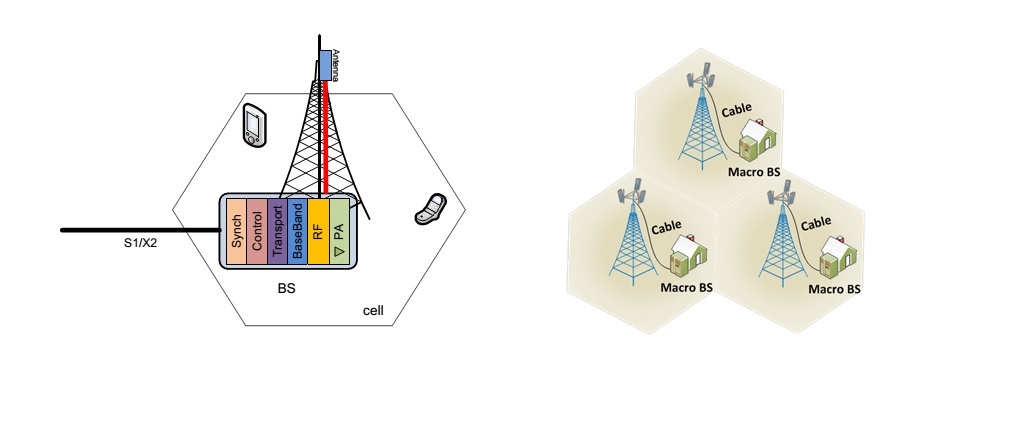
\includegraphics[scale=0.7]{./fig/c11}
  \caption{ساختار سنتی ایستگاه پایه \cite{checko2015cloud}}
  \label{fig:c11}
\end{figure}
هر ایستگاه پایه دو نوع پردازش انجام می دهد : پردازش
رادیویی که توسط واحد رادیویی \LTRfootnote{RRH} انجام می شود و شامل پردازش
دیجیتالی، فیلترینگ فرکانسی، تقویت توان و ....میباشد و
پردازش باند پایه که توسط واحد باند پایه \LTRfootnote{BBU} که همان واحد کنترل است \LTRfootnote{CU} انجام شده و از جمله
مهمترین وظایف آن می توان به کدینگ، مدولاسیون و
تبدیل فوریه ی سریع اشاره کرد. در ساختار جدیدی که
تحت عنوان \lr{C-RAN}  معرفی خواهیم نمود نحوه ی ارتباط
پردازشگرهای رادیویی و باند پایه متحول شده و در نتیجه
مزایایی برای شبکه حاصل خواهد شد.در ادامه ، انواع ساختارها را بیان خواهد شد.
\subsubsection{ساختار سنتی ایستگاه پایه }

در ساختارهای سنتی ایستگاه پایه، پردازش های رادیویی و باند پایه در
داخل ایستگاه پایه انجام می شد و مدول آنتن نیز در فاصله
ی چند متری از مدول رادیویی نصب شده و ارتباط آنها
توسط کابل کواکسیال برقرار می شد که همین امر سبب
افزایش تلفات در شبکه می باشد. این نوع ساختار در شکل
\ref{fig:c11} نشان داده شده است. همان گونه که مشاهده می کنید
ارتباط بین ایستگاههای پایه توسط ارتباط  $X_2$ و ارتباط بین
ایستگاه پایه و شبکه ی هسته توسط ارتباط $ S_1$ برقرار می
شود. این نوع ساختار در شبکه های \lr{1G} و \lr{2G} به کار گرفته
شده است 
\cite{checko2015cloud}.

%Figure \ref{fig:gull} shows a photograph of a gull.
\subsubsection{ ساختار ایستگاه پایه و واحد رادیویی}

\begin{figure}
  \centering
    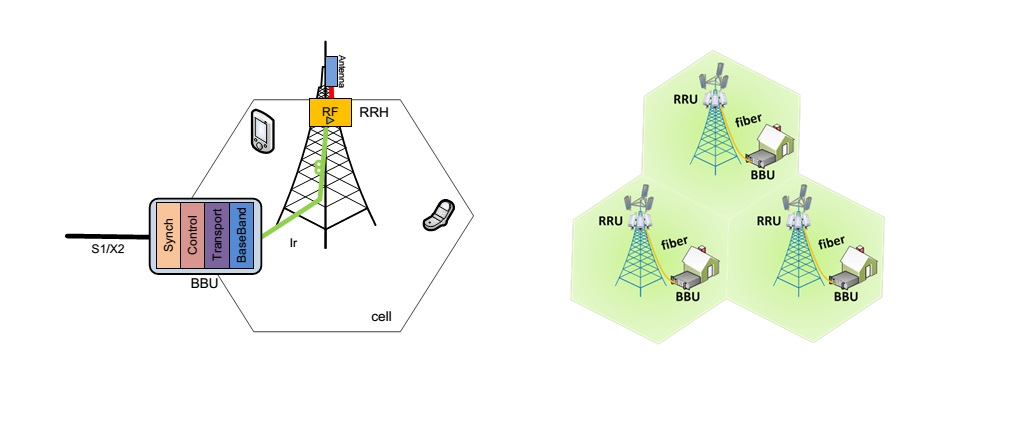
\includegraphics[scale=0.7]{./fig/c22}
  \caption{ ساختار ایستگاه پایه و واحد رادیویی \cite{checko2015cloud}}
  \label{fig:c22}
\end{figure}
در این ساختار واحد رادیویی و واحد پردازشی سیگنال، از هم
مجزا شده و واحد رادیویی که تحت عنوان \lr{RRH} یا \lr{RRU}
نیز شناخته می شود، توسط فیبر نوری به واحد باند پایه یا \lr{BBU} اتصال می
یابد. همان طور که پیشتر بیان شد واحد رادیویی مسئولیت
انجام پردازش های دیجیتالی از جمله تبدیل انالوگ به
دیجیتال، دیجیتال به انالوگ، تقویت توان و فیلترینگ رابر عهده دارد، که تفکیک وظایف واحد پردازشی و واحد
رادیویی در این ساختار در شکل \ref{fig:c22} قابل مشاهده است. این
نوع ساختار برای شبکه های نسل سوم معرفی شده و امروزه
نیز بیشتر ایستگاههای پایه از همین ساختار بهره می گیرند.
از جمله ویژگی های بارز این ساختار امکان ایجاد فاصله
بین واحد رادیویی و پردازشی می باشد، که این فاصله به
دلیل تاخیر پردازشی و انتشاری نمی تواند از  $40$کیلومتر
فراتر رود. در این ساختار تجهیزات مرتبط با \lr{BBU} می
توانند به مکانی مناسبتر که قابل دسترس تر بوده و هزینه
ی اجاره و نگهداری کمتری را به اپراتورها تحمیل می
کنند منتقل شوند و واحد های رادیویی نیز در در پشت بام
ساختمان ها و مکان های مرتفع نصب می شوند که این
خود سبب کاهش هزینه های خنک سازی ادوات موجود
می شود. نحوه ی ارتباط بین \lr{RRH} و \lr{BBU} مشابه ساختار
سنتی بوده و \lr{RRH} ها نیز توسط معماری زنجیروار با هم
در ارتباطند.
\begin{figure}[H]
  \centering
    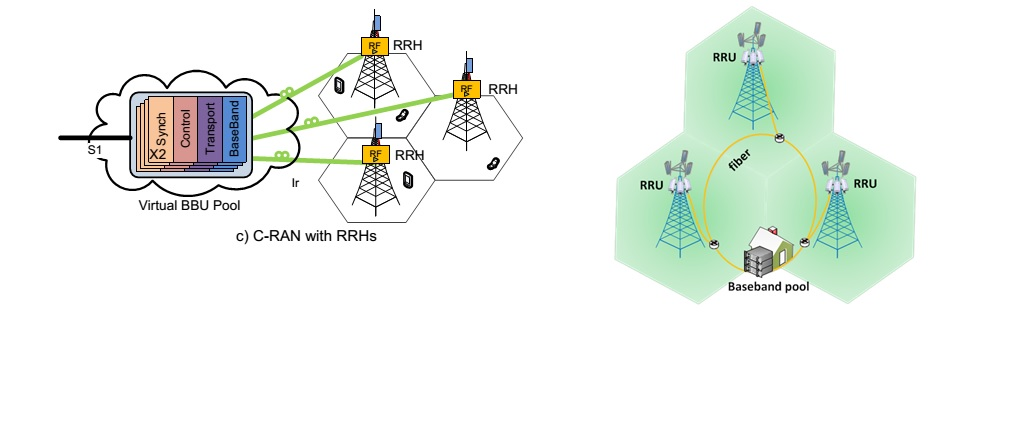
\includegraphics[scale=0.7]{./fig/c33}
  \caption{ساختار  \lr{C-RAN} \cite{checko2015cloud}}
  \label{fig:c33}
\end{figure}
\subsubsection{ساختار \lr{C-RAN}}
در ادامه ساختار های شبکه دسترسی رادیویی ابری و ساختارهای بهبود یافته ی آن را معرفی می نماییم.
\begin{itemize}
\item \textbf{شبکه های دسترسی رادیویی ابری}


ایده اصلی \lr{C-RAN} جداسازی بخش رادیویی (\lr{RRH}) 
\LTRfootnote{Radio Remote Head}
 از واحد پردازشی باند پایه (\lr{BBU})
 \LTRfootnote{Baseband Unit}
  است.
از تجمیع \lr{BBU} ها بر روی سرور ابری، \lr{BBU-Pool} ایجاد می شود.
در این ساختار، در راستای بهینه سازی عملکرد \lr{BBU}
 ها در مواجهه باایستگاههای پایه پر ترافیک و کم ترافیک،
 \lr{BBU}ها به صورت یک مجموعه ی واحد تحت عنوان 
\lr{BBU Pool}
 در آمده اند که این مجموعه بین چندین سلول 
 به اشتراک گزارده شده و مطابق شکل زیر مجازی سازی
می شود. 
در توضیح بیشتر این ساختار می توان این گونه
عنوان کرد که \lr{BBU Pool} به عنوان یک خوشه ی مجازی
در نظر گرفته می شود که شامل پردازش گرهایی می باشد
که پردازش های باند پایه را انجام می دهند. ارتباط بین
  \lr{BBU}ها در ساختار های فعلی به شکل  $X_2$ برقرار می شود
که در این ساختار ارتباط بین خوشه ها از فرم جدید $X_2$
تحت عنوان  $X_2 +$برقرار می شود.
\newline
در شکل \ref{fig:C-RAN} ساختار کلی شبکه ی  \lr{C-RAN} در سیستم های
\lr{ LTE}
 نمایش داده شده است. همان طور که در شکل قابل
مشاهده می باشد ساختار کلی شبکه  \lr{C-RAN} به دو بخش
 \lr{backhaul} و \lr{fronthaul} تقسیم بندی شده است. بخش
 \lr{fronthaul}شبکه به مرحله ی اتصال سایت های \lr{ RRH}به
 به \lr{BBU Pool} به اتصال \lr{backhaul} و بخش \lr{BBU Pool}
هسته ی شبکه ی سیار اطلاق می شود. همان گونه که قبلا
ذکر شد  \lr{ RRH}ها در نزدیکی انتن نصب شده و از طریق
لینک های انتقالی نوری با پهنای باند وسیع و تاخیر کم به
پردازشگرهای قوی در  \lr{BBU}متصل می شوند. توسط این
لینک های انتقالی است که سیگنال های دیجیتالی باند
پایه از نوع \lr{IQ} بین \lr{RRH} و \lr{BBU} انتقال می یابند \cite{checko2015cloud}.
\begin{figure}[H]
  \centering
    \includegraphics[width=\textwidth]{./fig/CRAN}
  \caption{ساختار شبکه ی \lr{C-RAN} \cite{checko2015cloud}}
  \label{fig:C-RAN}
\end{figure}
\item \textbf{شبکه های دسترسی رادیویی ابری نا متجانس (\lr{H-CRAN})}


برای غلبه بر چالش های شبکه های \lr{C-RAN} با محدودیت های \lr{fronthaul} ، شبکه های دسترسی ابری نامتحانس (\lr{H-CRAN}) معرفی می شود\cite{ fogComputing, heterogeneous, fogEdge}.
\begin{figure}
  \centering
    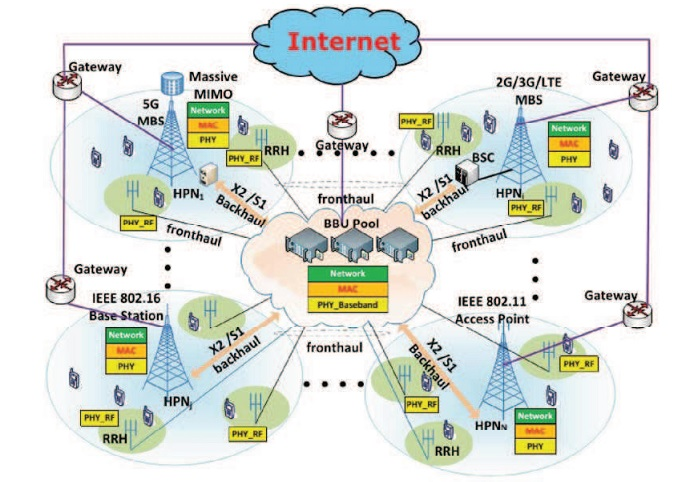
\includegraphics[scale = 0.8]{./fig/hc}
  \caption{ ساختار شبکه های دسترسی ابری نامتحانس \cite{heterogeneous}  }
  \label{fig:hc}
\end{figure}

کاربر و صفحه ی کنترلگر در چنین شبکه هایی از هم مجزا می باشند. که در این شبکه ها ، نودهای توان بالا   \LTRfootnote{High Power Node}\lr{HPN} ، عمدتا برای فراهم کردن پوشش بدون درز و اجرای عملکرد صفحه کنترل می باشد. در حالی که \lr{RRH} ها برای فراهم نمودن سرعت بالای نرخ داده برای انتقال بسته در ترافیک قرار گرفته اند. \lr{HPN} ها از طریق لینکهای \lr{backhaul}  به \lr{BBU Pool} متصلند ( برای هماهنگ کردن تداخل ).\newline
ساختار این شبکه شبیه به ساختار \lr{C-RAN} می باشد . همانطور که در شکل \eqref{fig:hc} نشان داده شده است ، تعداد زیادی \lr{RRH} ، همراه با انرژی مصرفی کم در ساختار \lr{H-CRAN} ، با یکدیگر در \lr{BBU Pool} مرکزی ، همکاری می کنند تا گین مشترک بالایی بدست آورند.   تنها ، فرکانس رادیویی جلو ،(\lr{RF}) و عملکردهای پردازشی  ساده ، در \lr{RRH} ، صورت می گیرد ، در حالی که پردازشهای مهم دیگر ، در \lr{BBU Pool} انجام می گیرد. همچنین تنها بخشی از عملکردها در لایه ی \lr{PHY} در \lr{RRH} به مشارکت می انجامد که این مدل در شکل \eqref{fig:hc} نشان داده شده است.\newline
اگرچه ، برخلاف \lr{C-RAN} ، \lr{BBU Pool} در \lr{H-CRAN} ، به \lr{HPN} ها متصلند که این، برای کاهش تداخل متقابل بین \lr{RRH} ها و \lr{HPN} ها از طریق محاسبات ابری متمرکز بر اساس تکنیکهای پردازشی مشترک می باشد. همچنین ، داده و واسط کنترل ، بین \lr{BBU Pool} و \lr{HPN} های $S_1$ و $X_2$ شناخته شده اند که تعریف آنها بر اساس تعریف استاندارد \lr{3G} ایجاد شده است.\newline
همانطور که سرویسهای صدا ، می توانند به صورت بهینه در طول مد سوییچ بسته در \lr{4G} فراهم گردند ، \lr{H-CRAN} می تواند به طور همزمان سرویس صدا و داده را پشتیبانی کند. سرویس صدا مرجح به اداره از طریق \lr{HPN} ها می باشد ، در حالی که ترافیک بسته ی پر داده ، بیشتر توسط \lr{RRH} اداره می گردد. 
در مقایسه با ساختار \lr{C-RAN} ،ساختار \lr{H-CRAN} ، نیازهای \lr{fronthaul} را بوسیله ی مشارکت \lr{HPN} ها برطرف می سازد. با توجه به حضور \lr{HPN} ها ،سیگنالهای کنترلی و سمبلهای داده در \lr{H-CRAN} جدا از هم می باشند. تمام کنترل کننده های سیگنال و سیستم هایی که اطلاعات را ارسال می نمایند ، توسط \lr{HPN} ها به \lr{UE} ، منتقل می گردد که منجر به سادگی در ظرفیت و در محدودیت تاخیر زمان در لینکهای \lr{fronthaul } بین \lr{RRH} ها و \lr{BBU Pool}  می گردد و منجر به صرفه جویی در مصرف انرژی می گردد. همچنین ، برخی از ترافیک های شدید و ناگهانی \LTRfootnote{Burst Traffic} و یا سرویس پیام همراه با مقدار داده ی کم ، می تواند به صورت بهینه توسط \lr{HPN} ها پشتیبانی گردد. مکانیزم کنترل بین ارتباط داشتن و نبود ارتباط ، توسط \lr{H-CRAN} پشتیبانی می گردد که منجر به حفظ کردن مقدار قابل توجهی \lr{Overhead} در رادیو بوسیله ی مکانیزم ارتباط جهت دار خالص می گردد. در \lr{RRH} ، تکنولوژی های مختلف انتقال در لایه ی \lr{PHY} ، قابل استفاده برای بهبود نرخ انتقال (همانند موج میلیمتری و نور مرئی) می گردد. در \lr{HPN}ها، \lr{MIMO}\LTRfootnote{Multiple Input Multiple Output}، یکی از راه های افزایش پوشش در بهبود ظرفیت می باشد.

\item \textbf{ساختار دسترسی رادیویی مهی}


برای حل کردن مشکلات \lr{H-CRAN} و \lr{C-RAN}، نیاز به معرفی ساختار جدید دیگری می باشیم که آن را \lr{F-RAN} می نامیم.
\lr{F-RAN} تمام ویژگی های مثبت محاسبات ابری و شبکه های نامتجانس و محاسبات مهی را همزمان در بر می گیرد.
محاسبات مهی ، اصطلاحی برای جایگزین کردن محاسبات ابری است که مقدار قابل توجهی از ذخیره سازی ، ارتباطات ، کنترل کردن ، اندازه گیری و مدیریت را در لبه ی شبکه انجام می دهد (نه در کانال و ابر مرکزی) \cite{fogComputing, fogEdge}.
 سیستمهای \lr{F-RAN} تحولی از سیستمهای \lr{C-RAN} می باشد . برخی از ارتباطات توزیع شده و عملکردهای ذخیره سازی در منطق لایه ی مه قرار دارد. همچنین چهار نوع ارتباطات ابری تعریف شده است.
  \begin{figure}[H]
  \centering
    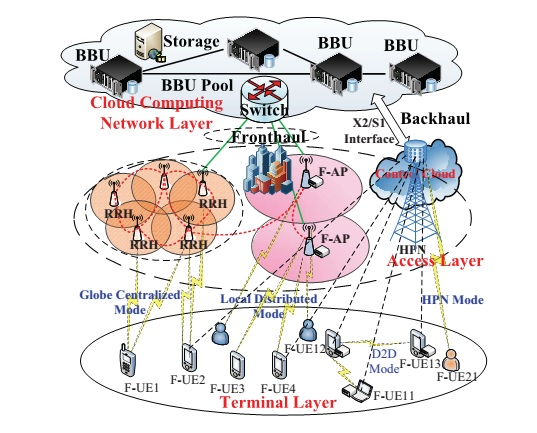
\includegraphics[scale =0.7]{./fig/fr}
  \caption{ مدل سیستم \lr{F-RAN} \cite{fogComputing} }
  \label{fig:fr}
\end{figure}
 \begin{itemize}
 \item
 ابر ذخیره گر و ارتباطات مرکزی جامع :
 که همانند ابر مرکزی \lr{C-RAN} می باشد
 \item
 ابر کنترل گر مرکزی :که برای تکمیل عملکردهای کنترلی  می باشد و در \lr{HPN} ها قرار دارد
 \item
 ابر ارتباطات منطقی توزیع شده که در برنامه های محاسبات مهی و ابزار های این محاسبات قرار دارد.
 \item
  ابر ذخیره گر منطق توزیع شده:
  که همانند قبل در \lr{F-RAN} قرار دارد.
 \end{itemize}
 در این ساختار ، برای کاهش تاخیر ناشی از انتقال داده ها به ابر مرکزی ، ساختار های \lr{RRH} را دارای حافظه قرار می دهیم که برای ارتباطات محلی، به جای اینکه پردازش ها در \lr{BBU Pool} صورت بگیرد، بدون نیاز به انتقال به ابر مرکزی، درون \lr{RRH} ها انجام پذیرد. 
\end{itemize}
\subsection{\lr{xRAN}}
\lr{xRAN}
در سال ۲۰۱۶ با هدف استانداردسازی یک جایگزین انعطاف پذیر و باز برای \lr{RAN}
مبتنی بر سخت افزار سنتی بدست آمده است.
 در این ساختار، سه حوزه ی مهم مورد بررسی قرار گرفته است.
اولین حوزه ی مورد بررسی، جداسازی بخش
صفحه ی کنترل
 \LTRfootnote{control plane} از 
 صفحه ی کاربر
\LTRfootnote{user plane}
می باشد. حوزه ی دوم،
ساختن یک پشته نرم افزاری \lr{eNodeB} مدولار که از سخت افزار \lr{COTS} استفاده می کند، می باشد.
حوزه ی سوم مورد بررسی، انتشار رابط های باز شمال و جنوب است\cite{xran}.
در ادامه این سه حوزه به طور دقیق تر مورد بررسی قرار می گیرد\cite{xran1}.

\begin{itemize}
\item \textbf{ جداسازی بخش صفحه ی کنترل از 
صفحه ی کاربر}:
این انتقال صفحه ی کنترل، که قبلاً کاملاً به دستگاههای سخت افزاری \lr{RAN} متصل بود، به دستگاههای محاسباتی در دسترس امکان می دهد \lr{RAN} بتواند به عنوان یک استخر منطقی از ظرفیت ، با کارایی بیشتری کار کند.
نرم افزار \lr{eNodeB} از سخت افزار خاص فروشنده جدا می شود و الهام بخش نوآوری در هر دو نرم افزار و سخت افزار به صورت مشارکتی اما به طور مستقل است.
برنامه نویسی و کنترل زمان واقعی بی سابقه در زیرساخت های \lr{RAN} به دست آمده است، که به راحتی از برنامه های کاربردی تلفن همراه و خدمات تجاری پشتیبانی می کند.
\item \textbf{ساختن یک پشته نرم افزاری \lr{eNodeB} مدولار}:
رویکرد \lr{xRAN} به خوبی با طرح های مجازی سازی عملکرد شبکه حامل \lr{(NFV)} مطابقت دارد، و همچنین منجر به کنترل عملکرد ترافیک با کارایی بالا، مدیریت تداخل و کنترل منابع رادیویی روی سیستم عامل های استاندارد \lr{x86} و می شود.
\item \textbf{انتشار رابط های باز شمال و جنوب}: 
رابط های استاندارد و باز قابیت پشتیبانی از فروشنده های متعدد همکاری اثبات شده دارند. 
\lr{xRAN.org}
و اعضای آن به تصویب رساندن این رابط ها از طریق فرآیندهای استاندارد منجر به در دسترس قرار دادن معماری \lr{xRAN} و پشتیبانی مورد نیاز می شوند.

\end{itemize}
\subsubsection{مزایای ساختار \lr{xRAN}}
\begin{itemize}
\item 
جداسازی بخش صفحه ی کنترل از 
صفحه ی کاربر 
منجر به 
برنامه ریزی زمان واقعی بی سابقه و کنترل در زیرساخت \lr{RAN} می شود که به راحتی برنامه های کاربردی تلفن همراه و خدمات تجاری را پشتیبانی می کند.
\item 
یک پشته \lr{eNB} مدولار مبتنی بر نرم افزار ، منجر به امکان قرارگیری انعطاف پذیر توابع \lr{eNB} و کنترل ترکیبی آن با یک برنامه ریز امکان پذیر می شود تا بتواند زمان تاخیر متغیر در \lr{fronthaul} را کنترل کند.
\item 
رابط های مرزی جنوبی استاندارد، پیاده سازی شبکه با خرید سیستم از چندین شرکت متفاوت را امکان پذیر می سازد و رابط های شمال مرزی، برش کامل شبکه برای بهینه سازی \lr{QoE} \LTRfootnote{Quality of Experience} کاربر را فراهم می کند.
رابط های \lr{xRAN} به خوبی با لبه ابر حامل هماهنگ هستند و اجازه می دهد تا  محاسبه و ذخیره سازی منابع در شبکه تلفن همراه 
به صورت دینامیکی مدیریت شود.
\item 
این ساختار هزینه ی رشد ظرفیت دسترسی رادیویی و هزینه ی بهره برداری را کاهش می دهد.
\end{itemize}
\subsection{\lr{ORAN}}
معماری \lr{ORAN} برای ایجاد زیرساخت های \lr{RAN} نسل بعدی طراحی شده است.
معماری \lr{ORAN} با تکیه بر اصول هوشمندی و باز بودن، پایه و اساس ساخت \lr{RAN} مجازی بر روی سخت افزار آزاد ، با کنترل رادیویی ایجاد شده توسط هوش مصنوعی است که توسط اپراتورهای سراسر جهان پیش بینی شده است.
این معماری بر روی رابط های استاندارد و تعریف شده ای بنا شده است تا یک زنجیره اکوسیستم با قابلیت باز ایجاد کند که دارای پشتیبانی کامل از استانداردهای تبلیغ شده توسط \lr{3GPP} و سایر سازمان های استاندارد صنعت فراهم شود.
\begin{figure}[H]
  \centering
    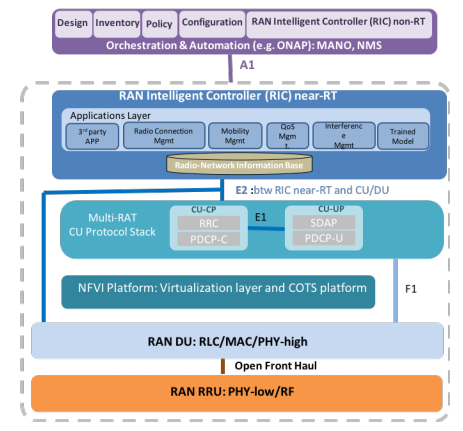
\includegraphics[width=0.8\textwidth]{./fig/oran1}
  \caption{ساختار شبکه ی \lr{ORAN} \cite{oranWP}}
  \label{fig:ORAN}
\end{figure}
اتحاد \lr{ORAN} در جستجوی چشم انداز باز بودن و هوشمندی برای شبکه های بی سیم نسل بعدی و فراتر از آن است\cite{oranWP}.
\begin{itemize}
\item \textbf{باز بودن}:
ایجاد یک \lr{RAN} مقرون به صرفه نیاز به باز بودن ارتباط ها دارد.
رابط های باز برای فعال کردن فروشندگان و اپراتورهای کوچکتر به سرعت می توانند خدمات خود را معرفی کنند و یا اپراتورها را قادر می سازد تا شبکه را متناسب با نیازهای منحصر به فرد خود تنظیم کنند.
رابط های باز همچنین استقرار چند سازنده ای را قادر می سازد و اکوسیستم تأمین کننده رقابتی تر و پر جنب و جوش بیشتری را ایجاد می کند.
 همچنین نرم افزارهای منبع باز و طرحهای مرجع سخت افزار باعث نوآوری سریعتر و دموکراتیک تر می شود.
 \item \textbf{هوشمندی}
 شبکه ها با ظهور برنامه 5G پیچیده تر و متراکم تر شده و خواستار برنامه های غنی تر می شوند.
 برای کاستن این پیچیدگی نمی توان از ابزارهای سنتی انسانی  برای استقرار، بهینه سازی و بهره برداری از شبکه استفاده کرد.
 در نتیجه، شبکه ها باید خود متحرک شوندتا بتوانند از فن آوری های جدید مبتنی بر یادگیری برای خودکارسازی عملکرد شبکه های عملیاتی و کاهش \lr{OPEX} استفاده کنند.
 اتحاد \lr{ORAN} تلاش خواهد کرد تا از تکنیک های یادگیری عمیق در حال ظهور استفاده کند تا بتواند هر لایه از معماری \lr{RAN}  را به طور هوشمند پیاده سازی کند.
 پیاده سای هوشمند هم در مولفه ها و خم در سطح شبکه اعمال می گردد و منجر به تخصیص دینامیکی منابع رادیویی و بهینه سازی بازدهی شبکه می گردد.
 همراه با رابط های باز \lr{ORAN}، اتوماسیون حلقه بسته بهینه شده با هوش مصنوعی دست یافتنی است و دوره جدیدی را برای عملیات شبکه امکان پذیر می کند.
\item \textbf{روش های هوش مصنوعی \lr{AI}
 \LTRfootnote{Artificial Intelligent}
  منجر به هوشمند سازی بخش رادیویی با استفاده از نرم افزار تعریف شده \LTRfootnote{Software Defined} 
  می شود:}
   مفهوم 
  \lr{SDN}
  \LTRfootnote{software defined network}
  که مبنی بر جداسازی 
   بخش صفحه ی کنترل \lr{CP} از
   صفحه ی کاربر 
\lr{UP}
می باشد، در ساختار 
\lr{ORAN}
مورد بررسی قرار می گیرد.
این جداسازی منجر به بهبود 
\lr{RRM}
برای استفاده از زمان غیر واقعی و زمان نزدیک به واقعی در کنترلگر هوشمند شبکه ی دسترسی رادیویی \LTRfootnote{RAN Intelligent Controller} \lr{RIC} 
با استفاده از رابط های 
\lr{A1}
و
\lr{E2}
 می گردد.
همچنین 
منجر به جداسازی 
 \lr{CU}
 از 
 \lr{CP/UP}
 می شود
 که از طریق رابط \lr{E1} در \lr{3GPP } توسعه می یابد.
\item \textbf{مجازی سازی بخش \lr{RAN}}:
 ابری سازی RAN یکی از اصول مهم ساختار 
 \lr{ORAN}
  می باشد.
 اپراتورها برای پشتیبانی از شکافهای مختلف در شبکه، الزامات NFVI/VIM را برای تقویت سیستم عامل مجازی ارائه می دهند.
 به عنوان مثال: لایه ی بالا بین PDCP و RLC تقسیم می شود و لایه ی پایین در PHY تقسیم می شود.
\item \textbf{رابط های باز}:
معماری مرجع ORAN بر روی مجموعه ای از رابط های کلیدی بین چندین جزء جدا شده ی RAN ساخته شده است.
اینها شامل رابط های \lr{3GPP} پیشرفته 
(
\lr{F1}،
\lr{W1}،
\lr{E1}،
\lr{X2}،
\lr{Xn}
)
 برای قابلیت همکاری بین چندین شرکت مختلف تولید کننده است.
رابط های مشخص شده \lr{ORAN Alliance} شامل یک رابط fronthaul باز بین DU و RRU ، رابط \lr{E2} و یک رابط \lr{A1} بین لایه 
Orchestration/NMS 
است که شامل عملکرد
 غیر واقعی زمانی \LTRfootnote{non real time RIC} و عملکرد eNB / gNB حاوی عملکرد RIC نزدیک به زمان واقعی 
\LTRfootnote{near-real time RIC} 
است.
\item \textbf{سخت افزار جعبه سفید}:
برای بهره مندی کامل از مقیاسی از اقتصاد ارائه شده توسط یک رویکرد  محاسباتی باز، \lr{O-RAN Alliance } 
طرح های مرجع 
سخت افزاری و ایستگاه پایه به صورت جعبه سفید با کارایی بالا را مشخص می کند. 
سیستم عامل های مرجع از یک رویکرد جدا شده پشتیبانی می کنند و نقشه های مفصلی را برای معماری سخت افزار و نرم افزار ارائه می دهند تا هم BBU و RRU را فعال کنند. 
\item \textbf{نرم افزار منبع باز}:
اتحادیه ORAN ارزش انجمن هایی که منابع باز ارا‌ئه می دهند را درک کرده   
 و از آنها پشتیبانی می کند.
 بسیاری از مؤلفه های معماری ORAN به صورت منبع باز از طریق جوامع موجود تحویل داده می شود.
 این مؤلفه ها عبارتند از: کنترلر هوشمند RAN ، پشته پروتکل ، پردازش لایه PHY و بستر مجازی سازی.
  چارچوب نرم افزار منبع باز ORAN نه تنها رابط های 
(
\lr{F1}،
\lr{W1}،
\lr{E1}،
\lr{E2}،
\lr{X2}،
\lr{Xn}
)
  را پیاده سازی می کند ، بلکه انتظار دارد که طراحی مرجع را برای نسل بعدی RRM با هوش جاسازی شده ارائه دهد تا RIC را امکان پذیر کند.
\end{itemize}

\lr{ORAN}،
 المانهای شبکه ی دسترسی رادیویی را مجازی می کند، آنها را جدا کرده و رابط های باز مناسب را 
برای اتصال این عناصر
تعیین می کند. همچنین، 
\lr{ORAN}
از روشهای یادگیری ماشین برای هوشمندسازی لایه های 
\lr{RAN}
 استفاده می نماید. 
 در ساختار نوآورانه ی 
 \lr{ORAN}
 نرم افزار قابل برنامه ریزی 
 \lr{RAN}
 از سخت افزار جدا می شود.
  یکی از مهم ترین خصوصیات
  \lr{ORAN}
  رابط کاربری باز است که به اپراتورهای موبایل این قابلیت را می دهد تا بتوانند سرویس های مورد نیاز خود را تعریف نمایند.

در ساختار
\lr{ORAN}،
واحد توزیع شده \lr{DU}،
نود منطقی می باشد که شامل لایه های 
\lr{RLC}
،
\lr{MAC}،
و
\lr{High-PHY}
است.
علاوه بر این، واحد مرکزی 
\lr{CU}
نود منطقی است که شامل لایه های 
\lr{RRC}،
\lr{SDAP} 
و 
\lr{PDCP}
می باشد.
نود منطقی واحد رادیویی
\lr{RU}
نیز، شامل لایه ی 
\lr{LOW-PHY}
و بخش پردازش رادیویی می باشد.
\lr{ORAN}
،
رابطهایی از جمله رابط 
\lr{fronthaul}
باز را شامل می شود که بخش \lr{DU} را به \lr{RU} متصل می نماید
(رابط 
\lr{E2}). 
همچنین
 رابط \lr{A1}
 بین لایه ی 
  \lr{orchestration/NMS}
  که شامل 
  تابع غیر واقعی زمان است و 
  \lr{eNB/qNB}
  که شامل تابع نزدیک به زمان است. 


  با افزایش ترافیک تلفن همراه، شبکه های تلفن همراه و تجهیزاتی که آنها را اجرا می کند باید نرم افزاری تر ، مجازی، انعطاف پذیر، هوشمند و کارآمدتر شوند.
اتحادیه ی ORAN متعهد است در حال تکامل شبکه های دسترسی رادیویی باشد که باعث می شود آنها نسبت به نسلهای قبل بازتر و باهوش تر شوند.
تجزیه و تحلیل در زمان واقعی که توسط سیستم های یادگیری ماشین تعبیه شده است و ماژول های پایانی هوش مصنوعی را هدایت می کند، باعث تقویت هوش شبکه می شود.
عناصر شبکه مجازی با رابط های باز و استاندارد، جنبه های اصلی طرح های مرجع توسعه یافته توسط اتحادیه ی ORAN خواهد بود.
فن آوری های موجود از عناصر شبکه منبع باز و جعبه سفید، نرم افزار و اجزای سخت افزاری مهم این طرح های مرجع خواهد بود.
\section{مجازی سازی توابع شبکه}
برای بهبود سرویس دهی در نسل پنجم مخابرات، جداسازی المان های نرم افزاری و سخت افزاری شبکه صورت گرفته است و به عنوان 
مجازی سازی توابع شبکه (\lr{NFV}) \LTRfootnote{network function virtualization}
معرفی شده است.
  حال توابع شبکه ی مجازی
  \lr{VNF}
  \LTRfootnote{Virtual network function} ،
  بلوکهای توابع سیستم هستند.
در نسل پنجم مخابرات 
  انتظار می رود که
   میزبان چندین سرویس
   با نیازهای مختلف به طور همزمان
    باشند.
    ایده اصلی NFV جداسازی تجهیزات شبکه فیزیکی از توابع اجرا شده بر روی آنها است. این بدان معنی است که یک عملکرد شبکه - مانند فایروال - می تواند به عنوان نمونه ای از نرم افزارهای ساده به فراهم آورندگان سرویس (SP) \LTRfootnote{Service Provider} ارسال شود.
    این امر امکان ادغام بسیاری از انواع تجهیزات شبکه بر روی سرورهای با حجم بالا ، سوئیچ ها و انبارها را فراهم می کند ، که می توانند در مراکز داده، نودهای شبکه توزیع شده و در محل کاربر نهایی قرار بگیرند.
    به این ترتیب، یک سرویس خاص می تواند به مجموعه ای از توابع شبکه مجازی (VNFs) تجزیه شود، که می تواند در نرم افزارهایی که روی یک یا چند سرور فیزیکی استاندارد در صنعت قرار دارند، اجرا شود.
    سپس VNF ها ممکن است در مکانهای مختلف شبکه (به عنوان مثال، با هدف معرفی خدمات هدفمند به مشتریان در یک موقعیت جغرافیایی خاص) جابجا شده و خدمات رسانی کنند، بدون اینکه لزوماً به خرید و نصب سخت افزار جدید نیاز داشته باشند.
    NFV به 
     هاSP
   با انعطاف پذیری بیشتری وعده می دهد تا بتواند بیشتر قابلیت ها و خدمات شبکه خود را به کاربران و سایر خدمات باز کنند و امکان استقرار یا پشتیبانی از سرویس های جدید شبکه را  به طور سریعتر و ارزانتر داشته باشند تا بتوانند  سرویس بهتری داشته باشند.
   برای دستیابی به این مزایا، NFV مسیر را برای کاهش اختلافات در نحوه ارائه خدمات شبکه در مقایسه با عملکرد فعلی ایجاد می کند. خلاصه این ویژگی ها به شرح زیر است
   \cite{NFV}.
 \begin{itemize}
  \item \textbf{جدا سازی بخش نرم افزار از سخت افزار}:
از آنجا که عنصر شبکه، ترکیبی از سخت افزارها و نرم افزارهای یکپارچه نخواهد بود، تکامل هر دو مستقل از یکدیگر می باشد.
که این ویژگی منجر به جداسازی زمان بندی توسعه و نگهداری نرم افزار و سخت افزار می گردد.
\item \textbf{استقرار عملکرد شبکه انعطاف پذیر:}
جدا کردن نرم افزار از سخت افزار به تنظیم مجدد و به اشتراک گذاری منابع زیرساختی کمک می کند،
بنابراین، سخت افزار و نرم افزار، باهمدیگر
می توانند در زمان های مختلف عملکردهای مختلفی را انجام دهد که به اپراتورهای شبکه کمک می کند تا خدمات جدید شبکه را سریعتر در همان پلت فرم فیزیکی مستقر کنند.
بنابراین،
مؤلفه ها را می توان در هر دستگاه با قابلیت NFV در شبکه قرار داد و اتصالات آنها به روشی انعطاف پذیر تنظیم کرد.
\item \textbf{مقیاس گذاری پویا}:
  جداشدن عملکرد شبکه به اجزای نرم افزاری  نعطاف پذیری بیشتری را برای  عملکرد واقعی VNF به روشی پویاتر، 
   با توجه به ترافیک واقعی که اپراتور شبکه برای تأمین ظرفیت نیاز دارد،
  فراهم می کند.
\end{itemize}  
 \subsection{ساختار شبکه }
 VNF
 ها برای به اشتراک گذاشتن منابع مختلف فیزیکی و مجازی زیرساخت ها می توانند مستقر و مجدداً تنظیم شوند ، تا مقیاس پذیری و کارآمدی سیستم را تضمین کنند که منجر می شود SP ها به سرعت سرویس های جدید را در سیستم وارد کنند.
 به طور کلی ، سه مؤلفه اصلی در NFV وجود دارد:
 خدمات ، NFVI و مدیریت NFV و orchestration
 \LTRfootnote{NFV-MANO}
 که در شکل \eqref{fig:NFV} دیده می شود.
 \begin{figure}
  \centering
    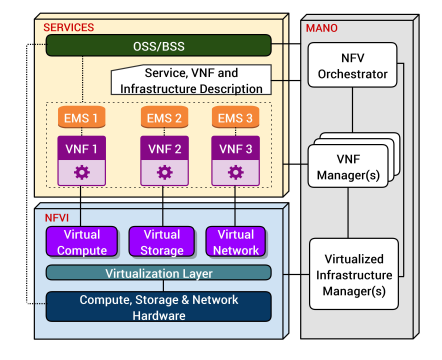
\includegraphics[width=0.8\textwidth]{./fig/NFV}
  \caption{ساختار NFV \cite{NFVArch}}
  \label{fig:NFV}
\end{figure} 
این مؤلفه ها به شرح زیر بیان می گردد\cite{NFVArch}.
\begin{enumerate}
\item 
خدمات: یک سرویس مجموعه ای از VNF ها است که می توانند در یک یا چند ماشین مجازی پیاده سازی شوند.
در بعضی مواقع ، VNF ها می توانند در ماشینهای مجازی نصب شده در سیستم عامل یا سخت افزار بطور مستقیم نصب شوند. آنها توسط سرپرستان بومی یا مانیتورهای ماشین مجازی اداره می شوند.
معمولاً توسط یک سیستم مدیریت عناصر \LTRfootnote{Element Management System} (EMS)،
 که مسئولیت ایجاد، تنظیمات، نظارت، عملکرد و امنیت آن است، اداره می شود.
 EMS 
 اطلاعات ضروری مورد نیاز سیستم پشتیبانی عملیات \LTRfootnote{Operations Support System}(OSS) را در یک محیط SP فراهم می کند.
 OSS
  سیستم مدیریت عمومی است، که  همراه با سیستم پشتیبانی از تجارت 
\LTRfootnote{Business Support System}  
  (BSS)
  ، به ارائه دهندگان کمک می کند تا چندین سرویس ارتباطی از راه دور را به کار ببندند و مدیریت کنند.
  (به عنوان مثال سفارش ، صورتحساب ، تمدید ، عیب یابی مشکل و غیره).
مشخصات NFV بر ادغام با راه حل های موجود OSS / BSS متمرکز است.
\item NFVI
:
زیرساخت های NFV تمام منابع سخت افزاری و نرم افزاری را که شامل محیط NFV است ، پوشش می دهد.
NFVI شامل اتصال شبکه بین مکان ها ، به عنوان مثال ، بین
مراکز داده و ابرهای ترکیبی عمومی یا خصوصی است.
منابع فیزیکی به طور معمول شامل محاسبات، ذخیره سازی و سخت افزار شبکه است که وظیفه ی آن پردازش، ذخیره سازی و اتصال VNF ها از طریق لایه مجازی سازی است و دقیقاً بالای سخت افزار قرار دارد و منابع فیزیکی را چکیده می کند (که به صورت منطقی تقسیم شده و به VNF ها اختصاص می یابد).
هیچ راه حل خاصی برای استقرار NFV وجود ندارد. در عوض معماری NFV می تواند از یک لایه مجازی سازی موجود مانند Hypervisor با ویژگی های استاندارد که منابع سخت افزاری را به راحتی استخراج می کند و آنها را به VNF ها اختصاص می دهد ، استفاده کند.
وقتی این پشتیبانی در دسترس نباشد ، اغلب ، لایه مجازی سازی از طریق یک سیستم عامل حاصل می شود که نرم افزاری را در بالای سرور غیر مجازی یا با اجرای یک VNF به عنوان یک برنامه اضافه می کند.
\item NFV-MANO
:
NFV-MANO
 از این موارد تشکیل شده است:
 orchestrator
 ،
 مدیران VNFs و مدیران زیرساخت مجازی.
 چنین بلوکی عملکردهای مورد نیاز برای کارهای مدیریتی را که برای VNF ها اعمال می شود، به عنوان مثال تهیه و پیکربندی را  ارائه می دهد. 
 NFV-MANO شامل orchestration و مدیریت چرخه منابع فیزیکی یا مجازی است که از مجازی سازی زیرساخت ها و مدیریت چرخه VNF ها پشتیبانی می کند.
 همچنین شامل بانکهای اطلاعاتی است که برای ذخیره اطلاعات و مدل های داده استفاده می شود که ویژگی های چرخه عمر توابع، خدمات و منابع را تعریف می کند.
 NFV-MANO روی کلیه وظایف مدیریتی مجازی سازی ویژه لازم در چارچوب NFV تمرکز دارد.
 علاوه بر این ، این چارچوب رابط هایی را تعیین می کند که می توانند برای ارتباطات بین مؤلفه های مختلف
  NFV MANO، 
 و همچنین هماهنگی با سیستم های سنتی مدیریت شبکه (یعنی OSS و BSS) مورد استفاده قرار گیرند تا امکان عملکرد هر دو VNF و کارکردهای اجرا شده بر روی تجهیزات فراهم شود.
 به طور خلاصه، اگر برش شبکه با استفاده از فایروال و DPI مستقر شده باشد، آنگاه NFV-MANO وظیفه دارد بگوید این VNF ها در کجای شبکه فیزیکی قرار دارند. همچنین این VNF ها توسط EMS و همان MANO کنترل می شوند.
\end{enumerate}
\section{شبکه تعریف شده نرم افزار (SDN)}
بنیاد شبکه باز 
\LTRfootnote{Open Networking Foundation}
(ONF) 
یک مجموعه ای است که به توسعه، استاندارد سازی و تجاری سازی SDN 
\LTRfootnote{Software Defined Network} 
پرداخت.
ONF
 به طور صریح و دقیق SDN را بدین صورت تعریف کرد:
 شبکه تعریف شده توسط نرم افزار (SDN) یک معماری شبکه است که کنترل شبکه از ارسال جدا می شود و به طور مستقیم قابل برنامه ریزی است.
 SDN توسط دو ویژگی تعریف می شود ، یعنی جدا شدن صفحه ی کنترل و داده و قابلیت برنامه ریزی در صفحه کنترل.
 با این وجود ، هیچ یک از این دو امضای SDN در معماری شبکه کاملاً جدید نیستند
 \cite{SDN1}.
 SDN 
 در اصل یک الگوی شبکه سازی متمرکز است که در آن هوش شبکه (یعنی عملکرد کنترل یا صفحه کنترل) به طور منطقی در یک یا مجموعه ای از موجودیت های کنترل (یعنی کنترل کننده های SDN) متمرکز می شود در حالی که صفحه ی انتقال داده،  ساده و چکیده شده برای برنامه های کاربردی می باشد و سرویس های شبکه درخواست خود را از طریق کنترل کننده های SDN
 بیان می کنند.
 در حالی که در مورد هسته اصلی شبکه موبایل LTE ، EPC صحبت می کنیم ، مفهوم SDN برای دستیابی به جدایی واضح بین صفحات کنترل و کاربر در اشخاص SGW و PGW استفاده می شود.
 با تقسیم دروازه به این روش (یعنی از SGW به SGW-C و
SGW-U 
و از PGW به PGW-C و (PGW-U 
  مقیاس بندی این مؤلفه ها به طور مستقل امکان پذیر است و طیف وسیعی از گزینه های استقرار را نیز ممکن می کند.
  
 پروتکل مورد استفاده بین صفحه ی کنترل و صفحه ی کاربر می تواند یا افزونه پروتکل موجود OpenFlow باشد، که توسط گروه کاری بی سیم و موبایل ONF (WMWG)با رابط های جدید، یعنی Sxa و Sxb ساخته می شود، که توسط  \lr{3GPP CUPS} تعریف و مشخص می شوند\cite{SDN2}. 
 جداسازی صفحه ی کنترل از کاربر منجر به کنترل بیشتر شبکه بوسیله ی برنامه می گردد که منجر به بهبود تنظیمات و کارآمدی سیستم می گردد.
 SDN
  با ساختار برنامه ریزی شده ی قوانین ترافیک، جایگزین امیدوار کننده ای برای فرماندهی ترافیک ارائه می دهد.
  ساختار SDN در شکل \eqref{fig:SDN} آورده شده است.
  \begin{figure}
  \centering
    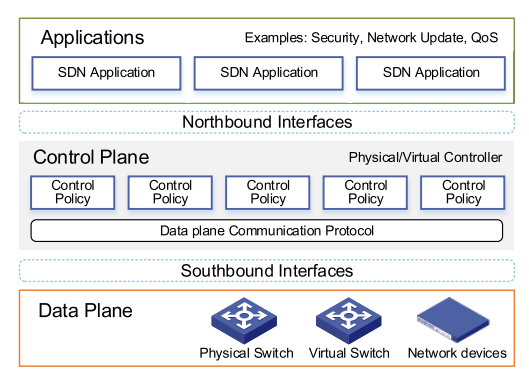
\includegraphics[width=0.8\textwidth]{./fig/SDN}
  \caption{ ساختار SDN \cite{SDN3}}
  \label{fig:SDN}
\end{figure} 
  در این ساختار ۳ لایه ی مختلف وجود دارد که در ادمه بیان می کنیم\cite{SDN3}.
  \begin{enumerate}
  \item لایه ی برنامه :
  این لایه مجموعه ای از برنامه های متمرکز بر خدمات شبکه را پوشش می دهد و آنها عمدتا برنامه های نرم افزاری هستند که با لایه کنترل ارتباط برقرار می کنند.
  \item لایه ی کنترل:
  به عنوان هسته اصلی SDN ، لایه کنترل از یک کنترلر متمرکز تشکیل شده است که منطقاً نمای شبکه جهانی و پویا را حفظ می کند ،  که از لایه برنامه درخواست می کند و دستگاه های شبکه را از طریق پروتکل های استاندارد مدیریت می کند.
  \item لایه ی داده:
  این لایه، زیرساخت ها شامل سوئیچ ها، روترها و لوازم شبکه می باشد. در زمینه SDN ، این دستگاه ها قابل برنامه ریزی هستند و از رابط های استاندارد پشتیبانی می کنند.
  \end{enumerate}
 \section{برش شبکه}
 پیش بینی می شود شبکه های \lr{5G} چندین سرویس را با نیازهای مختلف به طور همزمان پشتیبانی کند.
 برش شبکه
 \LTRfootnote{Network Slicing}
به عنوان راه حلی برای چنین تقاضا در نظر گرفته شده است.
یک برش شبکه، یک شبکه منطقی \lr{end-to-end} است که خدمات  با نیازهای خاص را ارائه می دهد.
 چندین برش شبکه
در یک زیرساخت یکسان
  اجرا و مدیریت می شوند و
به طور مستقل کار می کنند.
برش شبکه
 با هدف تقسیم منطقی مجموعه توابع و منابع شبکه در یک نهاد شبکه در نظر گرفته شده است که مطابق با خواسته های فنی یا تجاری خاص می باشد.
 با خرد کردن یک شبکه فیزیکی به چندین شبکه منطقی، برش شبکه می تواند از خدمات متناسب با تقاضا برای سناریوهای برنامه مشخص در همان زمان با استفاده از همان شبکه فیزیکی پشتیبانی کند.
با استفاده از برش شبکه، منابع شبکه می توانند به صورت پویا و کارآمد به برش های شبکه منطقی با توجه به خواسته های QoS مربوطه اختصاص داده شوند\cite{NS1}. 

\begin{figure}
  \centering
    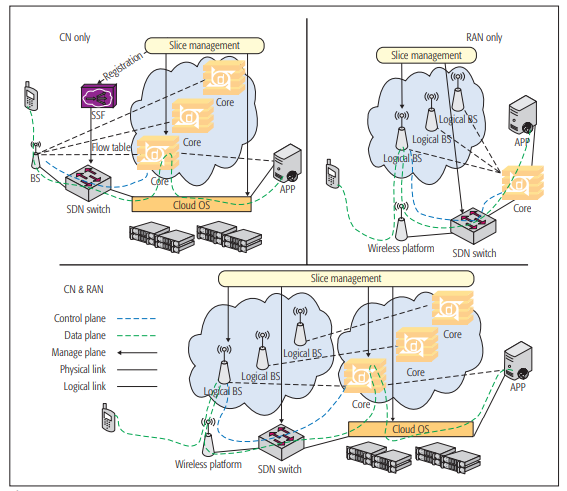
\includegraphics[width=0.8\textwidth]{./fig/NS}
  \caption{سه ساختار برش شبکه \cite{NS2}}
  \label{fig:NS}
\end{figure} 
پیاده سازی های مختلفی از برش شبکه وجود دارد که شامل برش هسته ی شبکه، برش \lr{RAN} و برش هر دو بخش می باشد\cite{NS2}.
\begin{itemize}
\item \textbf{برش هسته:}
هسته ی شبکه (CN) \LTRfootnote{core network}
به عنوان برش های شبکه، مجازی سازی می شوند که با ویژگی هایی مانند ویژگی های قابل برنامه ریزی و قابل اعتماد بودن که شامل مدیریت حرکت و تأیید اعتبار می باشد.
برش های شبکه فقط در CN وجود دارد.
  بنابراین، نه RAN و نه تجهیزات کاربر (UE) برای CNهای برش داده شده نیاز به تنظیم ویژه ندارند.
  در برش هسته ی شبکه، برش تنها در بخش هسته ی شبکه است و تمام واسط ها و فرآیندها، بدون تغییر باقی می مانند
  به جز مواردی که در ابتدا UE ها به شبکه ها وصل می شوند ، زیرا UE ها باید به برش صحیح CN ها اختصاص داده شوند.
\item \textbf{
برش شبکه ی دسترسی رادیویی:
}
برخلاف برش CN،
برش های RAN روی سخت افزار رادیویی و استخر منابع باند پایه، به نام یک سطح بی سیم، اجرا می شوند که دارای کشش کمتری نسبت به زیرساخت مجازی بالغ شده در CNها هستند.
با چند BS منطقی، برش های RAN پارامترهای مختلفی از رابط های هوا (به عنوان مثال ، طول نماد ، فاصله زیر حامل ، طول پیشوند چرخه و پارامترهای درخواست تکرار خودکار هیبریدی \LTRfootnote{HARQ}) را اعمال می کند.
علاوه بر این، پارامترهای دیگری مانند انتخاب سلول و آستانه انتقال، و همچنین سیاست های انتقال هماهنگ را می توان برای هر برش تعریف کرد تا یک تجربه بی سیم برجسته را به کاربران ارائه دهد.
\item \textbf{برش هسته و شبکه ی دسترسی رادیویی}:
در این سناریو، هر برش از RAN به یک برش از هسته متصل می شود، بنابراین اپراتورها می توانند یک شبکه منطقی انتهای به مشتریان ارائه دهند.
روش انتخاب برش همان روش برش RAN است، بنابراین کاربران پس از دسترسی به سیستم، نیازی به انتخاب برش CN ندارند.
این مدل از برش مزایای هر دو مدل از برش را باهم دارد.
 در نتیجه این روش برش، قادر به برنامه ریزی ویژگی های CN و همچنین دارای قابلیت تغییر رابط های هوایی RAN
 می باشد.
 
\end{itemize}
\section{نتیجه گیری}
  در این فصل ابتدا مروری بر تاریخچه ی مخابرات و ۵ نسل مخابراتی شد. سپس ساختار های مختف دسترسی رادیویی به طور خلاصه بیان شد و در نتیجه ی آن ساختار CRAN که ساختار ابری است تعریف شد. سپس ساختار xRAN
  مورد توجه قرار گرفت و در نهایت ساختار ORAN 
  که ترکیب و تکاملی از CRAN و xRAN می باشد مورد توجه قرار گرفت.
  
 بعد از بیان ساختارهای رادیویی، ساختار هسته ی شبکه را در نسل پنجم بیان کردیم که شامل 
 NFV و SDN 
 می باشد که منجر به جداسازی صفحه ی کنترل از کاربر می شود و سیستم هوشمندتر همراه با قابلیت برنامه ریزی بیشتر می گردد.
 در ادامه برش شبکه در بخش رادیویی و هسته و هردو مورد توجه قرار گرفته شد.
\section{خلاصه ای از فصل های آتی}
در فصل دوم مروری بر ادبیات پیشین و خلاصه ای از مدل سیستم مقالات موجود، بیان می گردد.
در فصل سوم مدل سیستم در نظر گرفته بیان می شود و صورت مسئله به نمایش گذاشته می شود و روش های حل آن بیان می گردد.
در فصل چهارم نتایج شبیه سازی قرار داده می شود.
در فصل پنجم نیز نتیجه گیری و کارهای آتی مورد نظر بیان می شود.   
 		% فصل اول: مقدمه
% !TeX root=../main.tex
\chapter{مروری بر مطالعات انجام شده}
%\thispagestyle{empty} 
\section{مقدمه}
هدف از این فصل که با عنوان‌های  «مروری بر ادبیات موضوع%
\LTRfootnote{Literature Review}»،
«مروری بر منابع» و یا «مروری بر پیشینه تحقیق%
\LTRfootnote{Background Research}»
معرفی می‌شود، بررسی و طبقه‌بندی یافته‌های تحقیقات دیگر محققان در سطح دنیا و تعیین و شناسایی خلأهای تحقیقاتی است. آنچه را که تحقیق شما به دانش موجود اضافه می‌کند، مشخص کنید. طرح پیشینه تحقیق%
\LTRfootnote{Background Information}
یک مرور محققانه است و تا آنجا باید پیش برود که پیش‌زمینهٔ تاریخی مناسبی از تحقیق را بیان کند و جایگاه تحقیق فعلی را در میان آثار پیشین نشان دهد. برای این منظور منابع مرتبط با تحقیق را بررسی کنید، البته نه آنچنان گسترده که کل پیشینه تاریخی بحث را در برگیرد. برای نوشتن این بخش:
\begin{itemize}
	\item
	دانستنی‌های موجود و پیش‌زمینهٔ تاریخی و وضعیت کنونی موضوع را چنان بیان کنید که خواننده بدون مراجعه به منابع پیشین، نتایج حاصل از مطالعات قبلی را درک و ارزیابی کند.
	\item
	نشان دهید که بر موضوع احاطه دارید. پرسش تحقیق را همراه بحث و جدل‌ها و مسائل مطرح شده بیان کنید و مهم‌ترین تحقیق‌های انجام شده در این زمینه را معرفی نمائید.
	\item
	ابتدا مطالب عمومی‌تر و سپس پژوهش‌های مشابه با کار خود را معرفی کرده و نشان دهید که تحقیق شما از چه جنبه‌ای با کار دیگران تشابه یا تفاوت دارد.
	\item
	اگر کارهای قبلی را خلاصه کرده‌اید، از پرداختن به جزئیات غیرضروری بپرهیزید. در عوض، بر یافته‌ها و مسائل روش‌شناختی مرتبط و نتایج اصلی تأکید کنید و اگر بررسی‌ها و منابع مروری عمومی دربارهٔ موضوع موجود است، خواننده را به آنها ارجاع دهید.
\end{itemize}

\section{تعاریف، اصول و مبانی نظری}
این قسمت ارائهٔ خلاصه‌ای از دانش کلاسیک موضوع است. این بخش الزامی نیست و بستگی به نظر استاد راهنما دارد.

\section{مروری بر ادبیات موضوع}
در این قسمت باید به کارهای مشابه دیگران در گذشته اشاره کرد و وزن بیشتر این قسمت بهتر است به مقالات ژورنالی سال‌های اخیر (۲ تا ۳ سال) تخصیص داده شود. به نتایج کارهای دیگران با ذکر دقیق مراجع باید اشاره شده و جایگاه و تفاوت تحقیق شما نیز با کارهای دیگران مشخص شود. استفاده از مقالات ژورنال‌های معتبر در دو یا سه سال اخیر، می‌تواند به اعتبار کار شما بیافزاید.

\section{نتیجه‌گیری}
‌در نتیجه‌گیری آخر این فصل، با توجه به بررسی انجام شده بر روی مراجع تحقیق، بخش‌های قابل گسترش و تحقیق در آن حیطه و چشم‌اندازهای تحقیق مورد بررسی قرار می‌گیرند.	در برخی از تحقیقات، نتیجه نهایی فصل روش تحقیق، ارائهٔ یک چارچوب کار تحقیقی 
\lr{(research framework)}
است.		% فصول دوم: مروری بر مطالعات انجام شده
\chapter{تخصیص منابع در شبکه‌های دسترسی رادیویی باز}
\section{مقدمه}
در این فصل، هدف تخصیص منابع در شبکه های \lr{Open RAN} در لینک فروسو می‌باشد که شامل تخصیص توان و برش های شبکه است.
در این بخش فرض بر این است که در شبکه ی نسل پنجم مخابرات از زیرساخت \lr{Open RAN} استفاده شده است. این شبکه سرویس هایی از قبیل \lr{IoT}، سرویس تلفن، پیامک و ... در اختیار کاربران قرار می‌دهد. در اینجا  مفهوم برش شبکه در سیستم بدین صورت به کار رفته که به جای دیدن کاربران به صورت مجزا، کاربرانی که از یک سرویس خاص استفاده می‌نمایند در دسته ی آن سرویس قرار گرفته و دسته بندی می‌شوند. همچنین برش هایی از شبکه در اختیار کاربران هر سرویس خاص، قرار می‌گیرد که هر برش شبکه شامل تعدادی واحد رادیویی
\LTRfootnote{Radio Unit}
(\lr{RU}) 
،
بلوک های منبع فیزیکی
 \LTRfootnote{Physical Resource Block}
 (\lr{PRB})، 
 یک واحد توزیع شده
\LTRfootnote{Distributed Unit}
(\lr{DU}) 
 ، 
 یک واحد مرکزی
\LTRfootnote{Centralized Unit}
(\lr{CU})  
  می‌باشد که هر واحد توزیع شده و مرکزی شامل تعدادی توابع شبکه ی مجازی شده
  \LTRfootnote{Virtual Network Function}
(\lr{VNF}) 
می‌باشد. 

در این سیستم هدف، بررسی مسئله ی برش شبکه در بخش RAN و بخشی از هسته در شبکه های دسترسی باز
ORAN
می‌باشد.
ما مسئله زمانبندی لینک بی سیم، اختصاص برشها به سرویسها و اختصاص مراکز داده به برشها را که از مشکلات بسته بندی جعبه  ۳-بعدی است را فرموله می‌کنیم. 
هدف این است که به طور مشترک بهره وری انرژی را به حداکثر برسانیم و مصرف توان واحدهای رادیویی را کاهش داده تا هزینه منابع فیزیکی را در یک کانال فروسو به حداقل برسانیم.
این مسئله به صورت یک مسئله ی 
mixed-integer
بیان می‌شود و به دو مسئله ی کوچکتر قابل جداسازی است. با استفاده از الگوریتمهای ابتکاری، این مسائل حل شده اند.
\begin{figure}
	\centering
	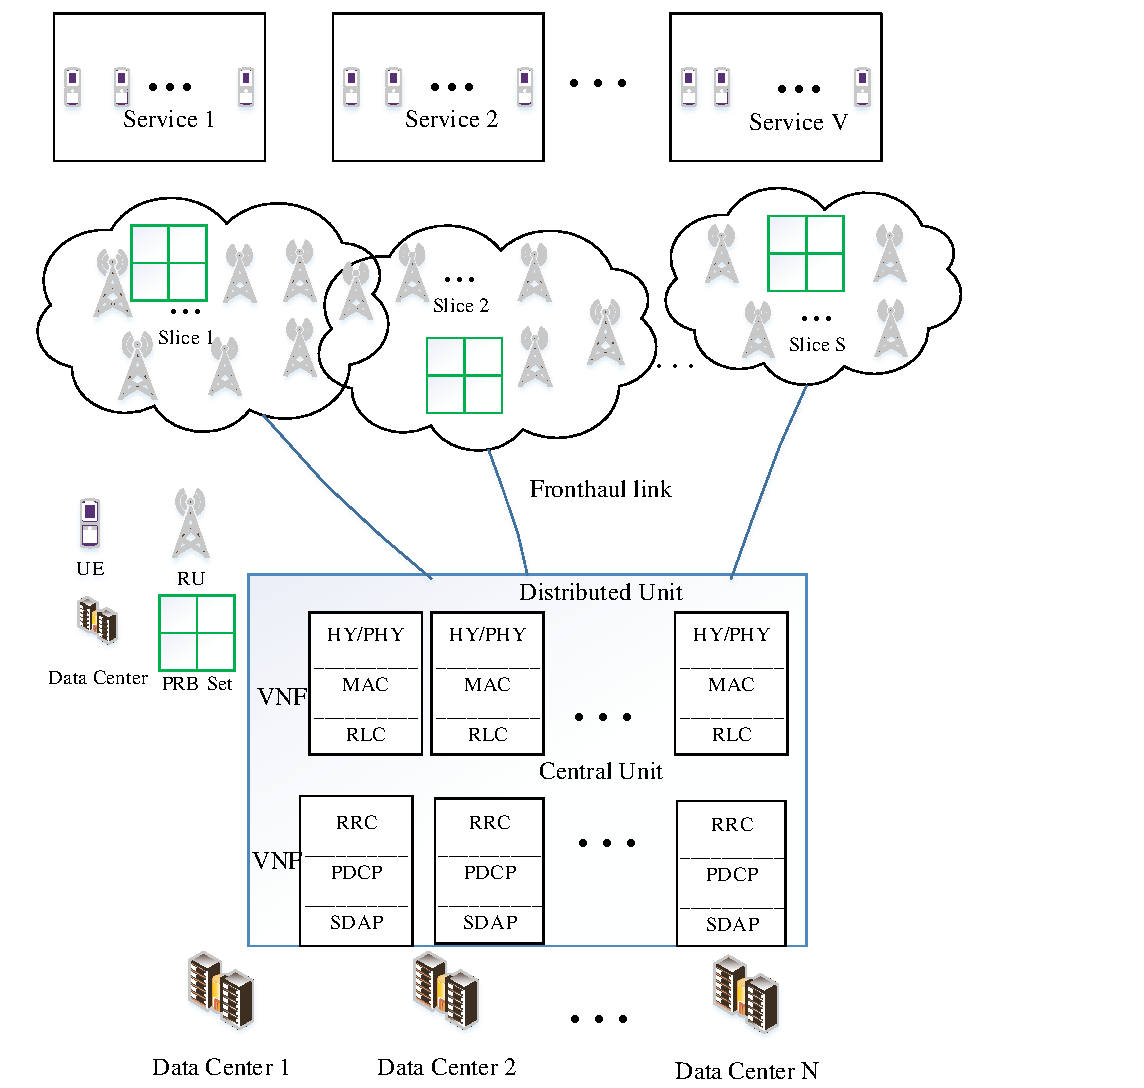
\includegraphics[scale=0.55]{./fig/c8.pdf}
	\caption{برش شبکه در ORAN}
	\label{fig:c11}
\end{figure}
در شکل \ref{fig:c11}
لینک فروسو در سیستم ORAN نشان داده شده است که بخش RAN به سه لایه تقسیم می‌گردد که شامل بخش RU، 
CU و
بخش DU می‌باشد.
بخش CUو DU برروی مرکز داده اجرا می‌شوند. کاربران براساس نیاز سرویسهای مختلف تقسیم شده‌اند.

نوآوری های این کار در ادامه بیان شده است.
\begin{itemize}
\item 
به طور همزمان برش شبکه و تخصیص منابع در سیستم
 ORAN
  در نظر گرفته شده است.
\item 
مسئله ی پذیرش کاربر و تخصیص خدمات به برش ها، و منابع فیزیکی بی سیم و مرکز داده به برش ها را به عنوان یک مسئله ی بهینه سازی حل می‌کنیم.
\item
از الگوریتمهای ابتکاری در جهت حل این مسائل برای رسیدن به پاسخ نسبتا بهینه استفاده کرده تا در کمترین زمان پاسخ نسبتا بهینه را بدهد.
\end{itemize} 
\section{مدل سیستم}
در این قسمت، سیستم مدل به صورت کامل مورد بررسی قرار می‌گیرد.
فرض می‌کنیم $S$ برش شبکه داریم که قرار است $V$ سرویس مختلف که شامل کاربرانی است که از سرویس خاص استفاده می‌نمایند را سرویس دهی نماید.
هر سرویس 
$v\in \{1,2,...,V \} $
شامل 
$U_v$
کاربر تک آنتنه می‌باشند که سرویس خاصی را درخواست می‌نماید.
هر برش شبکه 
$s \in \{1,2,...,S \}$
شامل 
$R_s$
واحد رادیویی،
$K_s$
بلوک های منابع فیزیکی، یک واحد توزیع شده و یک واحد مرکزی که شامل \lr{VNF} هایی می‌باشند.
همچنین برش های شبکه می‌توانند منابع مشترک داشته باشند.
تمام \lr{RU}هایی که به یک سرویس خاص خدمت رسانی می‌کنند به صورت مشارکتی سیگنال به تمام کاربران در آن سرویس ارسال می‌نمایند. 
\cite{motalleb2017optimal,mimoCran}
هر واحد رادیویی
$r \in \{1,2,...,R \}$
به یک واحد توزیع شده از طریق لینک فیبر نوری با ظرفیت \lr{fronthaul} 
محدود متصل می‌باشد.
در سیستم \lr{Open RAN}
دو لایه ی پردازشی که اولی در \lr{CU} و دومی‌در \lr{DU} قرار گرفته است که پردازش ها با \lr{VNF} ها صورت می‌گیرد.
لایه پایین تر (\lr{DU}) شامل 
\lr{high-PHY}
،
\lr{MAC}
و 
\lr{RLC}
می‌باشد و 
لایه ی بالاتر 
(\lr{CU})
شامل 
\lr{RRC}
،
\lr{PDCP}
و 
\lr{SDAP}
است.
فرض بر این است که $M_1$
\lr{VNF}
در \lr{DU}
و 
$M_2$
\lr{VNF}
در \lr{CU} قرار دارد.
هر \lr{VNF} به یک برش یا بیشتر تعلق دارد.
در $s^{th}$ امین برش شبکه $M_{s,1}$ 
\lr{VNF}
در \lr{DU}
و 
$M_{s,2}$
\lr{VNF}
در لایه ی \lr{CU} می‌باشد.
\lr{VNF}
های موجود در لایه ی \lr{DU} و \lr{VU} به ترتیب دارای ظرفیت محاسباتی 
$\mu_1$ 
و
 $\mu_2$
می‌باشند.
\subsection{نرخ قابل دسترس}
نرخ قابل دسترس برای $i^{th}$ امین کاربر در $v^{th}$امین سرویس به صورت زیر نوشته می‌شود
\begin{equation}\label{eq1}
\mathcal{R}_{u(v,i)} = B \log_2({1+ \rho_{u(v,i)}}),
\end{equation}
  که $B$ پهنای باند سیستم و 
  $\rho_{u(v,i)}$
  نسبت سیگنال به نویز $i^{th}$
  $i^{th}$ 
  امین کاربر در
   $v^{th}$
   امین سرویس
  می‌باشد 
  که از رابطه ی زیر بدست می‌آید
 \begin{equation}\label{eq2}
\rho_{u(v,i)} =  \frac{p_{u(v,i)}\sum_{s=1}^{S}|\bold{h}_{R_s,u(v,i)}^H \bold{w}_{R_s,u(v,i)}|^2 a_{v,s}}{BN_0 + I_{u(v,i)}},
\end{equation}
که   $p_{u(v,i)}$
نشان دهنده ی توان ارسالی توسط \lr{RU} به 
$i^{th}$ 
  امین کاربر در
   $v^{th}$
   امین سرویس
   است و 
 $\bold{h}_{R_s,u(v,i)} \in \mathbb{C}^{{R}_s}$
 بردار کانال گین لینک وایرلس از \lr{RU} ها در 
$s^{th}$
امین برش شبکه می‌باشد.
 همچنین 
$\bold{w}_{R_s,u(v,i)} \in \mathbb{C}^{{R}_s}$
نشان دهنده ی بردار بیم فرمینگ ارسالی برای \lr{RU}ها در $s$ امین برش شبکه به کاربر $i$ ام در سرویس $v$ ام می‌باشد.
   به علاوه، $BN_0$
   نشان دهنده ی توان نویز اضافه شونده ی گوسی می‌باشد و $I_{u(v,i)}$
   توان سیگنال تداخلی است.
همچنین $a_{v,s} \in \{0,1\}$
متغیر باینری است که نشان دهنده ی این است که برش شبکه ی $s$ به سرویس $v$ خدمات رسانی می‌کند یا نه.
درصورتی که 
 $a_{v,s} =1$
 برش شبکه ی $s$ به سرویس $v$ خدمات رسانی می‌کند. در غیر این صورت خدمت رسانی نمی‌کند.
\newline
برای بدست آوردن \lr{SNR} در فرمول \eqref{eq2}، 
فرض می‌شود که 
 $\bold{y}_{U_v}\in \mathbb{C}^{U_v} $
 بردار سیگنال دریافتی از همه ی کاربران در سرویس $v$ می‌باشد 
\begin{equation}\label{eq3}
\textstyle \bold{y}_{U_v} = \sum_{s = 1}^{S}\sum_{k=1}^{K_s} \boldsymbol{H}^H_{\mathcal{R}_s,\mathcal{U}_v} \
\mathfrak{y}_{R_s}\zeta_{U_v,k,s} a_{v,s}+ \boldsymbol{z}_{\mathcal{U}_v},
\end{equation}
که $\mathfrak{y}_{R_s} = \boldsymbol{W}_{\mathcal{R}_s,\mathcal{U}_v}\boldsymbol{P}_{U_v}^{\frac{1}{2}}\boldsymbol{x}_{\mathcal{U}_v}+ \boldsymbol{q}_{\mathcal{R}_s}$
و 
$\boldsymbol{x}_{ \mathcal{U}_v} = [x_{ u_{(v,1)}},...,x_{ u_{(v,\mathcal{U}_v)}}]^T \in \mathbb{C}^{{R}_s } $
نشان دهنده ی بردار سمبل ارسالی کاربران سرویس $v$ می‌باشد.
$\boldsymbol{z}_{U_v}$
نویز گوشی جمع شونده است و
$\boldsymbol{z_{U_v}} \backsim \mathcal{N}(0,N_0\boldsymbol{I}_{{U}_v})$
.
همچنین
$N_0$
توان نویز می‌باشد.
علاوه بر این
$\boldsymbol{q}_{R_s} \in \mathbb{C}^{{R}_s }  $
نشان دهنده ی نویز کوانتیزاسیون می‌باشد که از فشرده سازی سیگنال  در واحد توزیع شده بدست آمده است.
$\boldsymbol{P}_{U_v} = \diag{(p_{u{(v,1)}}, ..., p_{u{(v,\mathcal{U}_v)}})}$.
همچنین در اینجا، 
$\zeta_{k,s}^{U_v} \delequal \{\zeta_{k,s}^{u(v,1)},\zeta_{k,s}^{u(v,2)},...,\zeta_{k,s}^{u(v,N_{U_v})}\}$
و 
$\zeta_{k,s}^{u(v,i)} \in \{0,1\}$
پارامتر باینری می‌باشد که نشان دهنده ی این است که $i$ امین کابر در $v$امین سرویس امکان ارسال سیگنال خود را از طریق 
\lr{PRB}
$k$
ام دارد یا نه، در ضمن این \lr{PRB} 
 متعلق به برش $s$ ام می‌باشد و یا نه.
 $\boldsymbol{H}_{\mathcal{R}_s,\mathcal{U}_v}=\left[\boldsymbol{h}_{\mathcal{R}_s,u_{(v,1)}},\ldots,\boldsymbol{h}_{\mathcal{R}_s,v_{(v,\mathcal{U}_v)}}\right]^T  \in \mathbb{C}^{{R}_s\times {U}_v }$
نشان دهنده ی ماتریس کانال بین دسته واحد رادیویی 
 $\mathcal{R}_s$
 به دسته 
 $\mathcal{U}_v$
 کاربران می‌باشد.
بردار کانال بین $s$امین برش و $i$امین کابر در $v$امین سرویس $\boldsymbol{h}_{\mathcal{R}_s,u_{(v,i)}}\in \mathbb{C}^{{R}_s}$ به صورت زیر نشان داده شده است 
\begin{equation}
\boldsymbol{h}_{\mathcal{R}_s,u_{(s,i)}} = \boldsymbol{\beta}^\frac{1}{2}_{\mathcal{R}_s,u_{(v,i)}} \boldsymbol{g}_{\mathcal{R}_s,u_{(v,i)}},
\end{equation} 
که در اینجا 
$\boldsymbol{g}_{\mathcal{R}_s,u_{(v,i)}} \backsim \mathcal{N}(0,N_0\boldsymbol{I}_{\mathcal{U}_v})$
نشان دهنده ی بردار کانال فیدینگ سریع و تخت می‌باشد و
 $\boldsymbol{\beta}_{\mathcal{R}_s,u_{(v,i)}}=\text{diag}(b_{r_{(s,1),u_{(v,i)}}},\ldots,b_{r_{(s,\mathcal{R}_s),u_{(v,i)}}})$
 نشان دهنده ی ماتریس فیدینگ مقیاس بزرگ می‌باشد.
در اینجا فرض بر این است که اطلاعات حالت کانال \lr{CSI}، به صورت کامل می‌باشد.\newline
 $\boldsymbol{W}_{\mathcal{R}_s,\mathcal{U}_v} = [\boldsymbol{w}_{\mathcal{R}_s,u(v,1)},...,\boldsymbol{w}_{\mathcal{R}_s,u(v,U_v)}] \in \mathbb{C}^{{R}_s\times U_v} $
 بردار بیم فرمینگ \lr{zero forcing}
  می‌باشد که برای مینیمم کردن تداخل می‌باشد و بدین صورت است
\begin{equation}
\textstyle \boldsymbol{W}_{\mathcal{R}_s,\mathcal{U}_v} = \boldsymbol{H}_{\mathcal{R}_s,\mathcal{U}_v}(\boldsymbol{H}_{\mathcal{R}_s,\mathcal{U}_v}^H \boldsymbol{H}_{\mathcal{R}_s,\mathcal{U}_v})^{-1}.
\end{equation}  
توان تداخلی کابر $i$ام به سرویس $v$ام به صورت زیر بیان می‌شود
\begin{equation}
\begin{split}
 I_{u{(v,i)}} &=
 \underbrace{\sum_{s=1}^{S}\sum_{n=1}^{S}\sum_{\substack{l=1 \\ l\neq i}}^{{U}_v} \gamma_{1}  p_{u{(v,l)}}a_{v,s}\zeta_{n,s}^{u(v,i)}\zeta_{n,s}^{u(v,l)}}_{\text{\lr{(intra-service interference)}}}\\
&+ \underbrace{\sum_{\substack{y=1 \\ l\neq v}}^{V}\sum_{s=1}^{S}\sum_{n=1}^{S}\sum_{l=1}^{{U}_y} \gamma_{2}  p_{u{(y,l)}}a_{y,s} \zeta_{n,s}^{u(v,i)}\zeta_{n,s}^{u(y,l)}}_{\text{\lr{(inter-service interference)}}}\\
&+\underbrace{ \sum_{s=1}^{S} \sum_{j=1}^{{R}_s} {\sigma_q}_{r{(s,j)}}^2 |\boldsymbol{h}_{r{(s,j)}, u{(v,i)}}|^2 a_{v,s}}_{\text{\lr{(quantization noise interference)}}},
\end{split}
\end{equation}
که 
$\gamma_{1} =|\boldsymbol{h}_{\mathcal{R}_s, u{(v,i)}}^H \boldsymbol{w}_{\mathcal{R}_{s},u{(v,l)}}|^2$
و 
$\gamma_{2} =|\boldsymbol{h}_{\mathcal{R}_s, u{(v,i)}}^H \boldsymbol{w}_{\mathcal{R}_{s},u{(y,l)}}|^2$.
همچنین 

${\sigma_q}_{r_{(s,j)}}$
واریانس نویز کوانتیزاسیون
$j$
امین 
واحد رادیویی در برش $s$ می‌باشد.
سیگنال تداخلی برای هر کاربر از سیگنالهای کاربرانی بدست می‌آید که از \lr{PRB} مشترکی استفاده نموده اند.
درصورت قرار دادن $P_{max}$
به جای 
$p_{u{(v,l)}}$
و 
$p_{u{(y,l)}}$
باند بالایی  
$\bar{I}_{u{(v,i)}}$
برای 
$I_{u{(v,i)}}$
بدست می‌آید
بنابراین،
$\bar{\mathcal{R}}_{u{(v,i)}} \forall v , \forall i$ 
از قرار گرفتن 
$\bar{I}_{u{(v,i)}}$
به جای 
$I_{u{(v,i)}}$
در رابطه ی 
\eqref{eq1} و \eqref{eq2}
بدست می‌آید.
\newline
فرض کنید $\bar{p}_{r_{(s,j)}}$
نشان دهنده‌ی توان سیگنال ارسالی از $j$ امین واحد رادیویی در $s$ امین برش می‌باشد.
از رابطه ی \eqref{eq3} داریم
\begin{equation}
\bar{p}_{r{(s,j)}} = \sum_{v=1}^{V}\boldsymbol{w}_{r{(s,j)},\mathcal{U}_{v}} \boldsymbol{P}_{\mathcal{U}_v}^{\frac{1}{2}} \boldsymbol{P}_{\mathcal{U}_v}^{H \frac{1}{2}}   \boldsymbol{w}_{r{(s,j)},\mathcal{U}_{v}}^H a_{v,s} + \sigma_{q_{r(s,j)}}^2.
\end{equation}
در این صورت نرخ کاربران در لینک \lr{fronthaul} بین $j$امین واحد رادیویی در برش $s$ام با واحد توزیع شده ی موجود در این برش، بدین صورت می‌باشد  \cite{simeone2016cloud, 1111}
\begin{equation}
C_{R{(s,j)}} = \log{(1+\sum_{v=1}^{V}\frac{w_{r{(s,j)},\mathcal{D}_{s}} \boldsymbol{P}_{\mathcal{U}_v}^{\frac{1}{2}} \boldsymbol{P}_{\mathcal{U}_v}^{H \frac{1}{2}}   w_{r{(s,j)},\mathcal{U}_{v}}^H a_{v,s}}{ \sigma_{q_{r(s,j)}}^2})},
\end{equation}
که در اینجا 
$a_{v,s}$
متغیر باینری است که نشان دهنده ی این است که برش $s$ام به سرویس $v$ خدمات رسانی می‌کند یا نه.
\subsection{میانگین تاخیر}
فرض کنید ورود بسته های کاربران، فرآیند پوآسون با نرخ ورود 
$\lambda_{u(v,i)}$
برای $i$امین کاربر در سرویس $v$ ام می‌باشد.
بنابراین، در لایه ی واحد مرکزی (\lr{CU})، میانگین نرخ ورود داده ی کاربری که از خدمات برش $s$ استفاده می‌نماید 
$\alpha_{s_1} = \sum_{v=1}^{V}\sum_{u=2}^{U_v}a_{v,s}\lambda_{u(v,i)}$
می‌باشد. 
همچنین، میانگین نرخ داده ی ورودی در لایه ی \lr{DU}، تقریبا مساوی میانگین نرخ داده ی ورودی لایه ی اول 
$\alpha_{s} =\alpha_{s_1} \approx \alpha_{s_2}$
می‌باشد.
میانگین نرخ داده ی ورودی در لایه ی \lr{DU}، تقریبا برابر میانگین نرخ داده ی ورودی در لایه ی \lr{CU} می‌باشد $\alpha_{s} =\alpha_{s_1} \approx \alpha_{s_2}$.
در اینجا فرض بر این است کهدر هر لایه متعادل کننده ی ترافیک موجود است که ترافیک ورودی را به طور مساوی بین \lr{VNF} ها تقسیم می‌نماید\cite{frdl,luong2018novel,luong2018novel1}.
فرض کنید پردازش باند پایه هر \lr{VNF}، بوسیله ی پردازش صف \lr{M/M/1} نشان داده می‌شود.
هر بسته بوسیله ی یکی از \lr{VNF}های برش شبکه، پردازش می‌شود.
بنابراین، میانگین تاخیر برش $s$ در لایه ی اول و دوم با استفاده از مدل \lr{M/M/1} به این صورت نشان داده می‌شود
\begin{equation}
\begin{split}
d_{s_1} &= \frac{1}{\mu_1 - \alpha_{s}/{M_{s,1}}},\\
d_{s_2} &= \frac{1}{\mu_2 - \alpha_{s}/{M_{s,2}}}.
\end{split}
\end{equation}
در اینجا
$1/\mu_1$ و $1/\mu_2$
میانگین زمان سرویس دهی در لایه ی اول و دوم به ترتیب می‌باشند.
$\alpha_{s}$
نرخ ورودی است که توسط متعادل کننده ی ترافیک به طور مساوی بین \lr{VNF} ها تقسیم می‌شود.
نرخ ورودی هر \lr{VNF} در هر لایه از برش \lr{s}، $\alpha_{s}/{M_{s,i}}$ $ i \in \{1,2\}$ می‌باشد.
$d_{s_{tr}}$
تاخیر ارسال برای برش $s$ در لینک وایرلس می‌باشد.
نرخ داده ی ورودی لینک وایرلس برابر نرخ داده ی ورودی متعادل کننده ی ترافیک برای هر برش است
\cite{frdl}.
همچنین زمان سرویس برای صف ارسال در هر برش $s$ دارای توزیع نمایی با میانگین $1/(R_{{tot}_s})$
است و می‌توان به صورت صف \lr{M/M/1} مدل کرد  
\cite{frdl,luong2018novel,luong2018novel1,guo2016exploiting}.
بنابراین میانگین تاخیر لایه ی ارسال بدین صورت است
\begin{equation}
 d_{s_{tr}} = \frac{1}{R_{{tot}_s} - \alpha_{s}};
\end{equation}
 $R_{{tot}_s} =  \sum_{v=1}^{V}\sum_{u=2}^{U_v}a_{v,s}R_{u(v,i)}$ 
 کل نرخ قابل دسترس در هر برش می‌باشد که به سرویس خاص، تخصیص داده است.
میانگین تاخیر در هر برش نیز بدین صورت است
\begin{equation}
D_{s} = d_{s_1} + d_{s_2} + d_{s_{tr}} \forall s.
\end{equation}
\subsection{مرکز داده ی فیزیکی}
هر \lr{VNF}
نیازمند منابع فیزیکی است که شامل حافظه، نگهدارنده و پردازشگر می‌باشد.
فرض کنید منابع مورد نیاز برای $f$ امین \lr{VNF} در برش $s$ ام به صورت زیر می‌باشد
 \begin{equation}
\bar{\Omega}_{s}^f = \{\Omega_{M,{s}}^f, \Omega_{S,{s}}^f, \Omega_{C,{s}}^f \},
\end{equation}
که در اینجا 
 $\bar{\Omega}_{s}^f\in \mathbb{C}^{3}$
 و
$\Omega_{M,{s}}^f, \Omega_{S,{s}}^f, \Omega_{C,{s}}^f$
به ترتیب نشان دهنده ی مقدار حافظه، نگهدارنده و پردازشگر می‌باشد.
همچنین مقدار کل حافظه، نگهدارنده و پردازشگر برای همه \lr{VNF} ها در یک برش به این صورت تعریف می‌شود
\begin{equation}
\textstyle \bar{\Omega}_{\mathfrak{z},s}^{tot} = \sum_{f=1}^{M_{s_1} + M_{s_2}}\bar{\Omega}_{\mathfrak{z},s}^f \;\; \mathfrak{z} \in \{M, S, C\}.
\end{equation}
همچنین $D_c$ مرکز داده برای سرویس دهی به \lr{VNF} ها می‌باشد. هر مرکز داده شامل تعدادی سرور برای سرویس دهی است.
مقدار حافظه، نگهدارنده و پردازشگر به ترتیب با 
$\tau_{M_{j}}, \tau_{S_{j}}$
و
$\tau_{C_{j}} $
برای 
$j^{th}$
امین مرکز داده به ترتیب زیر می‌باشد.
\begin{equation*}
\tau_j = \{\tau_{M_{j}}, \tau_{S_{j}}, \tau_{C_{j}} \},
\end{equation*}
در این مدل سیستم، 
تخصیص منابع فیزیکی به \lr{VNF} ها در نظر گرفته شده است. 
در اینجا فرض بر این است که $y_{s,d}$ متغیر صفر و یکی است که در صورت یک بودن نشان می‌دهد مرکز داده ی $d$ام به $s$امین برش، منابع فیزیکی اختصاص داده است.
\subsection{صورت مساله}
یک معیار مهم برای سنجش بهینگی یک سیستم ، بهره وری انرژی است که نسبت نرخ کل به توان کل می‌باشد.
\begin{equation}
\textstyle \eta(\boldsymbol{P},\boldsymbol{A}) := \frac{\sum\limits_{v=1}^{V} \sum\limits_{k=1}^{{U}_v}\mathcal{R}_{u_{(v,k)}} }{\sum\limits_{s=1}^{S} \sum\limits_{i=1}^{{R}_s}\bar{p}_{r_{(s,i)}}} = \frac{\mathfrak{R}_{tot}(\boldsymbol{P},\boldsymbol{A})}{P_r^{{tot}}(\boldsymbol{P},\boldsymbol{A})},
\end{equation}
که در اینجا، 
 $P_r^{tot}(\boldsymbol{P},\boldsymbol{A}) = \sum\limits_{s=1}^{S}\sum\limits_{i=1}^{{R}_s}\bar{p}_{r_{(s,i)}}$
 توان کل مصرفی تمام واحد های رادیویی در یک برش می‌باشد.
همچنین 
 $\mathfrak{R}_{tot}(\boldsymbol{P},\boldsymbol{A}) = \sum\limits_{v=1}^{V} \sum\limits_{k=1}^{{U}_v}\mathcal{R}_{u_{(v,k)}} $
 نرخ تمام کاربران مصرفی تمام سرویس ها می‌باشد.
فرض کنید توان مصرفی پردازش باند پایه در هر مرکز داده ی $d$ که به \lr{VNF} های یک برش $s$ متصل می‌باشد با   
$\phi_{s,d}$
نشان داده شده است.
بنابراین می‌توان توان کل سیستم را برای کلیه مرکز داده های فعال که به برش شبکه سرویس دهی می‌کنند، بدین صورت نشان داد
\begin{equation*}
\textstyle \phi_{tot} = \sum_{s=1}^{S}\sum_{d=1}^{D_c}y_{s,d}\phi_{s,d}.
\end{equation*}
همچنین ، یک تابع هزینه برای سرویس دهی\lr{VNF} ها توسط مرکز داده ها بدین عنوان تعریف شده است
\begin{equation}\label{eqpsi}
\textstyle  \psi_{tot} = \phi_{tot} - \nu \sum_{s=1}^{S}\sum_{d=1}^{D_c}\sum_{v=1}^{V}y_{s,d}a_{v,s}
\end{equation}
که $\nu$
متغیر طراحی برای ارزش بین اولین ترم 
\eqref{eqpsi}
 است که عبارت است از کل مصرف انرژی منابع فیزیکی و ترم دوم که مقدار برش های پذیرفته شده برای داشتن منابع فیزیکی نشان داده شده است.
هدف ما این است که مجموع نرخ را به حداکثر رسانده و توان حاصل از کل (حداکثر توان تمام واحد های رادیویی و کل مصرف انرژی پردازش باند پایه را در کلیه مرکز داده ها) به طور همزمان و با وجود محدودیت هایی که به شرح زیر نوشته شده است ، به حداکثر برساند.
\begin{subequations}
\begin{alignat}{4}
\max\limits_{\boldsymbol{P}, \boldsymbol{A}, \boldsymbol{Y} }   \quad &  \eta(\boldsymbol{P},\boldsymbol{A})+ \varphi \frac{1}{\psi_{tot}(\boldsymbol{Y})} \\
\text{subject to} \quad  & \bar{p}_{r_{(s,i)}} \leq P_{max} \quad \forall s, \forall i,
 \label{c11} \\
&p_{u_{(v,k)}}  \geq 0  \quad \forall v, \forall k,\label{c12} \\
&\mathcal{R}_{u_{(v,k)}} \geq  \mathcal{R}_{u_{(v,k)}}^{min} \quad \forall v, \forall k,\label{c13} \\
&C_{r_{(s,i)}} \leq C_{r_{(s,i)}}^{max} \quad \forall s, \forall i, \label{c14}\\
&D_{s} \leq D_{s}^{max} \quad \forall s,\label{c15} \\
& \textstyle  \sum_{s=1}^{S}a_{v,s} \geq 1 \quad \forall s, \label{c21} \\
& \textstyle  \sum_{d=1}^{D_c}\sum_{v=1}^{V}y_{s,d}a_{v,s} \geq 1\times\sum_{v=1}^{V}a_{v,s} \forall s,\label{c23} \\
 &\textstyle \sum_{s=1}^{S} y_{s,d} \bar{\Omega}_{\mathfrak{z},s}^{tot}  \leq   \tau_{\mathfrak{z}_d}  \forall d, \forall \mathfrak{z}\in \mathcal{E}; \label{c22}
\end{alignat}
\label{constraints}
\end{subequations}
در اینجا،
$\boldsymbol{P} =[p_{u(v,k)}] \:\: \forall v , \forall k $
ماتریس توان برای کاربران است،
$\boldsymbol{A} =[a_{v,s}] \:\: \forall v , \forall s $
نشان دهنده ی
متغیر باینری برای اتصال برشها به سرویسها و
$\boldsymbol{Y} =[y_{s,d}]  \:\: \forall s ,  \forall d $
متغیر باینری برای اتصال
مرکز داده ی فیزیکی به VNFها می‌باشد.
همچنین
$\varphi$ 
متغیر وزنی برای ارزش گزاری بین ترم اول و دوم تابع هدف است.
\eqref{c11}
و
\eqref{c12}
به ترتیب
نشان دهنده ی این است که توان واحد رادیویی از حدی بیشتر نشده و توان هر کاربر یک عدد صحیح مثبت است.
علاوه براین
\eqref{c13}
منجر به افزایش نرخ هرکاربر از حد مورد نیاز می‌باشد.
 \eqref{c14}
  و 
  \eqref{c15}
  به ترتیب
  محدودیت ظرفیت لینک
  fronthaul 
  و محدودیت مورد نیاز برای تاخیر سیگنال ارسالی
  را نشان می‌دهد.
  \eqref{c21}
 تضمین می‌کند که هر سرویس
 به حداقل یک
 برش شبکه متصل شده است.
همچنین،
\eqref{c23}
تضمین می‌کند که هر برش که شامل VNF هایی در دو لایه است،
به حداقل یک مرکز داده متصل می‌شود.
در \eqref{c22} 
$\mathcal{E} = \{M,S,C\}$ 
و شرطها ضمانت می‌کند که منابع فیزیکی کافی برای VNFها وجود دارد.\newline
مسئله‌ی بهینه‌سازی \eqref{constraints}
قابل جداسازی به دو مسئله‌ی بهینه‌سازی کوچکتر می‌باشد زیرا متغیرها می‌تواند به صورت مجزا بدست آیند. ابتدا نیاز به حل مسئله‌ی اول 
داریم و پس از حل آن
$\boldsymbol{P}$
و
$\boldsymbol{A}$
بدست می‌آید. سپس با حل مسئله‌ی دوم و قرار دادن مقدار بهینه‌ی  $ \boldsymbol{A}$ در مسئله
خروجی  $ \boldsymbol{Y}$
بدست می‌آید.
مسئله‌ی اول به صورت زیر می‌باشد.
\begin{subequations}
	\begin{alignat}{4}
		\max\limits_{\boldsymbol{P}, \boldsymbol{A} }   \quad &   \eta(\boldsymbol{P},\boldsymbol{A})\\
		\text{\lr{subject to}} \quad  & \bar{p}_{r_{(s,i)}} \leq P_{max} && \quad \forall s, \forall i,   \\
		&p_{u_{(v,k)}}  \geq 0  &&\quad \forall v, \forall k, \\
		&\mathcal{R}_{u_{(v,k)}} \geq  \mathcal{R}_{u_{(v,k)}}^{min} && \quad \forall v, \forall k, \\
		&C_{r_{(s,i)}} \leq C_{r_{(s,i)}}^{max}  &&\quad \forall s, \forall i,\label{cc14} \\
		&D_{s} \leq D_{s}^{max}  &&\quad \forall s, \label{cc15} \\
		& \textstyle  \sum_{s=1}^{S}a_{v,s} \geq 1 &&\quad \forall s.
	\end{alignat}
	\label{constraints1}
\end{subequations}
مسئله‌ی دوم نیز بدین صورت بیان می‌شود.
\begin{subequations}
	\begin{alignat}{4}
		\min\limits_{\boldsymbol{y} }   \quad &   \psi_{tot}(\boldsymbol{Y})\\
		\text{\lr{subject to}} \quad & \textstyle \sum_{d=1}^{D_c}\sum_{v=1}^{V}y_{s,d}a_{v,s} \geq 1\times\sum_{v=1}^{V}a_{v,s} \quad \forall s, \\
		&\textstyle  \sum_{s=1}^{S} y_{s,d} \bar{\Omega}_{\mathfrak{z},s}^{tot}  \leq   \tau_{\mathfrak{z}_d}  \quad \forall d, \forall \mathfrak{z}\in \mathcal{E};  \label{eqomega}
	\end{alignat}
	\label{constraints23}
\end{subequations}
\section{روش ابتکاری استفاده شده}\label{proposedmethod}
در این بخش از روش ابتکاری برای حل مسئله \eqref{constraints1}
استفاده می‌کنیم که یک مسئله‌ی غیر‌محدب همراه با محاسبات طولانی است.
برای حل مسئله همانطور که قبلا بیان شد، مسئله به دو بخش مختلف و مجزا تجزیه می‌شود که به صورت تکراری حل می‌گردد.
در بخش اول در ابتدای کار در اولین حلقه با قرار دادن $\boldsymbol{P} = P_{max}$ و $\eta = 0$ در رابطه‌ی \eqref{constraints1}
مقدار $\boldsymbol{A}$ بدست می‌آید.  سپس  با  $\boldsymbol{A}$ بدست آمده، $\boldsymbol{P}$ را در معادله‌ی \eqref{constraints1} بروزرسانی می‌کنیم. این معادله قابل تبدیل به یک مسئله‌ی محدب است و با روشهای محدب حل می‌شود. بعد از حل این مسئله، 
$\boldsymbol{P}$و $\eta$
بروزرسانی شده و این چرخه‌ی دو بخشی تا همگرا شدن ادامه دارد.
\subsection{بخش اول مسئله‌ی اول}\label{firstsub}
الگوریتم تکرار شده برای بدست آوردن $\boldsymbol{A}$ در اینجا اجرا می‌گردد. بخش اول مسئله‌ی اول از جنس بسته‌بندی جعبه به صورت سه بعدی می‌باشد که یک مسئله‌ی NP-Hard است و برای حل آن نیاز به الگوریتمهای ابتکاری داریم.
در 
\cite{3dbin}،
الگوریتم ابتکاری براساس مرتب‌سازی جعبه‌ها براساس اندازه‌گیری بیان شده‌است.
در این الگوریتم، ابتدا سرویسها بر اساس  مقدار نیازمندی کاربران به صورت نزولی قرار گرفته‌اند. همچنین برشهای شبکه نیز براساس جمع وزن‌داری از ظرفیت منابع فیزیکی و پردازشی خود به صورت نزولی قرار گرفته‌اند. سپس در صورت اعمال شرط 
\eqref{c11}،
 \eqref{c12}،
 \eqref{c13}
 و 
\eqref{c14} 
برش شبکه به سرویس تخصیص داده می‌شود و در غیر این صورت به برش شبکه‌ی بعدی برای اعمال شرط‌ها انتقال داده می‌شود.
جزئیات الگوریتم موردنظر در \ref{alg}
و براساس الگوریتم
 \cite{3dbin}
 و روش
  BFD\LTRfootnote{Best Fit Decreasing}
  بیان شده است.

	\begin{algorithm}
		\caption{اتصال سرویس به برش شبکه}\label{alg}
		\begin{latin}
		\begin{algorithmic}[1]
			
			\State{Sort services according to the number of UEs, priority and their requirements in the descending order.}
			\State{Sort slices according to the weighted linear combination of number of PRBs, RUs and VNFs and the capacity of their resources in the descending order.}
			\For {$i \gets 1$ to $S$}
			\For {$j \gets 1$ to $V$}
			\State{Set $a_{i,j} = 1$}
			\State{Obtain Parameters of Systems (power, delay, rate and capacity of fronhaul links)}
			\If {conditions \eqref{c11}, \eqref{c12}, \eqref{c13} and \eqref{c14} are not applied}
			\State{Set $a_{i,j} = 0$;}
			\Else
			\State{break from inner loop;}
			\EndIf
			\State{\textbf{end if}}
			\EndFor
			\State{\textbf{end for}}
			\EndFor
			\State{\textbf{end for}}
		\end{algorithmic}
	\end{latin}
	\end{algorithm}

\subsection{بخش دوم مسئله‌ی اول}\label{secondsub}
در این بخش با فرض ثابت قرار دادن  $\boldsymbol{A}$
توان کاربران در هر سرویس بدست می‌آید.
\begin{theorem}\label{t2}
	بهره‌وری انرژی زمانی بدست می‌آید که
	\begin{equation}\label{q2}
		%\begin{split}
		\max \limits_{\boldsymbol{P}} (\mathfrak{R}_{tot}(\boldsymbol{P}) - \eta^* P_{r_{tot}}(\boldsymbol{P}))=
		\mathfrak{R}_{tot}(\boldsymbol{P}^*) - \eta^* P_{r_{tot}}(\boldsymbol{P}^*) =0.
		%\end{split}
	\end{equation}
\end{theorem}
\begin{proof}
	مراجعه به  \cite[\lr{Appendix A}]{aaa}
\end{proof}
در بخش دوم مسئله‌ی اول از الگوریتم تکراری و تابع لاگرانژ برای حل استفاده شده است. 
از آنجایی که تداخل تابعی از توان کاربران است، برای سادگی فرض باند بالای $\bar{I}_{u_{(v,i)}}$ برای آن می‌کنیم. برای اینکه بتوانیم 
\eqref{constraints1}
را به صورت فرم استاندارد بهینه سازی محدب درآوریم، نیازمند این هستیم که متغیرهای روابط
\eqref{cc14} 
و
\eqref{cc15}
 را   ($p_{r_{(s,i)}} = \sigma_{q_{r(s,j)}}^2\times 2^{C_{r_{(s,i)}}}$ و $1/(D_{s}- d_{s_1} + d_{s_2})+\alpha_s$ تغییر دهیم.
فرض کنید $\boldsymbol{\lambda}$ ، $\boldsymbol{\mu}$، $\boldsymbol{\xi}$ و $\boldsymbol{ \kappa}$  ماتریسهای ضرایب لاگرانژ می‌باشد که دارای مقادیر مثبت غیر‌صفرند. تابع لاگرانژ بدین صورت نوشته می‌شود.

\begin{subequations}\label{lagrang}
	\begin{alignat}{4}
		\mathcal{L}(\boldsymbol{P}; \boldsymbol{\lambda}, \boldsymbol{\chi}, \boldsymbol{\mu}, \boldsymbol{ \xi}, \boldsymbol{ \kappa}) & = \sum\limits_{v=1}^{V} \sum\limits_{k=1}^{U_v}\mathcal{\bar{R}}_{u_{(v,k)}}
		- \eta \sum\limits_{v=1}^{V} \sum\limits_{i=1}^{\mathcal{R}_s}\bar{p}_{r_{(s,i)}}\\
		&+\sum\limits_{v=1}^{V} \sum\limits_{k=1}^{U_v} \lambda_{u_{(v,k)}} (\mathcal{\bar{R}}_{u_{(v,k)}}-\mathcal{R}_{u_{(v,k)}}^{max})\\
		&- \sum\limits_{s=1}^{S} \sum\limits_{i=1}^{R_s} \mu_{r_{(s,i)}} (\bar{p}_{r_{(s,i)}}-P_{max})\\
		&- \sum\limits_{s=1}^{S} \sum\limits_{i=1}^{R_s} \xi_{r_{(s,i)}} (\bar{p}_{r_{(s,i)}}-\sigma_{q_{r(s,i)}}^2 2^{C_{r_{(s,i)}}^{max}}).\\
		&+ \sum\limits_{v=1}^{V} \sum\limits_{k=1}^{U_v} \kappa_{u_{(v,k)}} \sum\limits_{s=1}^{S}(R_{u_{(v,k)}} -\mathfrak{D_s})a_{v,s}.
	\end{alignat}
\end{subequations}
که دراینجا $\mathfrak{D_s}=\frac{1}{D_{s}^{max}-d_{s_1}-d_{s_2}}+\alpha_s$.
توان بهینه از \eqref{lagrang}
بدین صورت خواهد بود

\begin{equation}
	p_{u(v,i)}^{*} = [\frac{\mathfrak{y}_{u(v,i)}\mathfrak{w}_{u(v,i)}-\mathfrak{x}_{u(v,i)}\mathfrak{z}_{u(v,i)}}{\mathfrak{x}_{u(v,i)}\mathfrak{w}_{u(v,i)} }]^+
\end{equation}
که دراینجا 
 $\mathfrak{y}_{u(v,i)}= (\lambda_{u(v,i)}+\kappa_{u_{(v,k)}}+1)\frac{B}{Ln_2}$
 و
$\mathfrak{w}_{u(v,i)} = \sum_{s=1}^{S}|\bold{h}_{R_s,u(v,i)}^H \bold{w}_{R_s,u(v,i)}|^2 a_{v,s}$. 
همچنین
$\mathfrak{z}_{u(v,i)} = BN_0 + \bar{I}_{u(v,i)}$ و $\mathfrak{x}_{u(v,i)} = \sum\limits_{s=1}^{S} \sum\limits_{i=1}^{R_s} ( \mu_{r_{u(s,i)}} + \xi_{r_{(s,i)}}+\eta)||w_{r_{(s,j)},u_{(v,i)}}||^2$.
با استفاده از روش sub-gradient توان بهینه $\boldsymbol{P}$ بدست می‌آید\cite{mimoCran}.
\subsection{حل دو بخش مسئله‌ی اول به صورت تکراری}
در \eqref{firstsub} و \eqref{secondsub}
جزئیات حل هر بخش از مسئله‌ی اول آورده شده است.
در ابتدا با ثابت نگه‌داشتن $\boldsymbol{P} = P_{max}$
و $\eta = 0$
مقدار $\boldsymbol{A}$
در مسئله‌ی \eqref{constraints1}
و با استفاده از الگوریتم \eqref{alg}
بدست می‌آید. 
پس از آن در بخش دوم، با استفاده از روش 
sub-gradient
مقدار
 $\boldsymbol{P}$ 
بدست می‌آید. 
بعد از بدست آوردن $\boldsymbol{P}$
مقدار $\eta$
نیز دوباره به‌روز رسانی می‌شود.
 سپس الگویتم با مقادیر جدید توان و بهره‌وری انرژی دوباره تکرار می‌گردد تا همگرا شود.
در اینجا الگوریتم حل مسئله‌ی اول به صورت الگوریتم \eqref{alg2} است.

\begin{algorithm}
	\caption{برش شبکه و تخصیص منابع}\label{alg2}
	\begin{latin}
	\begin{algorithmic}[1]
		\State{Set the maximum number of iterations $I_{max}$, convergence condition $\epsilon_{\eta}$  and the initial value $\eta^{(1)} = 0$}
		\State{Set $\boldsymbol{P} = \boldsymbol{P}_{max}$}
		\For{$counter \gets 1$ to $I_{max}$}
		\State{Achieve $\boldsymbol{A}$ by applying Algorithm \eqref{alg}}
		\State{Obtain $\boldsymbol{P}$ by using sub-gradient method which is mentioned in \eqref{secondsub}.}
		\If{$ \mathfrak{R}_{tot}(\boldsymbol{P}^{(i)},\boldsymbol{A}^{(i)}) - \eta^{(i)} P_{r_{tot}}(\boldsymbol{P}^{(i)},\boldsymbol{A}^{(i)}) < \epsilon_{\eta} $}
		\State{Set $\boldsymbol{P}^*= \boldsymbol{P}^{(i)} $, $\boldsymbol{A}^*= \boldsymbol{A}^{(i)} $   and  $ \eta^{*} =\eta^{(i)} $;}
		\State{break;}
		\Else
		\State{$i= i+1$, Setting $\boldsymbol{P} = \boldsymbol{P}^{(i)}$ ;}
		\EndIf
		\State{\textbf{end if}}
		\EndFor
		\State{\textbf{end for}}
	\end{algorithmic}
	\end{latin}
\end{algorithm}
\subsection{ حل مسئله‌ی دوم}
در این بخش می‌خواهیم مسئله‌ی \eqref{constraints23} را حل نماییم که قرارگیری منابع مجازی در منابع فیزیکی می‌باشد به‌طوری که تابع هزینه‌ی  $\psi_{tot}$ کمینه شود. این مسئله از جنس مسئله‌ی سه بعدی بسته‌بندی جعبه است که NP-Hard می‌باشد. 
برای بدست‌آوردن مقدار بهینه‌ی $\boldsymbol{Y}$ الگوریتم ابتکاری برای حل مسئله‌ی سه بعدی بسته‌بندی جعبه ارائه شده است.
جزئیات الگوریتم در \eqref{alg3} نوشته شده است. در این الگوریتم، در ابتدا برشهای شبکه و مرکز داده ها را بر اساس  جمع وزنی آنها به صورت نزولی مرتب می‌کنیم (خط \ref{31} و \ref{32} الگوریتم \ref{alg3}).
در اینجا، پارامتر وزندار برای $\Omega_{\mathfrak{z},s}^{tot}$ و $\tau_j^\mathfrak{z}$ بدین صورت تعریف می‌کنیم.
\begin{equation}\label{wt}
	\begin{split}
		\hat{\Omega}_{s}^{tot} &= w_M \bar{\Omega}_{M,s}^{tot} + w_S \bar{\Omega}_{S,s}^{tot} + w_C \bar{\Omega}_{C,s}^{tot} \\
		\hat{\tau}_j &= w_M \tau_{{j}}^M + w_S \tau_{{j}}^S + w_C \tau_{{j}}^C,
	\end{split}
\end{equation}
که دراینجا، $\boldsymbol{w} = \{w_M, w_S, w_C\}$ وزن حافظه، نگهداری و CPU می‌باشد
که  از الگوریتم مورد استفاده برای بسته‌بندی سه بعدی در مقاله‌ی 
\cite{3dbin}
استفاده شده است.
در مرحله دوم، ما تخصیص را از بیشترین برش های مورد نیاز به DC با بیشترین منابع فیزیکی شروع می‌کنیم(از خط \ref{33} تا \ref{34} الگوریتم \ref{alg3}).
 بعد از تخصیص برش شبکه به مرکز داده، در صورتی که یکی از برشهای شبکه توسط مرکز داده پذیرش نشود، برای بخش بعدی جاگذاری می‌رود
 (از خط \ref{35} تا \ref{36} الگوریتم \ref{alg3}).
 در آخر، اگر مرکز داده‌ای با میزان منابع کمتر آزاد باشد و بتواند برشهای یک مرکز داده‌ی دیگر با میزان منابع بیشتر را سرویس‌دهی کند، 
 تخصیص منابع بین این دو مرکز داده جابه‌جا می‌شود(خط \ref{37} از الگوریتم \ref{alg3}). 
\begin{algorithm}
	\caption{قرار گیری منابع مجازی در منابع فیزیکی}\label{alg3}
	\begin{latin}
	\begin{algorithmic}[1]
		\State Sort Slices according to $\hat{\Omega}_{s}^{tot} , \forall s$ in descending order.\label{31}
		\State Sort DCs according to $\hat{\tau}_j , \forall j$ in descending order. \label{32}
		\State $\boldsymbol{Y} = \boldsymbol{0}$
		\For {$d \gets 1$ to $D_c$}\label{33}
		\For {$s \gets 1$ to $S$}
		\If {$\sum_{d=1}^{D_c}y_{s,d}==0$ and $\bar{\Omega}_{\mathfrak{z}(s)}^{tot} \leq \tau_{\mathfrak{z}_j} \forall \mathfrak{z}, \forall s$  }
		\State Set $y_{s,d} = 1$;
		\State {$\tau_j^{\mathfrak{z}}$ $\gets$ {$\tau_j^{\mathfrak{z}} - \bar{\Omega}_{\mathfrak{z},s}^{tot}$}} $\mathfrak{z}\in \{M,S,C\}$
		\EndIf
		\State \textbf{end if}
		\EndFor
		\State \textbf{end for}
		\EndFor
		\State \textbf{end for} \label{34}
		\State  $ind_{rem} = \{s|({\sum_{d=1}^{D_c}y_{s,d}==0})\}$ \label{35}
		\State Sort remaining amount of DCs same as before in descending order.
		\State Sort remaining slices same as before in descending order.
		\For {$r \gets 1$ to $S_{rem}$}
		\For {$n \gets 1$ to $D_c$}
		\State Set $y_{s,d} = 1$;
		\State {$\bar{\Omega}_{{\mathfrak{z}},s}^{tot}$ $\gets$ {$\bar{\Omega}_{{\mathfrak{z}},s}^{tot}- \tau_j^{\mathfrak{z}}$}}
		\If {$\bar{\Omega}_{s}^{tot}==0$}
		\State Set $y_{s,d} = 1$;
		\State {$\tau_j^{\mathfrak{z}}$ $\gets$ {$\tau_j^{\mathfrak{z}} - \bar{\Omega}_{\mathfrak{z},s}^{tot}$}} $\mathfrak{z}\in \{M,S,C\}$
		\State {break inner loop}
		\EndIf
		\State \textbf{end if}
		\EndFor
		\State \textbf{end for}
		\EndFor
		\State \textbf{end for} \label{36}
		\State Remapping DCs must be done to prevent wasting Energy \label{37}
	\end{algorithmic}
\end{latin}
\end{algorithm}
\section{نتایج عددی}\label{simul}
در این بخش نتایج عددی برای مسئله ی اصلی بیان می‌شود.
ابتدا برای مسئله‌ی اول نمودارهای شبیه‌سازی را رسم می‌کنیم.
\begin{table}
	\caption {پارامترهای شبیه‌سازی} \label{table:1a}
	\begin{latin}
	\begin{center}
		\begin{tabular}{||c c ||}
			\hline
			Parameter & Value \\ [0.5ex]
			\hline\hline
			Noise power & -174dBm\\
			\hline
			Bandwidth & 120 KHZ \\
			\hline
			Maximum transmit Power of each RU & 40dBm \\
			\hline
			Minimum delay &  300usec \\
			\hline
			Maximum fronthaul capacity  & 200 bits/sec/Hz \\
			\hline
			Minimum data rate &  10 bits/sec/Hz \\ [1ex]
			\hline
		\end{tabular}
	\end{center}
	\end{latin}
\end{table}
در شکل \ref{fig:f1a}، بهره‌وری انرژی برای دو سری تعداد سرویس مختلف با تعداد کاربر متفاوت در هر سرویس بدست‌آمده‌است.
پارامترهای شبیه‌سازی در جدول \ref{table:1a} قرار داده‌شده‌است. تعداد منابع فیزیکی ۱۰ تا می‌باشد.
روش بهینه برای بدست آوردن $\boldsymbol{A}$ توسط MOSEK بدست آمده و برای بدست آوردن $\boldsymbol{P}$ از CVX در متلب استفاده شده است و به صورت متناوب این دو ماتریس به‌روزرسانی می‌شوند. 
روش بهینه،  
$0.1bits/J/Hz$ 
از روش آورده شده بهتر است (برای  $V = 6$ و $E[U_v] = 10$).
همچنین 
$0.09bits/J/Hz$
از روش آورده شده بهتر است (برای  $V = 3$ و $E[U_v] = 10$).
همانطور که در شکل مشخص است بهره‌وری انرژی با افزایش تعداد کاربران افزایش می‌یابد.
\begin{figure}%[H]
	\centering
	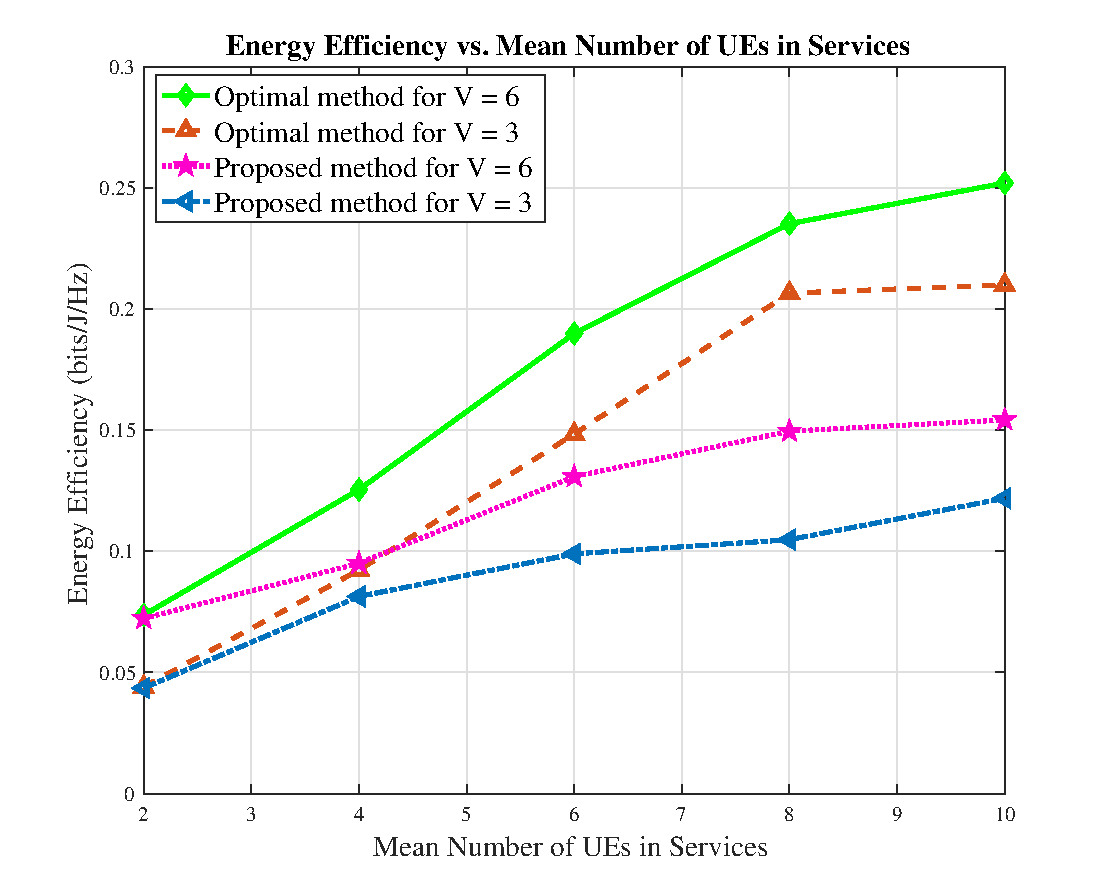
\includegraphics[width=\linewidth]{./fig/fig1_last}
	\caption{بهره‌وری انرژی براساس تعداد کاربران در هر سرویس}
	\label{fig:f1a}
\end{figure}
در شکل \ref{fig:f1a2}
بهره‌وری انرژی براساس تعداد بلوکهای منابع فیزیکی برای ۶ سرویس با تعداد کاربر به طور میانگین ۳ تا رسم شده است. همانطور که در نمودارها مشخص است با افزایش تعداد PRB، تداخل کاربران کم شده و بهره‌وری انرژی افزایش می‌یابد و الگوریتم پیشنهادی به روش بهینه نزدیک می‌گردد.  
\begin{figure}%[H]
	\centering
	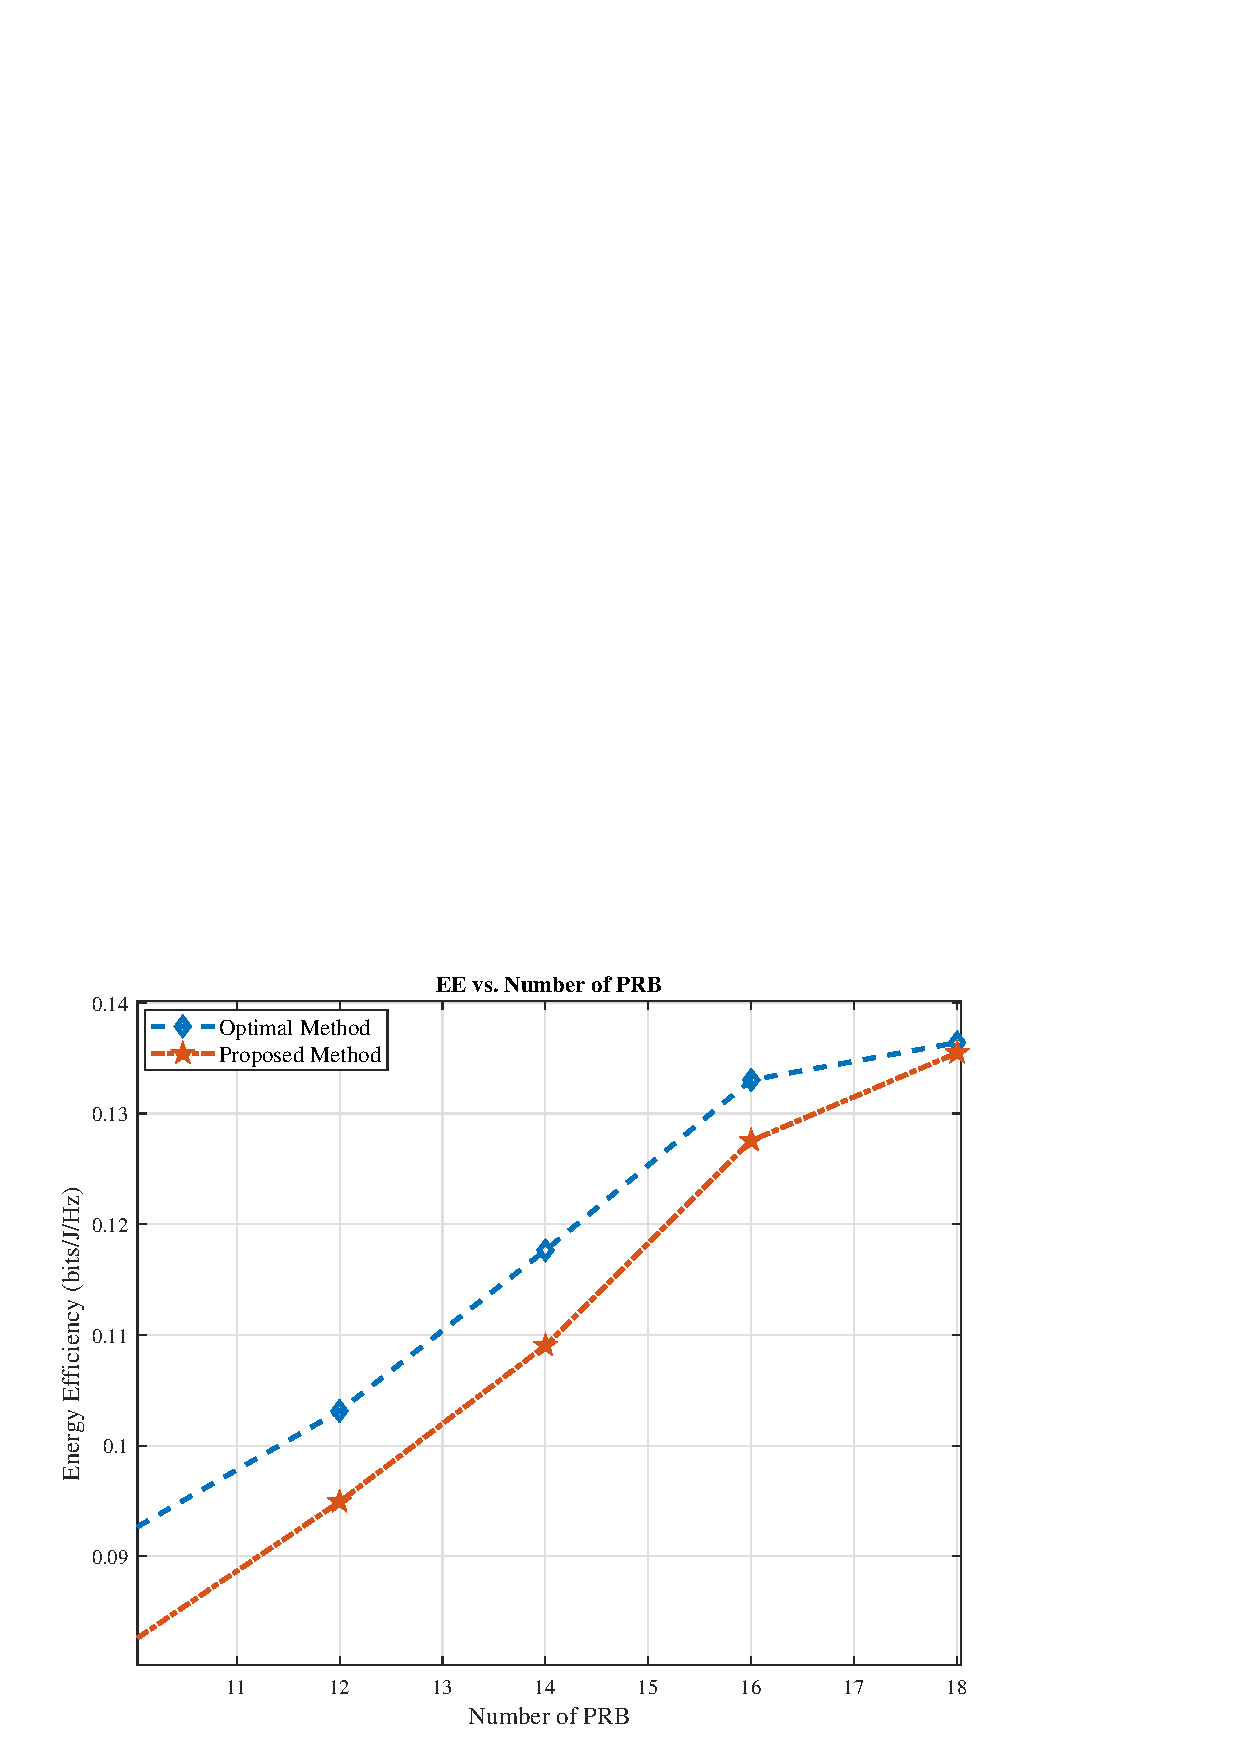
\includegraphics[width=\linewidth]{./fig/fig_prb1}
	\caption{بهره‌وری انرژی براساس تعداد بلوکهای منابع فیزیکی}
	\label{fig:f1a2}
\end{figure}

در شکل \ref{fig:f1a3}
بهره‌وری انرژی براساس تعداد سرویسای مختلف با فرض وجود ۲ کاربر در هر سرویس به طور میانگین، رسم شده است. همانطور که در نمودارها مشخص است با افزایش تعداد سرویسها، بهره‌وری انرژی که مجموع نرخهای کاربران برروی توان آن است، افزایش می‌یابد و الگوریتم پیشنهادی به روش بهینه به نسبت نزدیک است‌.  
\begin{figure}%[H]
	\centering
	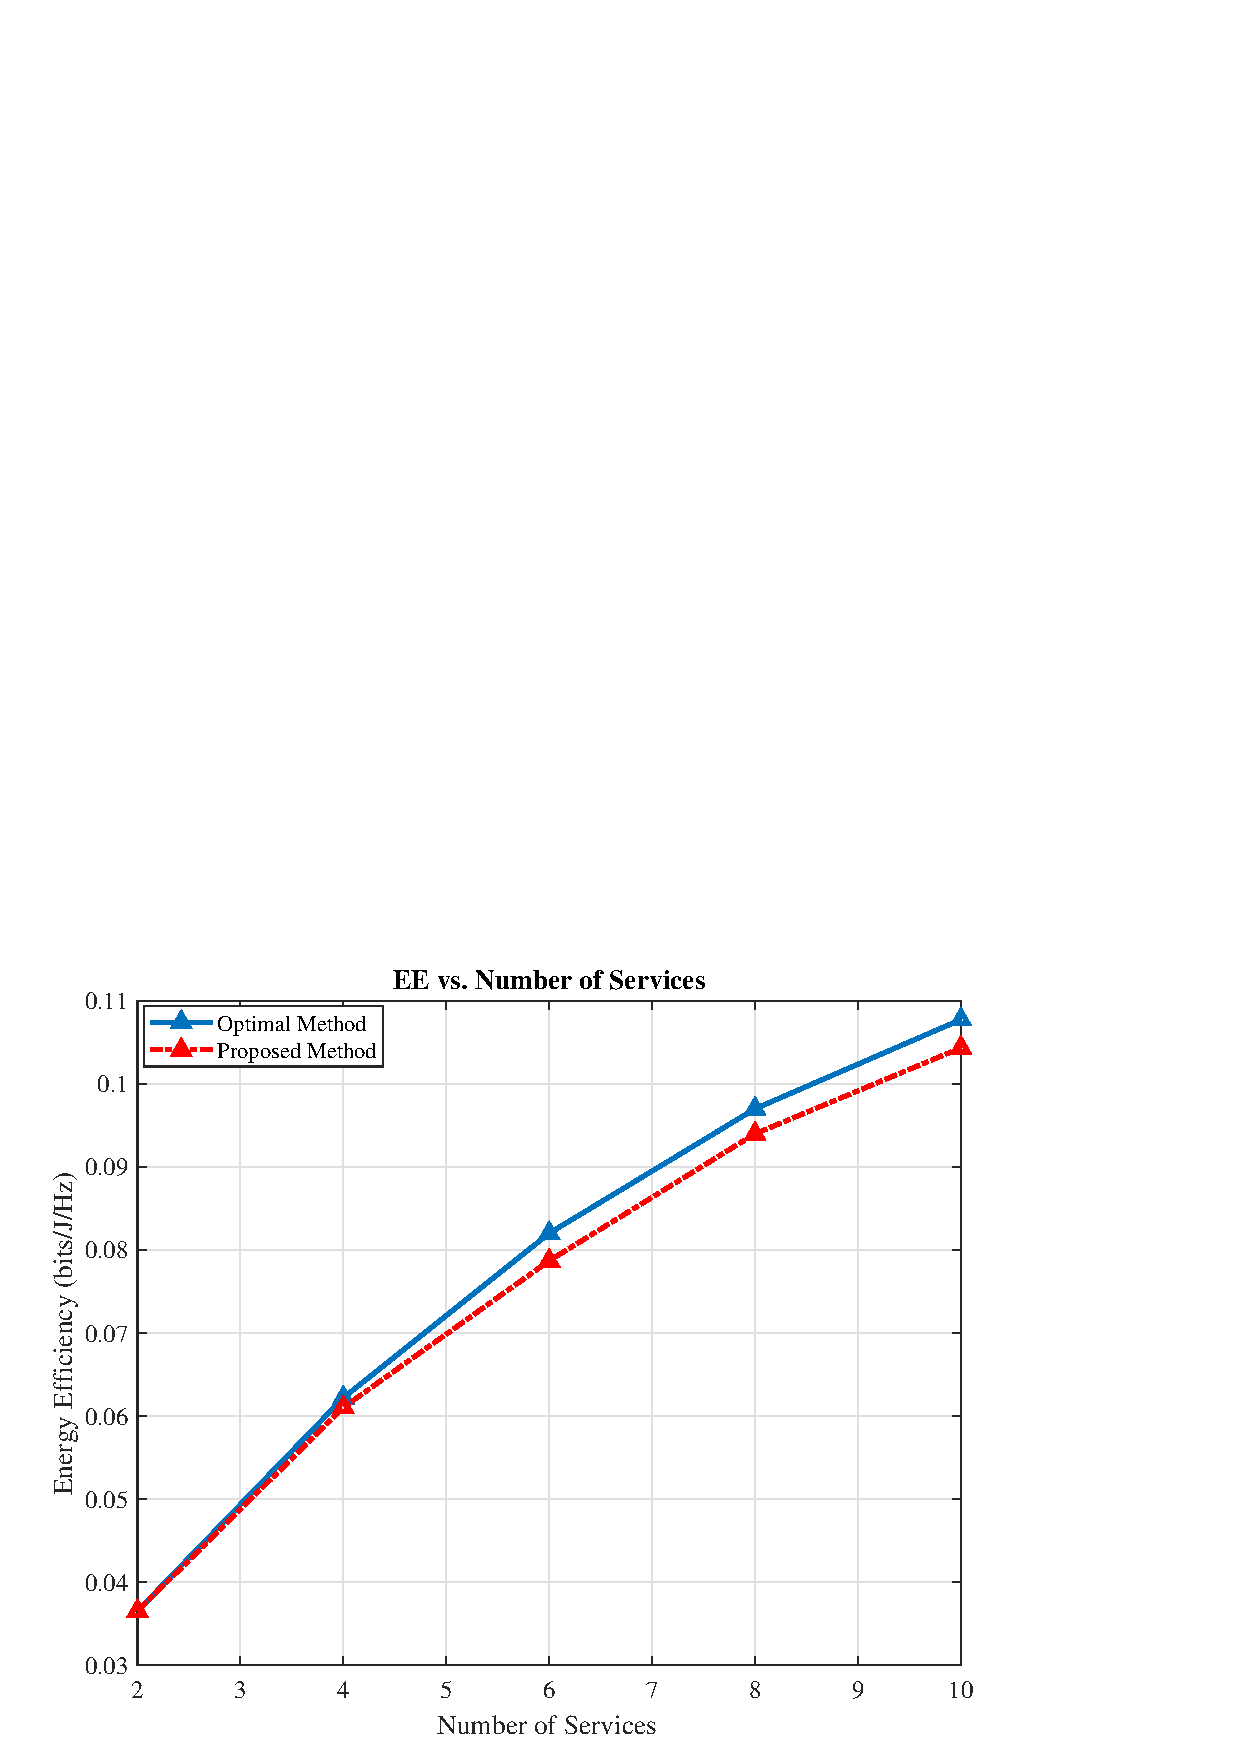
\includegraphics[width=\linewidth]{./fig/fig_service1}
	\caption{بهره‌وری انرژی براساس تعداد سرویسهای مختلف }
	\label{fig:f1a3}
\end{figure}


حال به نتایج عددی مسئله‌ی دوم می‌پردازیم.
در شکل \ref{fig:f1}، نسبت برشهای پذیرفته شده برای دو تعداد مختلف مرکز داده با تعداد برشهای مختلف رسم شده است. پارامترهای شبیه‌سازی در جدول \ref{table:1} آورده شده است. همچنین داریم 
 $w_C = 320$،
 $w_S = 100$و 
 $w_M =1$.
 در این شبیه‌سازی ترم دوم رابطه‌ی \eqref{eqpsi}، مورد اهمیت قرار گرفته شده است و پارامتر طراحی $\nu$ مقدار بالایی دارد.
 همچنین فرض شده که تنها یک مرکز داده می‌تواند هر برش را سرویس دهد. روش ارائه شده در الگوریتم  \ref{alg3} آورده شده و روش بهینه با استفاده از MOSEK بدست می‌آید.
 وقتی دو مرکز داده یا DC داریم، روش پیشنهادی و روش بهینه تقریباً همان نسبت برش های پذیرفته شده را دارند. اما با افزایش تعداد DC ها به پنج ، عملکرد روش پیشنهادی کاهش می‌یابد.
 با استفاده از پنج DC ، تفاوت بین روش پیشنهادی و روش بهینه در بدترین حالت (44 برش) حدود 23 درصد است.

\begin{small}
	\begin{table}
		\caption {پارامترهای شبیه‌سازی} \label{table:1}
		\begin{latin}	
		\begin{center}
			\begin{tabular}{||c c ||}
				\hline
				Parameter & Value \\ [0.5ex]
				\hline\hline
				Mean of CPU for DCs & 320GHz\\
				\hline
				Mean of Memory for DCs & 1T\\
				\hline
				Mean of Storage for DCs & 100T \\
				\hline
				Mean of CPU for Slices & 32GHz\\
				\hline
				Mean of Memory for Slices & 100G\\
				\hline
				Mean of Storage for Slices & 10T \\ [1ex]
				\hline
			\end{tabular}
		\end{center}
	\end{latin}
	\end{table}
\end{small}
\begin{figure}%[H]
	\centering
	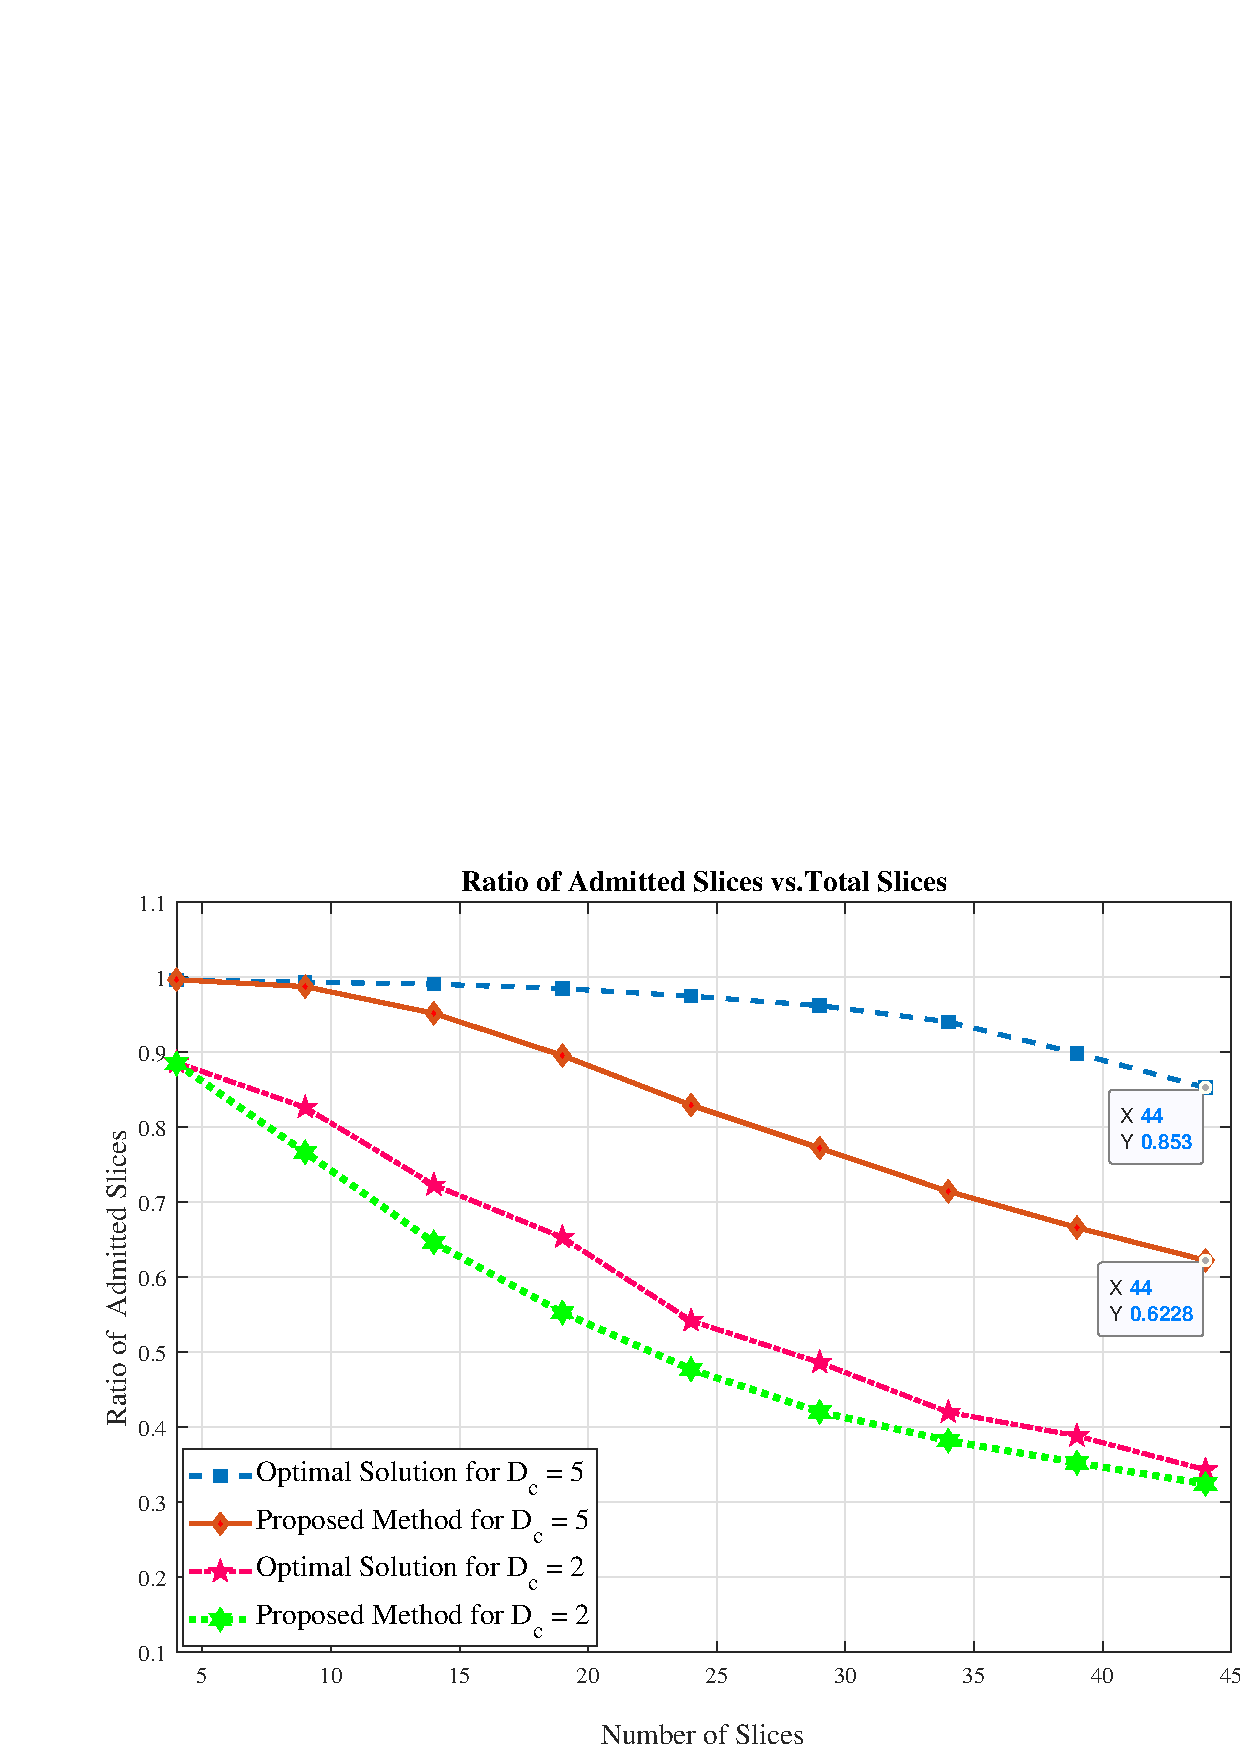
\includegraphics[scale = 0.5]{./fig/f112}
	\caption{نسبت برش های پذیرفته شده فقط به یک 	DC در مقابل برش های کل}
	\label{fig:f1}
\end{figure}
در شکل \ref{fig:f2}
نرمالیزه‌ی مصرف منابع بر‌اساس تعداد برشهای شبکه آورده شده است. پارامترهای شبیه‌سازی در جدول \ref{table:1}، قرار داده شده و 
($w_C = 320$, $w_S = 100$, $w_M =1$).
در این شبیه سازی ، فرض کنید تعداد DC ها کاملاً کافی باشد تا تمام برش ها را پوشش دهد و پارامتر طراحی شده $ \ nu $ کم فرض شود ، بنابراین ما روی اولین ترم \eqref{eqpsi} تمرکز کردیم.
با این حال ، اگر هر قطعه باقی مانده باشد ، می‌تواند توسط بیش از یک DC سرویس دهی شود.
بهینه بودن محل قرارگیری برشها در منابع DC بر اساس مصرف توان DC ها اندازه گیری می‌شود.
در اینجا مقدار منابع  مصرف DC نشده نشان داده شده است. برای ۱۰ برش شبکه اختلاف بین مقدار بهینه و روش اعمال شده ۱۵ درصد می‌باشد. 
\begin{figure}%[H]
	\centering
	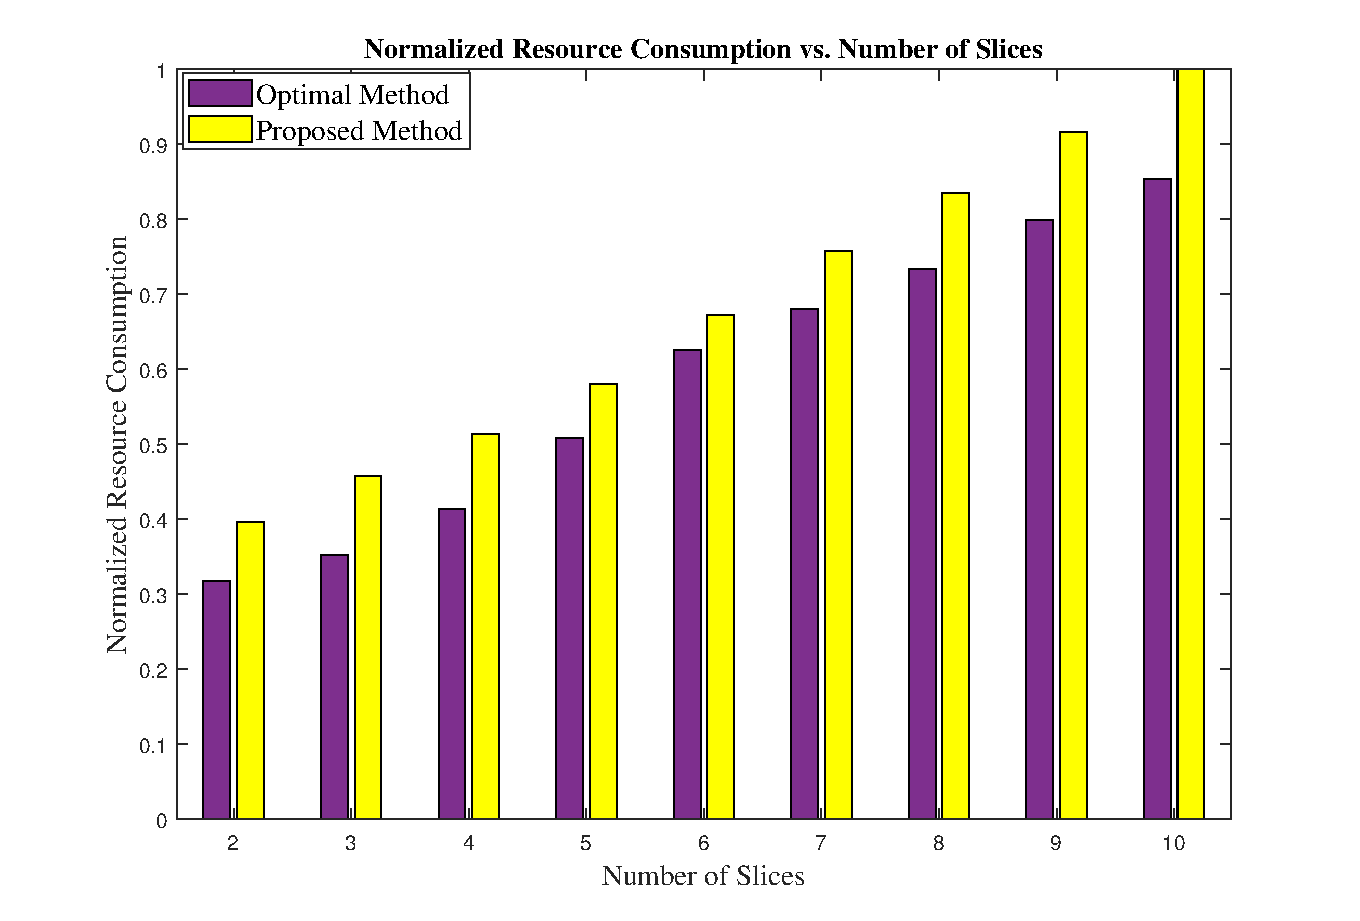
\includegraphics[scale = 0.5]{./fig/fig22_last} %[width=\linewidth] 
	\caption{نرمالیزه‌ی مصرف منابع بر‌اساس تعداد برشها}
	\label{fig:f2}
\end{figure}
\section{نتیجه‌گیری}
در این فصل، همزمانی برش شبکه و تخصیص توان در سیستم ORAN آمده‌است. فرض بر این است که کاربران بر اساس نیازهایشان به سرویسهای مختلف طبقه بندی می‌شوند. همچنین ، تعدادی برش نیز در خدمت این سرویسها قرار می‌گیرد. هر برش شبکه شامل تعدادی PRB، RU، و VNFهایی است که اعمال CU و DU را انجام می‌دهد. ظرفیت محدود لینک fronthaul برای اتصالات فیبر بین RU و DU در نظر گرفته شده است.
هدف به حداکثر رساندن مجموع نرخ و به حداقل رساندن مصرف توان و هزینه انرژی مراکز داده به طور همزمان است.
این مسئله به دو زیر مسئله تجزیه می‌شود. هر زیر مسئله به طور جداگانه توسط یک الگوریتم ابتکاری حل می‌شود. با استفاده از نتایج عددی، روش اکتشافی را تأیید کرده و عملکرد الگوریتم ها را مطالعه می‌کنیم.
برای مسئله‌ی اول بازدهی انرژی در مقابل تعداد UE در هر سرویس به تصویر کشیده شده است.
با افزایش میانگین تعداد کاربران در هر سرویس، از بازدهی انرژی بیشتر می‌شود.
برای مسئله دو، دو شکل نشان داده شده است.
در شکل اول، نسبت برش های پذیرفته شده که فقط به یک DC متصل می‌شوند، برای تعداد برش های مختلف مشخص شده است.
در شکل دوم، مصرف منابع نرمال DC ها به تصویر کشیده شده است.
در هر شکل، الگوریتم ابتکاری با روش بهینه مقایسه شده و تفاوت بین آنها بحث شده است.

		% فصل سوم: روش تحقیق
\chapter{تخصیص برش شبکه به صورت دینامیکی}
\section{مقدمه}
در این فصل هدف تخصیص برش شبکه به صورت می‌باشد. در فصل قبلی مدل سیستم به طور کامل نوشته شده است و در حالت آفلاین حل گردیده است، در این فصل پارامترها مورد نیاز را نسبت به فصل قبلی کمتر کرده و با استفاده از روش دینامیکی در هر لحظه از زمان به حل سیستم می‌پردازیم. برای حل این سیستم از روش یادگیری تقویتی عمیق استفاده می‌کنیم.
در بخش اول صورت مسئله‌ی بخش رادیویی نوشته می‌شود. سپس به صورت مسئله و مدل سیستم بخش هسته می‌پردازیم و در نهایت روش حل هر دو مسئله و نتایج عددی آن بیان می‌شود.
\section{ مدل سیستم و صورت مسئله‌ی اول}
در این بخش هدف برش شبکه در بخش رادیویی سیستم می‌باشد. دراینجا، مسئله‌ی اول فصل قبلی ساده شده و به روش دینامیکی حل می‌شود.   
همانند سیستم فصل قبل، فرض می کنیم $S$ برش شبکه داریم که قرار است $V$ سرویس مختلف که شامل کاربرانی است که از سرویس خاص استفاده می‌نمایند را سرویس دهی نماید.
هر سرویس 
$v\in \{1,2,...,V \} $
شامل تعدادی کاربر تک آنتنه می باشند که سرویس خاصی را درخواست می‌نماید.
هر برش شبکه
$s\in \{1,2,...,S \} $
 شامل تعدادی
 PRB
  RU،
   BBU، 
   و
    VNF 
 می‌باشد.
در این بخش سعی برا‌ین است که در ابتدا مسئله را به ساده‌ترین حالت ممکن حل نماییم. فرض می‌کنیم سه مدل سرویس مختلف داریم که سرویسهای دسته‌ی اول نیازمند تاخیر خاص و سرویسهای دسته‌ی دوم نیازمند داشتن تاخیر کم هستند و سرویس سوم نیازمند داشتن هر دو حالت تاخیر کم و نرخ زیاد است.
در بخش اول این مسئله، هدف بیشینه‌سازی تعدای سرویسهای پذیرفته شده می‌باشد. در اینجا فرض براین است که تعداد برشهاس شبکه محدود می‌باشد. فرض می‌کنیم هر سرویس $v$ دارای اولویت $p_v$ می‌باشد. 
همچنین فرض براین است که هر سرویس شامل ماکسیمم $U_v$ کاربر است و به طور میانگین کاربران آن نیازمند داشتن نرخ بیشتر از $R_v$ و تاخیر کمتر از $D_v$ هستند. درصورتی که کاربری از دسته‌ی اول باشد 
$D_v =  M$ 
که $M$ برای تاخیر یک عدد بزرگ می‌باشد.
و در صورتی که سرویس از دسته‌ی دوم باشد 
$R_v = N $
که $N$ یک عدد کوچک برای نرخ می‌باشد.
صورت مسئله به صورت \eqref{eqmain} می‌باشد.
در اینجا برای سادگی فرض براین است که هر سرویس به ماکسیمم یک برش شبکه متصل می‌گردد. در اینجا هدف حل مسئله در هر اسلات زمانی t می‌باشد.
 هدف در اینجا بیشینه سازی تعداد سرویسهای پذیرفته شده توسط برشهای شبکه می‌باشد به صورتی که شرط تاخیر و نرخ سرویس را ضمانت کنند.
\begin{subequations}
	\begin{alignat}{4}
		\max\limits_{\boldsymbol{a}(t) }   \quad &   \sum_{s=1}^{S(t)}\sum_{v=1}^{V(t)} p_v a_{v,s}(t)\\
		\text{\lr{subject to}} \quad & \textstyle \sum_{s=1}^{S(t)} D_s(t) a_{v,s} \leq D_v(t)  \forall v, \\
		&\textstyle   \sum_{s=1}^{S(t)} R_s(t) a_{v,s}(t) \geq R_v(t)  \forall v \label{eqmain}
	\end{alignat}
	\label{constraints2}
\end{subequations}
 برای اینکه معادله‌ی 
 \eqref{eqmain}
 را به فرم مسئله‌ی کوله‌پشتی دربیاوریم، از آنجایی که فرض کردیم هر سرویس به ماکسیمم یک برش شبکه متصل می‌شود، می‌توان معادله بدین صورت نوشت:
 \begin{subequations}
 	\begin{alignat}{4}
		\max\limits_{\boldsymbol{a}(t) }   \quad &   \sum_{s=1}^{S(t)}\sum_{v=1}^{V(t)} p_v a_{v,s}(t)\\
		\text{\lr{subject to}} \quad & \textstyle \sum_{s=1}^{S(t)} D_s(t) a_{v,s} \leq D_v(t)  \forall v, \\
 		&\textstyle   \sum_{s=1}^{S(t)} \frac{1}{R_s(t)} a_{v,s}(t) \leq \frac{1}{R_v(t)}  \forall v \label{eqmain1}
 	\end{alignat}
 	\label{constraints2}
 \end{subequations}
که در اینجا، معادله‌ی \eqref{eqmain1}
یک معادله‌ی کوله‌پشتی دو بعدی می‌باشد.
برای حل این مسئله، از روش یادگیری تقویتی استفاده می‌شود.
\section{ مدل سیستم و صورت مسئله‌ی دوم}
در این بخش سعی شده، مسئله‌ی دوم فصل قبل به صورت ساده شده با روش دینامیکی حل شود. عنوان این مسئله، جاگزاری VNFها برروی مراکز داده می‌باشد.
فرض براین است که $S$ برش شبکه داریم که هر برش شبکه s
$s\in \{1,2,...,S \} $
می‌باشد. هر برش شبکه شامل تعدادی VNF است که
هر \lr{VNF}
نیازمند منابع فیزیکی است که شامل حافظه، نگهدارنده و پردازشگر می باشد.
فرض کنید برای سادگی مسئله برای هر VNF به مقدار کافی حافظه و نگهددارنده در مراکز داده داریم و تنها منبع مورد نیاز برای $f$ امین \lr{VNF} در برش $s$ ام مقدار پردازنده است که به صورت $\bar{\Omega}_{s}^f$ می باشد 
%\begin{equation}
%	\bar{\Omega}_{s}^f = \{\Omega_{M,{s}}^f, \Omega_{S,{s}}^f, \Omega_{C,{s}}^f \},
%\end{equation}
که در اینجا 
$\bar{\Omega}_{s}^f\in \mathbb{C}^{1}$
و
%$\Omega_{M,{s}}^f, \Omega_{S,{s}}^f, \Omega_{C,{s}}^f$
%به ترتیب نشان دهنده ی مقدار حافظه، نگهدارنده و پردازشگر می باشد.
%همچنین مقدار کل حافظه، نگهدارنده و پردازشگر برای همه \lr{VNF} ها در یک برش به این صورت تعریف می شود
\begin{equation}
	\textstyle \bar{\Omega}_{s}^{tot} = \sum_{f=1}^{M_{s}}\bar{\Omega}_{s}^f %\;\; \mathfrak{z} \in \{M, S, C\}.
\end{equation}
همچنین $D_c$ مرکز داده برای سرویس دهی به \lr{VNF} ها می باشد. هر مرکز داده شامل تعدادی سرور برای سرویس دهی است.$M_s$ تعداد کل VNFها در sامین برش شبکه است.
مقدار پردازشگر 
%$\tau_{M_{j}}, \tau_{S_{j}}$
%و
$\tau_{j} $
برای 
$j$
امین مرکز داده  می‌باشد.
%\begin{equation*}
%	\tau_j = \{\tau_{M_{j}}, \tau_{S_{j}}, \tau_{C_{j}} \},
%\end{equation*}
در این مدل سیستم، 
تخصیص منابع فیزیکی به \lr{VNF} ها در نظر گرفته شده است. 
در اینجا فرض بر این است که $y_{s,d}$ متغیر صفر و یکی است که نشان میدهد مرکز داده ی $d$ ام به $s$ امین برش متصل است یا نه. 
همانند فصل قبل، 
فرض کنید توان مصرفی پردازش باند پایه در هر مرکز داده ی $d$ که به \lr{VNF} های یک برش $s$ متصل می باشد در هر زمان t با   
$\phi_{s,d}(t)$
نشان داده شده است.
بنابراین می توان توان کل سیستم را برای کلیه مرکز داده های فعال که به برش متصل هستند ،بدین صورت نشان داد
\begin{equation*}
	\textstyle \phi_{tot}(t) = \sum_{s=1}^{S}\sum_{d=1}^{D_c}y_{s,d}\phi_{s,d}(t).
\end{equation*}
همچنین ، یک تابع هزینه برای قرار
همچنین فرض کنید در هر زمان قرار دادن هر مجموعه‌ی جدید VNFهای برش شبکه s برروی مرکز داده d مقدار انرژی اضافی را بدین صورت به سیستم اعمال کنند.
\begin{equation*}
	\textstyle \phi_{diff}(t) = \sum_{s=1}^{S}\sum_{d=1}^{D_c}[y_{s,d}(t)-y_{s,d}(t-1)]^+\phi_{s,d}^{new}(t).
\end{equation*}
%%
تابع هزینه‌ی قرارگیری VNFها برروی DCها بدین صورت است
\begin{equation}\label{eqpsi}
	\textstyle  \psi_{tot}(t) = \phi_{tot}(t) + \phi_{diff}(t)
\end{equation}
در اینجا هدف کمینه کردن مقدار انرژی کل در هر زمان، با فرض اینکه مجموع VNFهای برشهای تخصیص یافته به هر مرکز داده مقدار کافی پردازنده داشته باشند. در اینجا فرض براین است که برشهای شبکه که قبلا به سرویسها اختصاص داده شده، می‌بایست در مرکز داده قرار داده شوند و تعداد مراکز داده به اندازه‌ی کافی زیاد هستند، هدف کمینه کردن انرژی است به صورتی که کمترین تعداد مرکز داده‌ها استفاده شوند.
\begin{subequations}
	\begin{alignat}{4}
		\min\limits_{\boldsymbol{y} }   \quad &   \psi_{tot}(\boldsymbol{Y})(t)\\
		\text{s. t.} \quad & \textstyle \sum_{d=1}^{D_c} y_{s,d}(t) \geq 1 \quad \forall s, \\
		&\textstyle  \sum_{s=1}^{S} y_{s,d}(t) \bar{\Omega}_{s}^{tot}  \leq   \tau_{d} \quad  \forall d, \forall ;  \label{eqomega}
	\end{alignat}
\end{subequations}
این مسئله به فرم مسئله‌ی بسته‌بندی جعبه قابل بیان است.
\section{حل مسئله به‌روش یادگیری تقویتی}
دراینجا از روش یادگیری تقویتی در حل دو مسئله‌ی بالا استفاده می‌نماییم.
در روش یادگیری تقویتی، یک عامل سعی می‌کند رفتار بهینه را در یک محیط مشخص پیدا کند. این پروسه‌ی تعاملی، به صورت پروسه‌ی تصمیم‌گیری مارکوف مدل می‌شود که شامل $(S,A,R,P,\gamma)$  می باشد.
S
نشان‌دهنده‌ی ماتریس فضای حالت و A بردار رفتار می‌باشد. R نیز پاداش عمل است. 
$P(.|s,a)$
احتمال انتقال و
 $\gamma \in (0,1]$
 فاکتور تخفیف می‌باشد.
 سیاست 
$\Pi(.|s)$
نگاشتی از حالت به توزیع اعمال می‌باشد.
تابع مقدار-حالت برای حالت s تحت سیاست $\Pi(.|s)$ را با  
$V^{\Pi}(s)$
نشان می‌دهند که مقدار بازده مورد انتظار در حالت s تحت سیاست $\Pi(.|s)$
می‌باشد. مقدار ارزش انجام عمل a در حالت s تحت سیاست $\Pi(.|s)$ 
را با
 $Q^{\Pi}(s,a)$
 نمایش می‌دهیم.
 که روابط زیر را براین اساس داریم.
 \begin{equation}
	V^{\Pi}(s) = \mathbb{E}_{\Pi,P}[\sum_{t=0}^{\infty}\gamma^tR_t|S_0=s]
 \end{equation}
و تابع ارزش عمل بدین صورت است

 \begin{equation}
	Q^{\Pi}(s,a) = \mathbb{E}_{\Pi,P}[\sum_{t=0}^{\infty}\gamma^tR_t|S_0=s,A_0=a]
\end{equation}
  که در اینجا 
  $\mathbb{E}$
  میانگین می‌گیرد.
  باتوجه به رابطه‌ی بلمن، داریم:
 \begin{equation}
	V^{\Pi}(s) = \mathbb{E}_{\Pi,P}[R+\gamma V^{\Pi}(s')]
\end{equation}  
  و داریم:
   \begin{equation}
  	Q^{\Pi}(s,a) = \mathbb{E}_{\Pi,P}[R+\gamma Q^{\Pi}(s',a')]
  \end{equation}  
که دراینجا $s'$
و $a'$
قابل اتخاذ از 
$P(.|s,a)$
و سیاست
$\Pi(.|s')$
هستند.
هدف یادگیری تقویتی، بدست‌آوردن سیاست بهیته می‌باشد به صورتی که 
$Q^{\Pi}(s,a)$
بیشینه شود.
مقدار بهینه‌ی تابع ارزش عمل در رابطه‌ی بلمن بدین صورت است

\begin{equation}
	Q^{*}(s,a) = \mathbb{E}_{\Pi^*,P}[R+\gamma Q^{*}(s',a')]
\end{equation} 
همچنین در صورت تعریف اپراتور $T^*$ بلمن داریم
\begin{equation}
	T^{*}Q(s,a) = \mathbb{E}_{\Pi^*,P}[R+\gamma Q(s',a')]
\end{equation} 
که به صورت تکراری اعمال این اپراتور 
$Q_{t+1}(s,a) \leftarrow T^{*}Q(s,a) $
منجر به همگرا شدن 
$Q_{t}(s,a) \rightarrow Q^*(s,a)$
 و
 $t \rightarrow \infty $
می‌شود
\cite{montague1999reinforcement,gan1}.
در ابعاد بالاتر، بهتر است از تابع تقریبی استفاده
شود. فرض کنید 
$Q_{\theta}(s,a)$
تابع تقریب با پارامتر $\theta$
می‌باشد که تقریبی از جدول مقدار عمل با (s,a)
می‌باشد. هدف این بهینه‌سازی، بدست‌آوردن $\theta$
است به طوری که 
$Q_{\theta}(s,a) \approxeq Q^{*}(s,a)$
و مقدار بهینه، به طور تکراری با اعمال اپراتور $T^*$
بدست می‌آید. 
مقدار بهینه‌ی 
$\theta$
قابل دستیابی با استفاده از مینیمم کردم خطای تفاوت زمانی (TD-error)
برروی (s,a,r,s') می‌باشد که به طور رندم انتخاب می‌شوند.
\begin{equation}
\zeta^2 = [r + \gamma \max_{a' \in A}{Q_{\theta}(s',a')}-Q_{\theta}(s,a)]^2
\end{equation}
روشهای مخنلفی برای دستیابی به مینیمم خطا هست که ما در ادامه‌ی کار از روش Q-learnng استفاده می‌کنیم.
در روش Q-learning در هر بروزرسانی تابع Q داریم:
\begin{equation}
	Q(s_{t+1},a_{t+1}) = Q(s_t,a_t)+\alpha[ r_{t+1} + \gamma \max_{a \in A}{Q(s_{t+1},a)}-Q(s_t,a_t)]
\end{equation}
که دراینجا، $\alpha$
نرخ یادگیری می‌باشد.
\subsection{نتایج عددی مسئله‌ی اول}
در این بخش، برای مسئله‌ی اول حالت، عامل و پاداش را تعیین می‌نماییم و سپس نتایج عملی را نشان می‌دهیم.
در این مسئله، عامل، orchestrator است که وظیفه‌ی مدیریت شبکه را برعهده دارد.
همچنین، حالت در هر بازه‌ی زمانی برشهایی از شبکه است که به سرویسها متصل شده و همچنین مقدار منبع باقی ماده در هر برش می‌باشد. 
پاداش طوری تعیین شده که بیشترین تعداد سرویسها پذیرفته شود به طوریکه شرط تاخیر و نرخ برآورده گردد.
برای حل این مسئله به روش دینامیکی، دو مدل سرویس در نظر گرفتیم و شرط تاخیر در این دو مدل سرویس اعمال نشده‌است.
در این بخش، به دلیل کم بودن تعداد حالتها، از روش Q-Learning استفاده کرده و برای جدول Q نیاز به استفاده از روش یادگیری عمیق نیست.
در مدل اول سرویس نیازمند نرخ $10MHz$ و مدل دوم سرویس نیازمند نرخ $20MHz$
می‌باشد. فرض می‌کنیم نرخ ورود سرویس در هر ابتدای بازه‌ی زمانی عدد رندم با توزیع پواسون می‌باشد. نرخ خروج سرویس نیز از توزیع نرمال پیروی می‌کند. در اینجا فرض می کنیم از  سرویس اول ماکسیمم در هر لحظه 6 سرویس و از سرویس دوم 3 تا سرویس درخواست می‌دهد. 2 برش شبکه با نرخ $40MHz$ نیز وجود دارد. 
در شکل \ref{fig:dynamicEpoch}
نسبت تعداد سرویسهای پذیرفته شده به نسبت تعداد سرویسهای پذیرفته شده در حالت بهینه براساس زمان طی شده داده می‌شود. بعد از حدود 800 تکرار مسئله، تقریبا خروجی با خروجی بهینه یکی می‌شود و مقدار پذیرفته شده با مقدار بهینه تقریبا یکی می‌شود. بعد از حدود 4000 تکرار، تقریبا احتمال انتخاب عمل رندم صفر می‌شود و صرفا با استفاده از تابع Q، عمل انتخاب می‌شود.
%در اینجا هر سناریو 100 بار تکرار شده و میانگین گیری بروی آن انجام گردیده است. 
نرخ خروج در هر بازه‌ی زمانی $80$ درصد فرض شده است.
در اینجا از روش 
$\epsilon-greedy$
برای حل استفاده شده است.

\begin{figure}%[H]
	\centering
	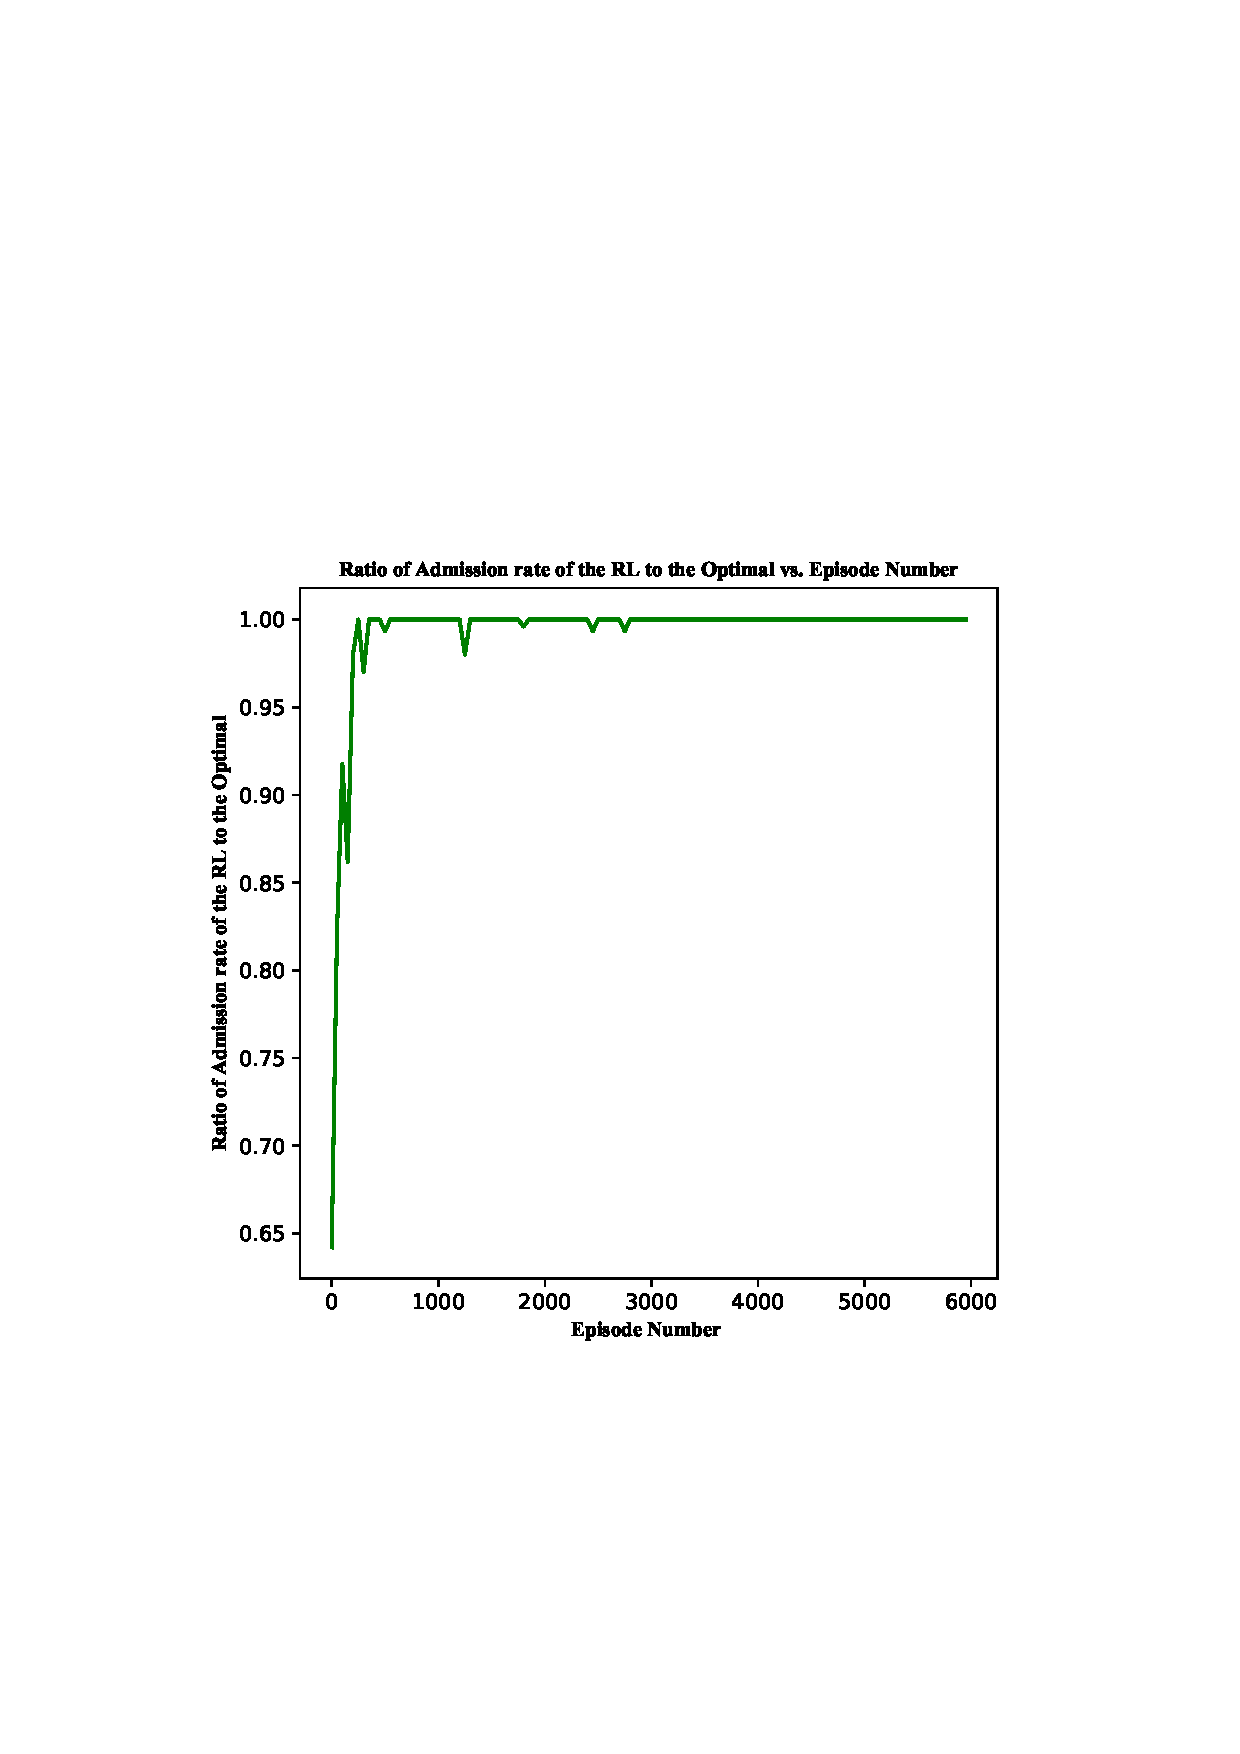
\includegraphics[scale = 0.6]{./fig/dynamicEpoch_0} %[width=\linewidth] 
	\caption{  نسبت تعداد سرویسهای پذیرفته شده با استفاده از روش یادگیری تقویتی عمیق به نسبت تعداد سرویسهای پذیرفته شده در حالت بهینه براساس زمان طی شده}
	\label{fig:dynamicEpoch}
\end{figure}
در شکل \ref{fig:dynamicEpoch1}
با افزایش تعداد برشها و بیشینه تعداد درخواستها در هر زمان، بعد از 1000 تکرار سناریو جواب به حالت بهینه نزیک شده ولی هیچ موقع با مقدار بهینه برابری نمی‌کند. در اینجا، تعداد درخواستهای سرویس اول 10 تا و سرویس دوم 5 تا می‌باشد. همچنین نرخ خروج نرخ  در هر بازه‌ی زمانی $80$ درصد فرض شده است.% در اینجا هر سناریو 100 بار تکرار شده و میانگین گیری برروی آن انجام گردیده است.
\begin{figure}%[H]
	\centering
	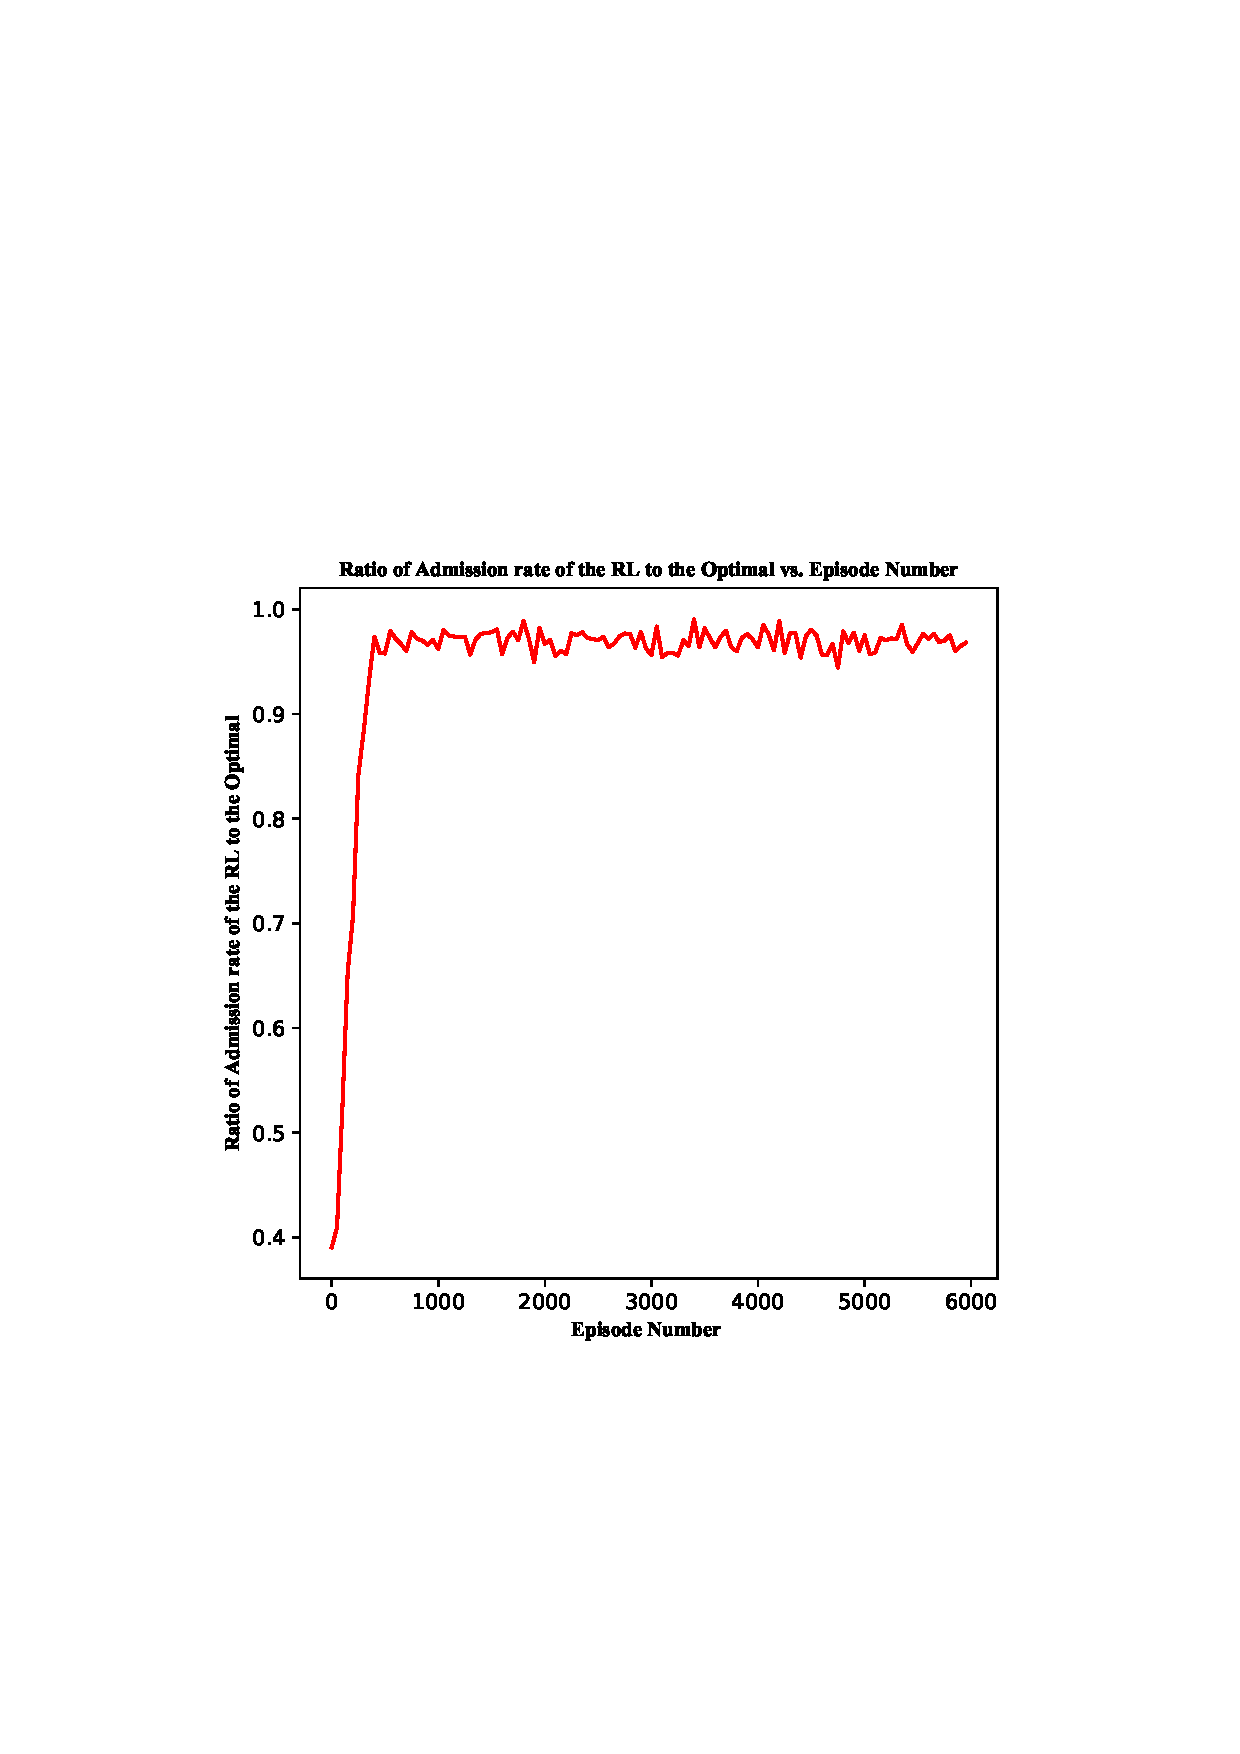
\includegraphics[scale = 0.6]{./fig/dynamicEpoch1_0} %[width=\linewidth] 
	\caption{  نسبت تعداد سرویسهای پذیرفته شده روش استفاده شده به نسبت تعداد سرویسهای پذیرفته شده در حالت بهینه براساس زمان طی شده با افزایش تعداد ماکسیمم درخواستها و تعداد برشهای شبکه}
	\label{fig:dynamicEpoch1}
\end{figure}
\subsection{نتایج عددی مسئله‌ی دوم} 
در این بخش، برای مسئله‌ی دوم حالت، عامل و پاداش را تعیین می‌نماییم و سپس نتایج عملی را نشان می‌دهیم.
در این مسئله، عامل، orchestrator است که وظیفه‌ی مدیریت شبکه را برعهده دارد.
همچنین، حالت در هر بازه‌ی زمانی برشهایی از شبکه است که به مراکزداده متصل شده و اینکه کدام برش به کدام مرکز داده متصل است.
پاداش طوری تعیین شده که کمترین تعداد مراکز داده استفاده گردد و هر لحظه کمترین تعداد مرکز داده‌ی خاموش، روشن شود.
در اینجا با فرض داشتن دو مدل سرویس مسئله را شبیه سازی می کنیم. فرض کنید VNF های سرویس اول نیاز به 
\lr{1 CPU}
و سرویس دوم نیازمند 
\lr{2 CPU}
است.
فرض کنید از سرویس اول ماکسیمم 6 تا درخواست VNF 
و برای سرویس دوم ماکسیمم در هر لحظه‌ی زمانی 4 تا درخواست VNF صورت می‌گیرد.
در این مسئله، تعداد زیادی سرور که دارای 3 تا CPU هستند در نظر گرفته شده است.
نسبت تعداد سرورهای مصرفی بهینه به سرورهای مصرفی با روش Q-learning  در شکل
\ref{fig:dynamicEpoch2}
نشان داده شده است.
\begin{figure}%[H]
	\centering
	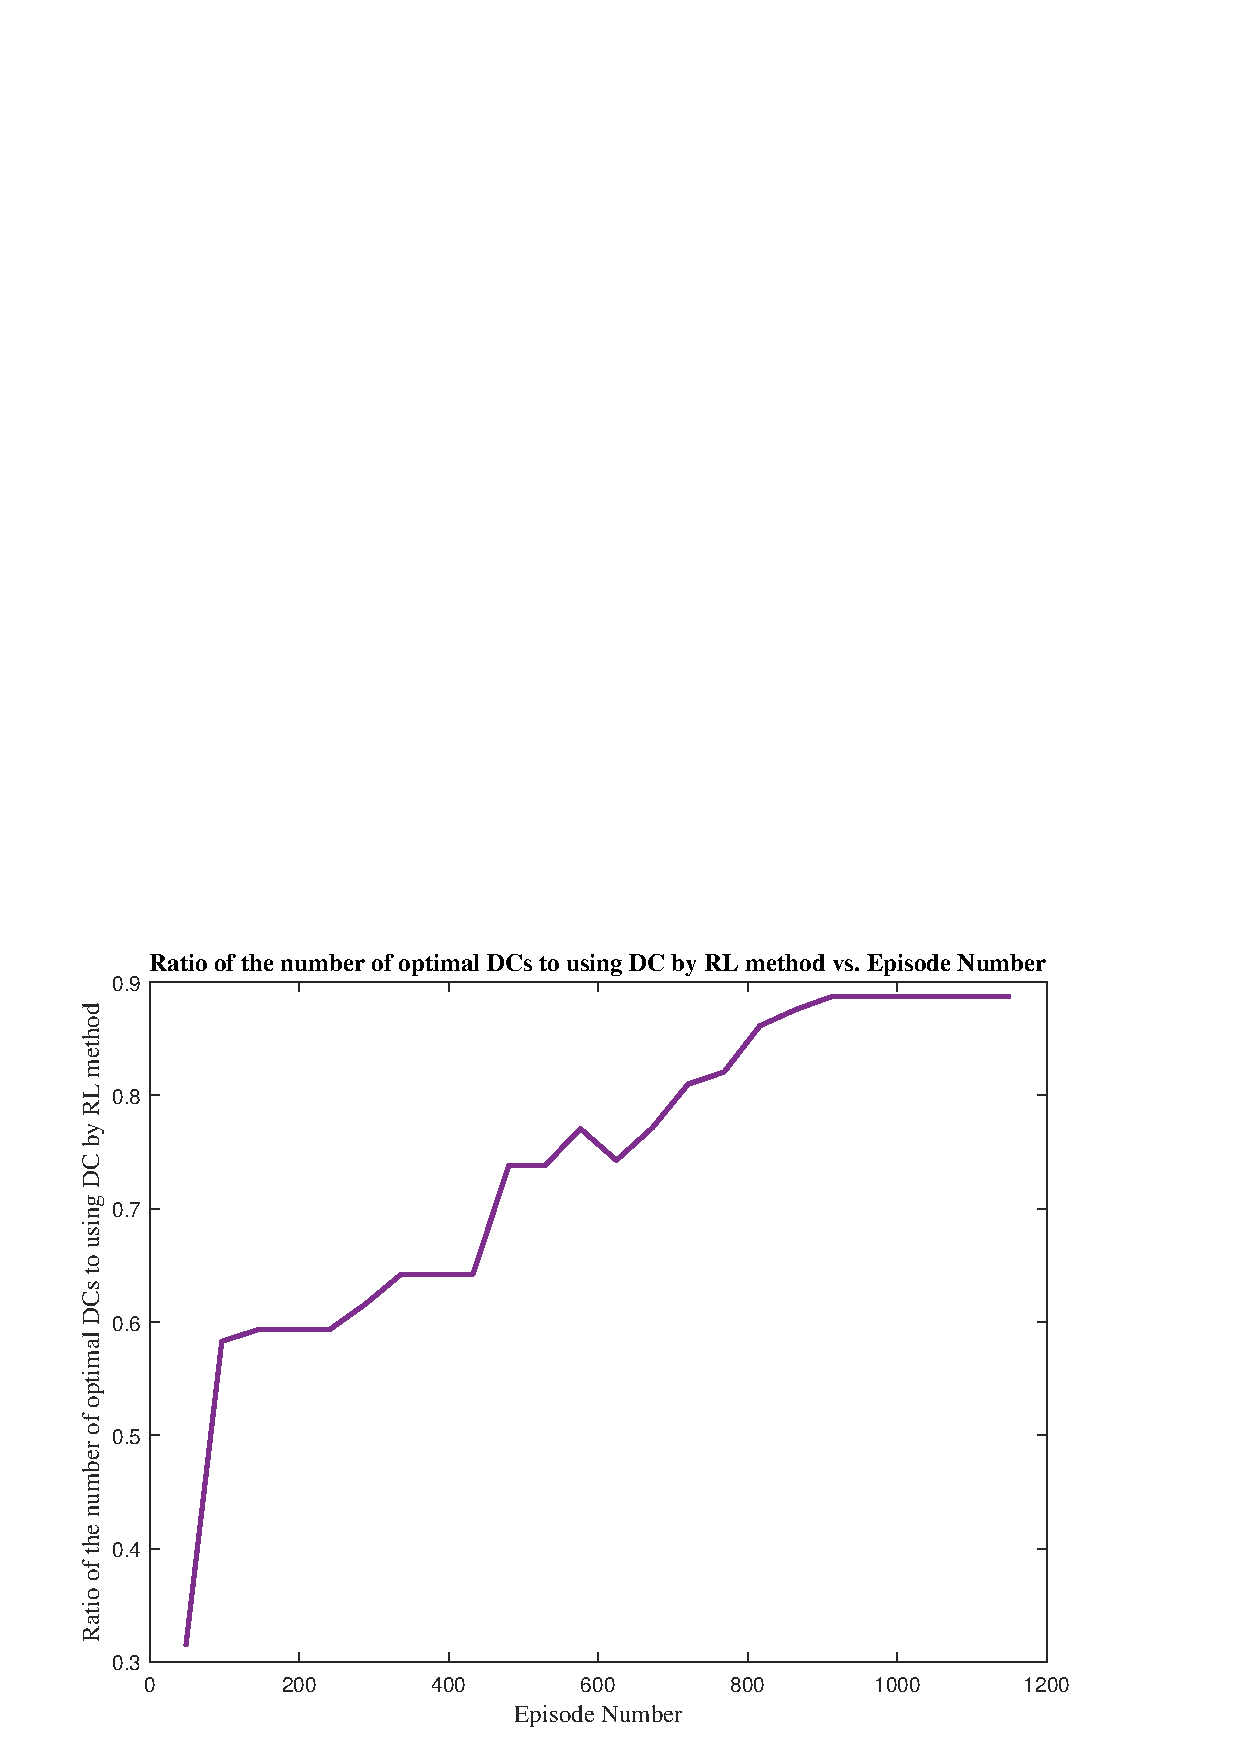
\includegraphics[scale = 0.6]{./fig/ratio_episode2} %[width=\linewidth] 
	\caption{   نسبت تعداد سرورهای مصرفی با روش 
		بهینه
		 به سرورهای مصرفی با استفاده از روش یادگیری تقویتی براساس زمان طی شده}
	\label{fig:dynamicEpoch2}
\end{figure}
همانطور که دیده می‌شود بعد از 900
تا تکرار، تقریبا به مقدار بهینه با نسبت $0.9$ نزدیک شده‌ایم.
بعد از 900 تا تکرار سناریو، تقریبا میزان انتخاب عمل رندم به صفر رسیده و عمل بهینه از روی جدول Q بدست می‌آید.
%در اینجا هر سناریو 100 بار تکرار شده و میانگین گیری برروی آن انجام گردیده است. 
نرخ خروج در هر بازه‌ی زمانی $80$ درصد فرض شده است.
\section{نتیجه‌گیری}
در این فصل، دو مسئله‌ی فصل قبلی به صورت ساده شده نوشته شد و مسئله‌ی اول در بخش رادیویی از جنس کوله‌پشتی و مسئله‌ی دوم در بخش هسته از نوع 
بسته‌بندی جعبه می‌باشد. این دو مسئله به صورت دینامیکی در هر لحظه از زمان حل شده‌اند. برای حل این دو مسئله از روش یادگیری تقویتی  استفاده شده و حالتها و اعمال بیان برای یک عامل در این مسئله بیان گرده است.
نتایج عملی آن نیز رسم گردید. در هردو مسئله‌، به دلیل گسسته بودن اعمال و حالات مسئله و کم بودن تعداد آن از روش Q-learning
استفاده نمودیم. در مسئله‌ی اول ابتدا با فرض تعداد کمتر مسئله بعد از تعدادی تکرار به مقدار بهینه می‌رسد. با افزایش درخواستها از مقدار بهینه تا حدی دور می‌گردد. در مسئله‌ی دوم نیز بعد از 900 تکرار و با استفاده از جدول Q به مقدار نسبتا بهینه میل می‌کند.

  		% فصل چهارم: نتایج
\chapter{پیشنهادات و کارهای آتی}
\section{مقدمه}
در فصل اول، مقدمه‌ای بر مفاهیم مورد استفاده را بیان کردیم و در مورد نسل پنجم مخابرات و مفاهیم آن صحبت نمودیم. سپس در فصل دوم مروری بر کارهای انجام شده کردیم و مقالات مرتبط با برش شبکه و شبکه‌های دسترسی باز و قرارگیری توابع مجازی شبکه را بیان نمودیم تا مروری بر چالشهای مطرح شده نسل پنجم مخابرات کرده و حل این چالشها را مورد بررسی قرار دادیم . در فصل سوم صورت مسئله‌ای در زمینه‌ی برش شبکه در شبکه‌های دسترسی باز، معرفی کرده و با روش ابتکاری، آن را حل نمودیم و نتایج را با مقدار بهینه مقایسه کردیم.
در  فصل چهارم، دو مسئله‌ی بیان شده در فصل سوم را به صورت کاملا ساده با روش یادگیری عمیق تقویتی به صورت دینامیکی و در هر بازه‌ی زمان حل نمودیم. این دو مسئله، MDP \LTRfootnote{Markov Decision Processs}
بوده و قابل حل با این روش هستند. 
حال در این فصل در مورد مزایا و معایب کارهای انجام شده در فصل سوم و چهارم صحبت کرده و کارهای آتی و پیشنهادات را بیان می‌کنیم.
\section{نتیجه‌گیری}
در اینجا، مسئله‌ی برش شبکه در بخش رادیویی و قرارگیری توابع مجازی شبکه برروی مراکز داده باهم مورد بررسی قرار گرفته شد.
برای حل این مسئله، ابتدا مسئله به دو بخش مختلف شکسته شد که در بخش اول، تخصیص برش شبکه به کاربران سرویسها و تخصیص توان حل شده و پس از آن، برشهایی از شبکه که به سرویس اختصاص داده شده را به مراکز داده نگاشت می‌دهیم.
در این مسئله، تاخیر و نرخ هر کاربر در سرویس مورد بررسی قرار گرفته شده و چالش تخصیص منابع که شامل برش بخش رادیویی به هر سرویس است و جاگیری توابع شبکه حل می‌شود.
 الگوریتم ارائه شده سرعت بسیار بیشتری از الگوریتم بهینه که با MOSEK و CVX بدست می‌آید، دارد.
 سپس مسئله به صورت ساده‌تر برای حالت دینامیکی با روش یادگیری تقویتی حل گردیده است. 
 \subsection{مزایای این چالش و حل آن}
 در مسئله‌ی بیان شده‌ی فصل سوم، مدل سیستم به صورت دقیق بیان شده و نرخ کاربر، ظرفیت لینک fronthaul و تاخیر به طور دقیق مورد بررسی قرار گرفته شده است. همچنین مسئله به واقعیت نزدیکی زیادی دارد. همچنین الگوریتم ابتکاری تعریف شده در فصل سوم برای حالتی که تداخل به نسبت کم باشد به حالت بهینه بسیار نزدیک است. در فصل چهارم همین مسئله با فرض اینکه سرویسها نیازمند تاخیر کم یا نرخ بالا هستند به صورت پارامتریک در هر لحظه از زمان حل می‌گردند. 
 در بخش بعدی چالشهای قرارگیری توابع مجازی برروی مراکز داده به طور دقیق بررسی شده و ‌در فصل چهارم این مسئله به صورت دینامیکی در هر لحظه حل گردیده است. در حل مسئله در حالت دینامیکی سعی براین است که مراکز داده کمترنی انرژی را مصرف نموده و از هدر رفت انرژی بپرهیزیم.
 \subsection{معایب  پروژه انجام شده}
 در فصل سوم از الگوریتم ابتکاری در این کار استفاده شده است. زمانی که تعداد بلوکهای منابع فیزیکی به نسبت کاربران بسیار کم باشد و تداخل به شدت زیاد گردد، الگوریتم مسئله‌ی اول به خوبی قادر به پاسخ‌گویی نیست و از حالت بهینه فاصله ‌می‌گردد. در مسئله‌ی دوم، زمانی که تعداد مراکز داده زیاد گردد فاصله‌ی حالت بهینه از الگوریتم ابتکاری زیاد شده است. 
همچنین در فصل چهارم صورت مسئله بسیار ساده‌تر از واقعیت است و مسئله در حالت دینامیکی برای تعداد درخواست کم در این حالت حل گردیده است.
 \subsection{نوآوری‌های این پروژه}
 در این پروژه، تخصیص توان و برش شبکه در شبکه‌های دسترسی باز مورد بررسی قرار گرفته است.
 ما مسئله‌ی اختصاص UE به خدمات، خدمات به برش‌ها و منابع فیزیکی بی سیم و همچنین مرکز داده به برش‌ها را به عنوان یک مشکل بهینه سازی فرمول‌بندی کرده‌ایم. سپس با ارائه‌ی روشهای ابتکاری، به حل آنها پرداختیم. در نهایت مسئله‌ی ساده شده را در حالت دینامیکی و متغیر با زمان حل کردیم.
 \section{پیشنهادات}
 در این بخش، پیشنهادات و کارهای آتی را بیان خواهیم کرد.
 \begin{itemize}
\item
 یکی از کارهای آتی، مدل کردن برش شبکه در ساختار شبکه‌ی دسترسی رادیویی باز و حل آن بوسیله‌ی روش یادگیری تقویتی عمیق می‌باشد. در فصل چهارم از این روش برای سیستم ساده شده استفاده گردیده و به دلیل کم بودن تعداد حالات با استفاده از روش یادگیری تقویتی حل شده و در فصل سوم نیز مدل سیستم بیان شده، یکی از کارهای بعدی این است که سیستم مدل فصل سوم را به سیستمهای رادیویی باز نزدیکتر کرده و
با روش یادگیری تقویتی عمیق حل نماییم. که در اینجا، بدست آوردن توان و ارتباط برش با سرویس از این روش بدست خواهد آمد. همچنین مقایسه‌ی روش یادگیری تقویتی عمیق و یادگیری تقویتی در اینجا نیز مورد توجه قرار خواهد گرفت.
\item 
یکی دیگر از کارهای آتی، بدست آوردن پارامترهای کیفیت سرویس QoS\LTRfootnote{Quality of Service}
در شبکه‌های دسترسی باز می‌باشد که شامل تاخیر انتها به انتها، میزان از دست دادن بسته ها\LTRfootnote{Packet Loss}،
قابلیت اطمینان و ... می‌باشد.
در اینجا می‌توان تاخیر را هم در بخش رادیویی هم در بخش هسته‌ی شبکه بدست آورد. 
همچنین،
به منظور نشان دادن نقش هوش در ORAN طرح مدیریت هوشمند منابع رادیویی را برای کنترل تراکم ترافیک و نشان دادن کارایی آن در یک مجموعه داده واقعی از یک اپراتور بزرگ بدست می‌آوریم.
\item 
شبکه تعریف شده توسط نرم افزار (SDN) و مجازی سازی عملکرد شبکه (NFV) فناوری های کلیدی امکان پذیر در شبکه های ارتباطی نسل پنجم (5G) برای قرارگیری برش های شبکه سفارشی در سطح سرویس در زیرساخت شبکه، بر اساس خواسته های منابع آماری برای تأمین کیفیت طولانی مدت خدمات (QoS) مورد نیاز می‌باشد. با این حال، بارهای ترافیکی در برش های مختلف با گذشت زمان تحت تغییر قرار می‌گیرند ، در نتیجه چالش هایی برای تأمین کیفیت کیفیت مداوم ایجاد می‌شود.
در کارهای آتی یک مشکل انتقال جریان پویا برای سرویس های متصل شده به برش شبکه، برای پاسخگویی به نیازهای تأخیر پایان انتها به انتها (E2E) با ترافیک متغیر، مورد بررسی قرار خواهد گرفت.
\item
یکی دیگر از کارهای آتی، تخصیص منابع به روش توزیع شده برای برش شبکه از منابع محاسباتی و منابع دیگر همانند پهنای باند می‌باشد.
همچنین از روش توزیع شده در لینک فراسو  
\LTRfootnote{Uplink}
برای تخصیص توان کاربران، تخصیص پهنای باند و ... استفاده می‌گردد. یکی از روشها، استفاده از 
\lr{Distributed ADMM}
می‌باشد که در این روش تعدادی عامل به صورت همکارانه سعی در حل یک معادله‌ی بهینه‌سازی مشترک دارند که تابع هدف مجموعی از مقدارهای خصوصی هر عامل ‌می‌باشد. 
 \end{itemize}
 
  		% فصل پنجم: بحث و نتیجه‌گیری

% مراجع
% اگر از استیل‌های natbib استفاده می‌کنید باید دو خط را در فایل commands.tex تغییر دهید.
\pagestyle{empty}
{
\small
\onehalfspacing
%\bibliographystyle{plain-fa} % or plainnat-fa for author-date


\begin{latin}
\bibliographystyle{IEEEtran}
\renewcommand{\bibname}{\rl{{کتاب‌نامه}\hfill}} 
\bibliography{./tex/MyReferences}
\end{latin}
}

\pagestyle{fancy}

% \appendix
% فصلهای پس از این قسمت به عنوان ضمیمه خواهند آمد.

% دستورات لازم برای تبدیل «فصل آ» به «پیوست آ» در فهرست مطالب 
\addtocontents{toc}{
    \protect\renewcommand\protect\cftchappresnum{\appendixname~}%
    \protect\setlength{\cftchapnumwidth}{\mylenapp}}
    
\let\Chapter\chapter
% دستورات لازم برای شماره‌گذاری صفحات پیوست‌ها بشکل آ-۱ (فعلا با glossaries سازگار نیست)
%\pretocmd{\chapter}{
%  \clearpage
%  \pagenumbering{arabic}
%  \renewcommand*{\thepage}{\rl{\thechapter-\arabic{page}}}}{}{}
%%%%%%%%%%%%%%%%%%%%%%%%%%%%%%%%%%%%%
    

% !TeX root=../main.tex

\chapter{آشنایی سریع با برخی دستورات لاتک}
\label{app:latexIntro}
%\thispagestyle{empty}
در این فصل ویژگی‌های مهم و پرکاربرد زی‌پرشین و لاتک معرفی می‌شود. برای راهنمایی بیشتر و به‌کاربردن ویژگی‌های پیشرفته‌تر به راهنمای زی‌پرشین و راهنمای لاتک مراجعه کنید. برای آگاهی از دستورات لاتک که این خروجی را تولید کرده‌اند فایل \lr{appendix1.tex} را ملاحظه فرمایید.
\footnote{بیشتر مطالب این بخش از مثال 
\lr{xepersian\_example.tex}
گرفته شده‌اند که توسط آقای امیرمسعود پورموسی آماده شده است.}

\section{بندها و زیرنویس‌ها}
هر جایی از نوشتهٔ خود، اگر می‌خواهید به سر سطر بروید و یک بند (پاراگراف) تازه را آغاز کنید، باید یک خط را خالی بگذارید%
\footnote{یعنی دوبار باید کلید \lr{Enter} را بزنید.}
 مانند این:

حالا که یک بند تازه آغاز شده است، یک زیرنویس انگلیسی%
\LTRfootnote{English Footnote!}
 هم می‌نویسیم!
\section{فرمول‌های ریاضی}
\label{formula}

اینجا هم یک فرمول می‌آوریم که شماره دارد:
\begin{equation}\label{eq:yek}
A=\frac{c}{d}+\frac{q^2}{\sin(\omega t)+\Omega_{12}}
\end{equation}
در لاتک می‌توان به کمک فرمان 
\lr{\textbackslash label\{\}}
به هر فرمول یک نام نسبت داد. در فرمول بالا نام \lr{eq:yek} را برایش گذاشته‌ایم (پروندهٔ \lr{tex} همراه با این مثال را ببینید). این نام ما را قادر می‌کند که بعداً بتوانیم با فرمان
\lr{\textbackslash ref\{eq:yek\}}
به آن فرمول با شماره ارجاع دهیم. یعنی بنویسیم فرمول \ref{eq:yek}. 
لاتک خودش شمارهٔ این فرمول‌ها را مدیریت می‌کند.\footnote{یعنی اگر بعداً فرمولی قبل از این فرمول بنویسیم، خودبه‌خود شمارهٔ این فرمول و شمارهٔ ارجاع‌ها به این فرمول یکی زیاد می‌شود. دیگر نگران شماره‌گذاری فرمول‌های خود نباشید!} این هم یک فرمول که شماره ندارد:
$$A=|\vec{a}\times \vec{b}| + \sum_{n=0}^\infty C_{ij}$$

این هم عبارتی ریاضی مانند 
$\sqrt{a^2+b^2}$
 که بین متن می‌آید.
\subsection{یک زیربخش}
\label{zirbakhsh}

این زیربخش \ref{zirbakhsh} است؛ یعنی یک بخش درون بخش \ref{formula} است.
\subsubsection{یک زیرزیربخش}
این هم یک زیرزیربخش است. در لاتک می‌توانید بخش‌های تودرتو در نوشته‌تان تعریف کنید تا ساختار منطقی نوشته را به خوبی نشان دهید. می‌توانید به این بخش‌ها هم با شماره ارجاع دهید، مثلاً بخش فرمول‌های ریاضی شماره‌اش \ref{formula} است.
\section{نوشته‌های فارسی و انگلیسی مخلوط}
نوشتن یک کلمهٔ انگلیسی بین متن فارسی بدیهی است، مانند Example در این جمله.\footnote{هرچند بهتر است باز هم آن کلمه را مانند \lr{Example} در این جمله بنویسید.}
نوشتن یک عبارت چندکلمه‌ای مانند
 \lr{More than one word} کمی پیچیده‌تر است.

اگر ناگهان تصمیم بگیرید که یک بند کاملاً انگلیسی را بنویسید، باید:
\begin{latin}
This is an English paragraph from left to right. You can write as much as you want in it.
\end{latin}
\section{افزودن تصویر به نوشته}
پروندهٔ تصویر دلخواه خود را در کنار پروندهٔ \lr{tex} قرار دهید. سپس به روش زیر تصویر را در نوشتهٔ خود بیاورید:
\begin{latin}
\begin{verbatim}
\includegraphics{YourImageFileName}
\end{verbatim}
\end{latin}
به تصویرها هم مانند فرمول‌ها و بخش‌ها می‌توان با شماره ارجاع داد. مثلاً تصویر \ref{fig:shir} یک شیر علاقه‌مند به لاتک را در حال دویدن نشان می‌دهد. برای جزئیات بیشتر دربارهٔ روش گذاشتن تصویرها در نوشته باید راهنماهای لاتک را بخوانید.
\begin{figure}[ht]
\centerline{
\includegraphics[width=5cm]{lion}}
\caption{در این تصویر یک شیر علاقه‌مند به لاتک را در حال دویدن می‌بینید.}
\label{fig:shir}
\end{figure}

به تصویرها هم مانند فرمول‌ها و بخش‌ها می‌توان با شماره ارجاع داد. مثلاً تصویر بالا شماره‌اش \ref{fig:shir} است. برای جزئیات بیشتر دربارهٔ روش گذاشتن تصویرها در نوشته باید راهنماهای لاتک را بخوانید.

\section{محیط‌های شمارش و نکات}
برای فهرست‌کردن چندمورد، اگر ترتیب برایمان مهم نباشد:
\begin{itemize}
\item مورد یکم
\item مورد دوم
\item مورد سوم
\end{itemize}
و اگر ترتیب برایمان مهم باشد:
\begin{enumerate}
\item مورد یکم
\item مورد دوم
\item مورد سوم
\end{enumerate}
می‌توان موردهای تودرتو داشت:
\begin{enumerate}
\item مورد ۱
\item مورد ۲
\begin{enumerate}
\item مورد ۱ از ۲
\item مورد ۲ از ۲
\item مورد ۳ از ۲
\end{enumerate}
\item مورد ۳
\end{enumerate}
شماره‌گذاری این موردها را هم لاتک انجام می‌دهد.

\section{تعریف و قضیه}
برای ذکر تعریف، قضیه و مثال مثالهای ذیل را ببینید.
\begin{definition}
مجموعه همه ارزیابی‌های  (پیوسته)  روی $(X,\tau)$، دامنه توانی احتمالی
\index{دامنه توانی احتمالی}
$ X $
نامیده می‌شود.
\end{definition}
\begin{theorem}[باناخ-آلااغلو]
\index{قضیه باناخ-آلااغلو}
اگر $ V $ یک همسایگی $ 0 $ در فضای برداری 
\index{فضای!برداری}
 توپولوژیکی $ X $ باشد و 
\begin{equation}\label{eq1}
K=\left\lbrace \Lambda \in X^{*}:|\Lambda x|\leqslant 1 ; \ \forall x\in V\right\rbrace,
\end{equation}
آنگاه $ K $،  ضعیف*-فشرده است که در آن، $ X^{*} $ دوگان
\index{فضای!دوگان}
 فضای برداری توپولوژیکی $ X $ است به ‌طوری که عناصر آن،  تابعی‌های 
خطی پیوسته
\index{تابعی خطی پیوسته}
 روی $X$ هستند.
\end{theorem}
تساوی \eqref{eq1} یکی از مهم‌ترین تساوی‌ها در آنالیز تابعی است که در ادامه، به وفور از آن استفاده می‌شود.
\begin{example}
برای هر فضای مرتب، گردایه 
$$U:=\left\lbrace U\in O: U=\uparrow U\right\rbrace $$
از مجموعه‌های بالایی باز، یک توپولوژی تعریف می‌کند که از توپولوژی اصلی، درشت‌تر  است.
\end{example}
حال تساوی 
\begin{equation}\label{eq2}
\sum_{n=1}^{+\infty} 3^{n}x+7x=\int_{1}^{n}8nx+\exp{(2nx)}
\end{equation}
را در نظر بگیرید. با مقایسه تساوی \eqref{eq2} با تساوی \eqref{eq1} می‌توان نتیجه گرفت که ...


\section{چگونگی نوشتن و ارجاع به مراجع}
\label{Sec:Ref}


در لاتک به راحتی می‌توان مراجع خود را نوشت و به آنها ارجاع داد. به عنوان مثال برای معرفی کتاب گنزالس \cite{Gonzalez02book} به عنوان یک مرجع می‌توان آنرا به صورت زیر معرفی نمود:

\singlespacing
\begin{LTR}
\begin{verbatim}
\bibitem{Gonzalez02book}
Gonzalez, R.C., and Woods, R.E. {\em Digital Image Processing}, 3rd ed..
Prentice-Hall, Inc., Upper Saddle River, NJ, USA, 2006.
\end{verbatim}
\end{LTR}
\doublespacing

در دستورات فوق \lr{Gonzalez02book}  برچسبی است که به این مرجع داده شده است و با استفاده از دستور 
\verb!\cite{Gonzalez02book}!
می‌توان به آن ارجاع داد؛ بدون این که شماره‌اش را در فهرست مراجع‌مان بدانیم.

اگر این اولین مرجع ما باشد در قسمت مراجع به صورت زیر خواهد آمد:\\
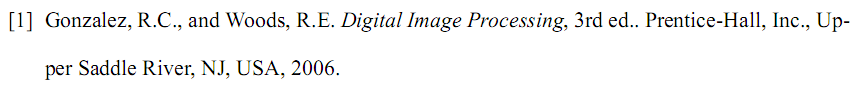
\includegraphics[width=\textwidth]{gonzalez.png}

این شیوهٔ تعریف مراجع بسیار ابتدایی است و اگر فرمت مراجع، ترتیب یا تعداد آنها را خواسته باشید تغییر دهید، به عنوان مثال ابتدا حرف اول نام نویسنده بیاید و سپس نام خانوادگی، باید همه کارها را به صورت دستی انجام دهید!
چون در یک \پ یا مقاله باید کنترل کاملی بر مراجع خود داشته باشید و به راحتی بتوانید قالب مراجع را عوض کنید، بنابراین می‌بایست از \lr{Bib\TeX} استفاده کنید که درپیوست  \ref{app:refMan} به  آن پرداخته خواهد شد.
		% پیوست اول: آشنایی مقدماتی با لاتک
% !TeX root=../main.tex

\chapter{‌جدول، نمودار و الگوریتم در لاتک}
\label{app:latex:more}
%\thispagestyle{empty}

در این بخش نمونه مثالهایی از جدول، شکل، نمودار، الگوریتم و معادلات ریاضی را در لاتک خواهیم دید.
دقت کنید که در پایان‌نامه‌ها و مقالات، باید قاعدهٔ «ارجاع به جلو%
\LTRfootnote{Forward Referencing}»
رعایت شود؛ یعنی ابتدا در متن به شمارهٔ شکل، جدول یا معادله اشاره شود و بعد از آن (زیر آن) خود شکل، جدول یا معادله رسم شود. (توضیحات بیشتر در قسمت
\ref{sec:floatObjs}).

\section{جدول}
دستور اصلی برای رسم جدول در لاتک 
\verb|tabular|
می‌باشد که جدول
\eqref{tab:motionModels}
با استفاده از آن کشیده شده است؛ در
\verb|tabular|
عرض جدول برابر با مجموع عرض ستون‌ها و حداکثر مساوی عرض متن است.
\begin{table}[ht]
\caption{مدلهای تبدیل.}
\label{tab:motionModels}
\centering
\onehalfspacing
\begin{tabular}{|r|c|l|r|}
	\hline نام مدل & درجه آزادی & تبدیل مختصات & توضیح \\ 
	\hline انتقالی & ۲ & $\begin{aligned} x'=x+t_x \\ y'=y+t_y \end{aligned}$  &  انتقال دوبعدی\\ 
	\hline اقلیدسی & ۳ & $\begin{aligned} x'=x\cos\theta - y\sin\theta+t_x \\ y'=x\sin\theta+y\cos\theta+t_y \end{aligned}$  &  انتقالی+دوران \\ 
	\hline 
\end{tabular} 
\end{table}

برای اینکه عرض جدول قابل کنترل باشد، باید از دستورات
\verb|tabularx|،
\verb|tabulary| یا
\verb|tabu|
استفاده کرد که راهنمای آنها در اینترنت وجود دارد.
مثلاً جدول
\ref{tab:motionModelsCont}
با
\verb|tabularx|
رسم شده که عرض جدول در آن ثابت بوده و ستون‌های از نوع
\verb|X|
عرض خالی جدول را پر می‌کنند.
\begin{table}[ht]
	\caption{مدلهای تبدیل دیگر.}
	\label{tab:motionModelsCont}
	\centering
	\onehalfspacing
	\begin{tabularx}{\textwidth}{|r|c|l|X|}
		\hline نام مدل & درجه آزادی & تبدیل مختصات & توضیح \\ 
		\hline مشابهت & ۴ & $\begin{aligned} x'=sx\cos\theta - sy\sin\theta+t_x \\ y'=sx\sin\theta+sy\cos\theta+t_y  \end{aligned}$  & اقلیدسی+تغییرمقیاس \\ 		
		\hline آفین & ۶ & $\begin{aligned} x'=a_{11}x+a_{12}y+t_x \\ y'=a_{21}x+a_{22}y+t_y \end{aligned}$  & مشابهت+اریب‌شدگی \\
		\hline
	\end{tabularx}
\end{table}

\section{معادلات ریاضی و ماتریس‌ها}
تقریباً هر آنچه دانشجویان برای نوشتن فرمول‌های ریاضی لازم دارند، در کتاب 
\lr{mathmode}
آمده است. کافیست در خط فرمان، دستور زیر را وارد کنید:
\begin{latin}
	\texttt{texdoc mathmode}
\end{latin}
متن زیر شامل انواعی از اشیاء ریاضی است که با ملاحظه کدش می‌توانید با دستورات آن آشنا شوید.\\
شناخته‌شده‌ترین روش تخمین ماتریس هوموگرافی الگوریتم تبدیل خطی مستقیم (\lr{DLT\LTRfootnote{Direct Linear Transform}}) است.  فرض کنید چهار زوج نقطهٔ متناظر در دو تصویر در دست هستند،  $\mathbf{x}_i\leftrightarrow\mathbf{x}'_i$   و تبدیل با رابطهٔ
  $\mathbf{x}'_i = H\mathbf{x}_i$
  نشان داده می‌شود که در آن:
\[\mathbf{x}'_i=(x'_i,y'_i,w'_i)^\top  \]
و
\[ H=\left[
\begin{array}{ccc}
h_1 & h_2 & h_3 \\ 
h_4 & h_5 & h_6 \\ 
h_7 & h_8 & h_9
\end{array} 
\right]\]
رابطه زیر را برای الگوریتم  \eqref{alg:DLT} لازم داریم.
\begin{equation}
\label{eq:DLT_Ah}
\left[
\begin{array}{ccc}
	0^\top & -w'_i\mathbf{x}_i^\top & y'_i\mathbf{x}_i^\top \\ 
	w'_i\mathbf{x}_i & 0^\top & -x'_i\mathbf{x}_i^\top \\ 
	- y'_i\mathbf{x}_i^\top & x'_i\mathbf{x}_i^\top & 0^\top
\end{array} 
\right]
\left(
\begin{array}{c}
	\mathbf{h}^1 \\ 
	\mathbf{h}^2 \\ 
	\mathbf{h}^3
\end{array} 
\right)=0
\end{equation}

\section{الگوریتم با دستورات فارسی}
با مفروضات فوق، الگوریتم \lr{DLT} به صورت نشان داده شده در الگوریتم \eqref{alg:DLT}  خواهد بود.
\begin{algorithm}[ht]
\onehalfspacing
\caption{الگوریتم \lr{DLT} برای تخمین ماتریس هوموگرافی.} \label{alg:DLT}
\begin{algorithmic}[1]
\REQUIRE $n\geq4$ زوج نقطهٔ متناظر در دو تصویر 
${\mathbf{x}_i\leftrightarrow\mathbf{x}'_i}$،\\
\ENSURE ماتریس هوموگرافی $H$ به نحوی‌که: 
$\mathbf{x}'_i = H \mathbf{x}_i$.
  \STATE برای هر زوج نقطهٔ متناظر
$\mathbf{x}_i\leftrightarrow\mathbf{x}'_i$ 
ماتریس $\mathbf{A}_i$ را با استفاده از رابطهٔ \ref{eq:DLT_Ah} محاسبه کنید.
  \STATE ماتریس‌های ۹ ستونی  $\mathbf{A}_i$ را در قالب یک ماتریس $\mathbf{A}$ ۹ ستونی ترکیب کنید. 
  \STATE تجزیهٔ مقادیر منفرد \lr{(SVD)}  ماتریس $\mathbf{A}$ را بدست آورید. بردار واحد متناظر با کمترین مقدار منفرد جواب $\mathbf{h}$ خواهد بود.
  \STATE  ماتریس هوموگرافی $H$ با تغییر شکل $\mathbf{h}$ حاصل خواهد شد.
\end{algorithmic}
\end{algorithm}

\section{الگوریتم با دستورات لاتین}
الگوریتم \ref{alg:RANSAC} یک الگوریتم با دستورات لاتین است.

\begin{algorithm}[ht]
\onehalfspacing
\caption{الگوریتم \lr{RANSAC} برای تخمین ماتریس هوموگرافی.} \label{alg:RANSAC}
\begin{latin}
\begin{algorithmic}[1]
\REQUIRE $n\geq4$ putative correspondences, number of estimations, $N$, distance threshold $T_{dist}$.\\
\ENSURE Set of inliers and Homography matrix $H$.
\FOR{$k = 1$ to $N$}
  \STATE Randomly choose 4 correspondence,
  \STATE Check whether these points are colinear, if so, redo the above step
  \STATE Compute the homography $H_{curr}$ by DLT algorithm from the 4 points pairs,
  \STATE $\ldots$ % الگوریتم کامل نیست
  \ENDFOR
  \STATE Refinement: re-estimate H from all the inliers using the DLT algorithm.
\end{algorithmic}
\end{latin}
\end{algorithm}

\section{درج کد}
درج کد به زبان‌های مختلف به سادگی امکان‌پذیر است. برنامه
\ref{code:matlabEx}
یک قطعه کد
\lr{MATLAB}
را نشان می‌دهد.
\singlespacing
\begin{figure}
	\begin{LTR}
		\lstinputlisting[language=MATLAB, caption={نمونه کد \lr{MATLAB}}, label={code:matlabEx}]{MatlabExample.m}
	\end{LTR}
\end{figure}
\doublespacing

\section{تصویر}
نمونهٔ یک تصویر را در فصل قبل دیدیم. دو تصویر شیر کنار هم را نیز در شکل
\ref{fig:twoLion}
مشاهده می‌کنید.
\begin{figure}[ht]
\centering 
\subfloat[شیر ۱]{ \label{fig:twolion:one}

\includegraphics[width=0.3\textwidth]{lion}}
%\hspace{2mm}
\subfloat[شیر ۲]{ \label{fig:twolion:two}

\includegraphics[width=0.3\textwidth]{lion}}%
\caption{دو شیر}
\label{fig:twoLion} %% label for entire figure
\end{figure}

\section{نمودار}
لاتک بسته‌هایی با قابلیت‌های زیاد برای رسم انواع مختلف نمودارها دارد. مانند بسته‌های \lr{Tikz} و  \lr{PSTricks}. توضیح اینها فراتر از این پیوست کوچک است.%
\footnote{
مثال‌هایی از بکارگیری بسته
\lr{Tikz}
را می‌توانید در
\url{http://www.texample.net/tikz/examples/}
ببینید. توصیه می‌شود دانشجویانی که قصد درج اشکالی مانند گراف را در سند خود دارند، مثالهایی از سایت مذکور را ملاحظه فرمایند.
}
یک نمودار رسم شده با بسته‌ی 
\lr{TikZ}
 در شکل 
\ref{fig:parabola}
نشان داده شده است.
\begin{figure}[t]
\centering
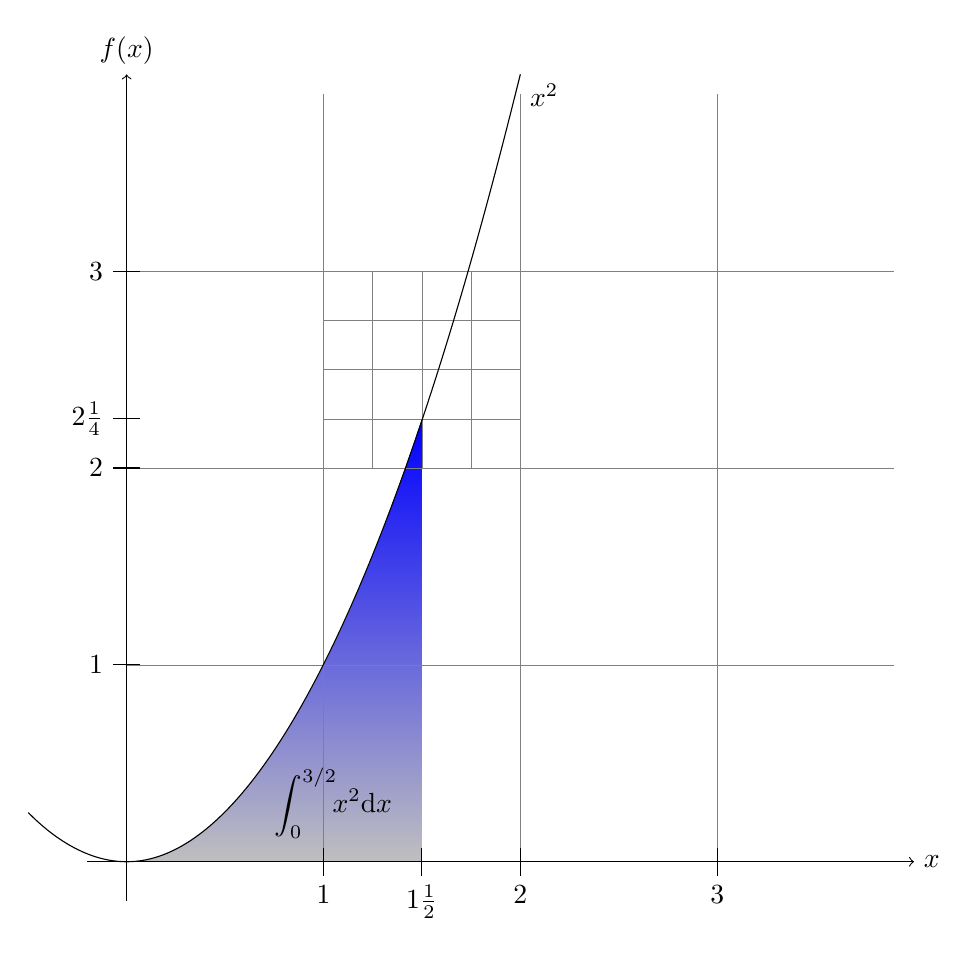
\begin{tikzpicture}[scale=2.5]
  \shade[top color=blue,bottom color=gray!50] 
      (0,0) parabola (1.5,2.25) |- (0,0);
  \draw (1.05cm,2pt) node[above] 
      {$\displaystyle\int_0^{3/2} \!\!x^2\mathrm{d}x$};

  \draw[style=help lines] (0,0) grid (3.9,3.9)
       [step=0.25cm]      (1,2) grid +(1,1);

  \draw[->] (-0.2,0) -- (4,0) node[right] {$x$};
  \draw[->] (0,-0.2) -- (0,4) node[above] {$f(x)$};

  \foreach \x/\xtext in {1/1, 1.5/1\frac{1}{2}, 2/2, 3/3}
    \draw[shift={(\x,0)}] (0pt,2pt) -- (0pt,-2pt) node[below] {$\xtext$};

  \foreach \y/\ytext in {1/1, 2/2, 2.25/2\frac{1}{4}, 3/3}
    \draw[shift={(0,\y)}] (2pt,0pt) -- (-2pt,0pt) node[left] {$\ytext$};

  \draw (-.5,.25) parabola bend (0,0) (2,4) node[below right] {$x^2$};
\end{tikzpicture}
\caption{یک نمودار زیبا با ارقام فارسی و قابلیت بزرگ‌نمایی بسیار، بدون از دست دادن کیفیت.}
\label{fig:parabola}
\end{figure}

\section{نحوه قرارگیری اشیای شناور}
\label{sec:floatObjs}
شکل‌ها، جداول و الگوریتم‌ها در لاتک اشیای شناور محسوب می‌شوند؛ یعنی خود لاتک تصمیم می‌گیرد آنها را در کجای صفحه ترسیم کند تا زیباتر باشد. اما می‌توان به لاتک توصیه کرد که آن را در قسمت خاصی از صفحه رسم کند. برای اینکه قاعدهٔ «ارجاع به جلو» رعایت شود باید فقط از پرچم
\verb|[ht]|
استفاده کرد، که می‌گوید اگر جا شد شکل را دقیقاً در همین مکان و در غیراینصورت در بالای صفحه بعد رسم کن.
بنابراین دستورات درج تصویر، جدول و الگوریتم به صورت زیر باید باشند:

\begin{latin}
\begin{verbatim}
	\begin{figure/table/algorithm}[ht]
		...
	\end{figure/table/algorithm}
\end{verbatim}
\end{latin}		% پیوست دوم: جدول، نمودار و الگوریتم در لاتک
% !TeX root=../main.tex
\chapter{مراجع، واژه‌نامه و حاشیه‌نویسی}
\label{app:refMan}
%\thispagestyle{empty}

\section{مراجع و نقل‌قول‌ها}
\label{sec:refUsage}
منابعِ پایان‌نامه، پایه و اساس تحقیق شما به حساب می‌آیند و ضرورت انجام مطالعه و روش‌های به کار رفته در بسیاری از قسمت‌های آن، به کمک منابع صورت می‌گیرد. در استفاده از مراجع علمی در پایان‌نامه، باید سعی کنید بیشتر از
\textbf{منابع چاپ‌شده و مهم}
استفاده کنید و
\emph{ارجاع به داده‌های چاپ نشده، خلاصه‌ها و پایان‌نامه‌ها، سبب به‌هم‌خوردگی و کاهش اعتبار قسمت ارجاع منابع می‌شود.}
استفاده از منابع و نقل قول‌هایی به تحقیق شما ارزش می‌دهند که
\textbf{در راستای هدف تحقیق بوده و به آن اعتبار ببخشند.}
برخی از دانش‌جویان تصوّر می‌کنند که کثرت نقل‌قول‌ها و ارجاعات زیاد، مهم‌ترین معیار علمی شدن پایان‌نامه است؛ حال آنکه استناد به تعداد کثیری از منابع بدون مطالعه دقیق آنها و استفادهٔ مستقیم در پایان‌نامه، می‌تواند نشان‌دهندهٔ عدم احساس امنیت نویسنده باشد!

دو روش برای استفاده از نتایج، جملات، داده‌ها و روش‌های دیگران وجود دارد. یکی نقل‌قول مستقیم و دقیق است و دیگری استفاده غیرمستقیم در متن مقاله، که در ادامه به قواعد این دو نوع نقل‌قول و ارجاع‌دهی اشاره می‌کنیم:
\begin{description}
	\item[نقل‌قول مستقیم:]
	نقل‌قول مستقیم باید دقیق و بدون هیچ تغییری در جملات باشد. بهتر است این‌گونه نقل‌قول‌ها تا حد امکان کوتاه باشد. جملات کوتاه داخل گیومه قرار می‌گیرند و باید به منبع دقیق آن، طبق روش ارجاع‌دهی به منابع، اشاره شود. به عنوان مثال در
	\cite{persianbib87userguide}
	آمده است که:
	\begin{quote}
		«با استفاده از فیلد
		\lr{AUTHORFA}
		می‌توان معادل فارسی نام نویسندگان مقالات لاتین را در متن داشت. معمولاً در اسناد فارسی خواسته می‌شود که پس از ذکر معادل فارسی نام نویسنده، نام لاتین نویسنده(ها) به عنوان پاورقی درج شود
		\citep{persianbib87userguide}.»
	\end{quote}
	\item[نقل‌قول غیرمستقیم:]
	نقل‌قول غیرمستقیم به معنی استفاده از ایده‌ها، نتایج، روش‌ها و داده‌های دیگران در درون متنِ پایان‌نامه، ولی به سبک خودتان و متناسب و هماهنگ با روند پایان‌نامهٔ شماست. در این حالت نیز باید متناسب با شیوهٔ ارجاع‌دهی به آن استناد شود.
\end{description}

با توجه به وجود سبک‌های مختلف ارجاع‌دهی، باید
\textbf{روش قابل قبول و یکسانی}
در طول پایان‌نامه برای اشاره به مراجع در متن و همچنین تهیه فهرست مراجع در انتهای پایان‌نامه بکار رود. مثلاً برای پایان‌نامه‌های مهندسی می‌توان از سبک ارجاع‌دهی
\lr{IEEE}%
\LTRfootnote{\url{http://www.ieee.org/documents/ieeecitationref.pdf}}
یا
\lr{acm}
استفاده کرد. طبیعتاً باید تناظر یک‌به‌یک بین فهرست مراجع در انتهای گزارش و مراجع مورد استفاده در متن باشد%
\footnote{البته گاهی ممکن است محقق مرجعی را مورد مطالعه قرار داده لیکن در متن به آن اشاره نکرده باشد؛ برخی معتقدند در این موارد نیز آوردن آن در فهرست مراجع، اشکالی ندارد، به این شرط که از عنوان «فهرست منابع» به جای «فهرست مراجع» استفاده شود.}.

برای سهولت مدیریت مراجعِ \پ%
، اکیداً توصیه می‌شود از یک ابزار «مدیریت منابع» (با خروجی
\texorpdfstring{\lr{Bib\TeX}}{Bib\TeX}%
) همچون
\lr{Mendeley}،
\lr{Zotero},
\lr{EndNote}
یا
\lr{Citavi}
استفاده کنید.

\subsection{ مدیریت مراجع با  \texorpdfstring{\lr{Bib\TeX}}{Bib\TeX}}
در بخش \ref{Sec:Ref} اشاره شد که با دستور 
 \lr{\textbackslash bibitem}
  می‌توان یک مرجع را تعریف نمود و با فرمان
 \lr{\textbackslash cite}
  به آن ارجاع داد. این روش برای تعداد مراجع زیاد و تغییرات آنها مناسب نیست. برای مدیریت منابع زیاد، سه بستهٔ
\lr{BibTeX} (پیش‌فرض),
\lr{natbib}
(ارجاع‌دهی در متن به صورت نویسنده-سال)
و \lr{BibLaTeX} (جدید و منعطف‌پذیر)
وجود دارند. در ادامه توضیحاتی در مورد مدیریت منابع با \lr{BibTeX} و \lr{natbib} در زی‌پرشین خواهیم آورد که همراه با توزیع‌های معروف تِک عرضه می‌شوند
\footnote{روش \lr{BibLaTeX} هنوز برای متون فارسی به درستی ترجمه نشده است.}.

یکی از روش‌های قدرتمند و انعطاف‌پذیر برای نوشتن مراجعِ مقالات و مدیریت مراجع در لاتک، استفاده از  \lr{BibTeX} است.
 روش کار با بیب‌تک به این صورت است که مجموعهٔ همهٔ مراجعی را که در \پ استفاده کرده یا خواهیم کرد، 
در پروندهٔ جداگانه‌ای با پسوند
\lr{bib}
نوشته و به آن فایل در سند خودمان به صورت مناسب لینک می‌دهیم.
 کنفرانس‌ها یا مجله‌های گوناگون برای نوشتن مراجع، قالب‌ها یا قراردادهای متفاوتی دارند که به آنها استیل‌های مراجع گفته می‌شود.
 در این حالت به کمک ‌استیل‌های بیب‌تک خواهید توانست تنها با تغییر یک پارامتر در پروندهٔ ورودی خود، مراجع را مطابق قالب موردنظر تنظیم کنید. 
 بیشتر مجلات و کنفرانس‌های معتبر یک فایل سبک
 (\lr{BibTeX Style})
با پسوند \lr{bst} در وب‌گاه خود می‌گذارند که برای همین منظور طراحی شده است.

به جز نوشتن مقالات، این سبک‌ها کمک بسیار خوبی برای تهیهٔ مستندات علمی همچون پایان‌نامه‌هاست که فرد می‌تواند هر قسمت از کارش را که نوشت مراجع مربوطه را به بانک مراجع خود اضافه نماید. با داشتن چنین بانکی از مراجع، وی خواهد توانست به راحتی یک یا چند ارجاع به مراجع و یا یک یا چند بخش را حذف یا اضافه ‌نماید؛ 
مراجع به صورت خودکار مرتب شده و
\textbf{فقط مراجع ارجاع داده شده در قسمت کتاب‌نامه خواهندآمد.}
قالب مراجع به صورت یکدست مطابق سبک داده شده بوده و نیازی نیست که کاربر درگیر قالب‌دهی به مراجع باشد. 

\subsection{سبک‌های مورد تأیید دانشگاه تهران}
طبق «دستورالعمل نگارش و تدوین پایان‌نامه» دانشگاه تهران در
\cite{UTThesisGuide}،
ارجاع در متن می‌تواند مطابق با هر یک از دو الگوی هاروارد یا ونکوور باشد:
\singlespacing
\begin{description}
	\item[سیستم نویسنده-سال (هاروارد):]
	ذکر نام نویسنده و سال نشر در متن. در این الگو مراجع بر اساس حروف الفبا تنظیم می‌گردند.
	\item[سیستم شماره‌دار (ونکوور):]
	ارجاع به مراجع به کمک شماره در متن. در این الگو شماره هر مرجع به ترتیب ظاهر شدن آن در متن در داخل کروشه قرار می‌گیرد. فهرست مراجع نیز بر اساس شماره مرجع (نه حروف الفبا) تنظیم می‌گردد.
\end{description}
\doublespacing

در مدیریت منابع با
\lr{\textbf{BibTeX}}،
ارجاع‌ها در متن تنها به شکل
\textbf{شماره‌دار (ونکوور)}
امکان‌پذیر است، گرچه فهرست مراجع می‌تواند با روش‌های مختلف مرتب شود. اگر بخواهیم ارجاع‌ها در متن به صورت
\textbf{نویسنده-سال (هاروارد)}
باشد باید از بستهٔ
\lr{\textbf{natbib}}\LTRfootnote{Natural Sciences Citations \& References}
و استیل‌های مختلف آن استفاده کنیم.

هنگام استفاده از روش نویسنده-سال نوع پرانتزگذاری‌ها در وسط و انتهای جمله با هم فرق خواهد داشت. به مثال زیر مطابق با دستورالعمل
\cite{UTThesisGuide}
توجه کنید:

\textit{
ابتدا
\cite{Khalighi87xepersian}
بستهٔ زی‌پرشین را برای حروف‌چینی فارسی اختراع کرد. بعدها سبک‌های ارجاع‌دهی فارسی و قالب‌های پایان‌نامه نیز مبتنی بر آن ساخته شد
\citep{persianbib87userguide}.
ارجاع‌دهی به مراجع لاتین نیز در زی‌پرشین امکان‌پذیر است. مثلاً
\citelatin{Gonzalez02book}
یک کتاب انگلیسی است و به راحتی به مقالات انگلیسی نیز می‌توان ارجاع داد
\citeplatin{kim2016integrated}.}

در این مثال، ۴ ارجاع در وسط و انتهای جمله به مراجع فارسی و انگلیسی آمده است. وقتی از سیستم نویسنده-سال استفاده می‌کنید، بهتر است ارجاع‌های آخر جمله کلاً داخل پرانتر بیاید؛ بدین منظور باید به جای
\verb|\cite|
از
\verb|\citep|
استفاده کنید. اما در سیستم شماره‌دار چون تمام ارجاع‌ها داخل کروشه می‌آیند این امر اهمیت ندارد.\\
نمی‌توانید در متن فارسی، اسم لاتین محقق خارجی را بیاورید و برای جلوگیری از ایجاد ابهام، صرف‌نظر از نام لاتین هم مجاز نیست! توصیه می‌شود که نام محقق خارجی در متن با حروف فارسی و در پاورقی اسم تمام نویسندگان به صورت انگلیسی آورده شود. نحوهٔ رعایت این نکته را می‌توانید در کد مثال بالا ببینید.

گرچه در تمپلت ورد
\cite{UTThesisGuide}،
به صراحت ذکر شده که بهتر است برای پایان‌نامه‌های مهندسی از سبک 
\lr{IEEE}
استفاده شود (که از سیستم ونکوور تبعیت می‌کند)، اما ترتیب فهرست مراجع در
\lr{IEEE}
بر اساس ترتیب ارجاع در متن بوده و
\emph{مراجع انگلیسی و فارسی از هم تفکیک نمی‌شوند}
که متضاد با دستورالعمل
\cite{UTThesisGuide}
و نیز متضاد عرف اکثر پایان‌نامه‌های فارسی است.
بنابراین دقیقاً نمی‌توان سبک خاصی را برای مراجع پایان‌نامه‌های دانشگاه تهران اجبار کرد. مهم این است که
\textbf{سبک ارجاع‌دهی در تمام طول یک کتابچه}
(مثلاً پایان‌نامه، مقالات یک مجله یا کل یک کتاب) یکسان باشد. بهتر است
\textbf{بسته به حوزه پایان‌نامه}،
در این مورد با استاد راهنمای خود مشورت کنید.

\subsection{سبک‌های فارسی قابل استفاده در زی‌پرشین}
تعدادی از سبک‌های فارسی بسته
\lr{Persian-bib}%
\footnote{ برای اطلاع بیشتر به راهنمای بستهٔ
\lr{Persian-bib}
مراجعه فرمایید.}
که برای  زی‌پرشین آماده شده‌اند، عبارتند از:

\singlespacing
\begin{itemize}
\item \emph{سبک‌های شماره‌دار}:
	\begin{description}
	\item [unsrt-fa.bst] این سبک متناظر با \lr{unsrt.bst} می‌باشد. مراجع به ترتیب ارجاع در متن ظاهر می‌شوند.
	\item [plain-fa.bst] این سبک متناظر با \lr{plain.bst} می‌باشد. مراجع بر اساس نام‌خانوادگی نویسندگان، به ترتیب صعودی مرتب می‌شوند.
	 همچنین ابتدا مراجع فارسی و سپس مراجع انگلیسی خواهند آمد.
	\item [acm-fa.bst] این سبک متناظر با \lr{acm.bst} می‌باشد. شبیه \lr{plain-fa.bst} است.  قالب مراجع کمی متفاوت است. اسامی نویسندگان انگلیسی با حروف بزرگ انگلیسی نمایش داده می‌شوند. (مراجع مرتب می‌شوند)
	\item [ieeetr-fa.bst] این سبک متناظر با \lr{ieeetr.bst} می‌باشد. (مراجع مرتب نمی‌شوند)
	\end{description}
	
\item \emph{سبک‌های نویسنده-سال}:
	\begin{description}
	\item [plainnat-fa.bst] این سبک متناظر با \lr{plainnat.bst} می‌باشد. نیاز به بستهٔ \lr{natbib} دارد. (مراجع مرتب می‌شوند)
	\item [chicago-fa.bst] این سبک متناظر با \lr{chicago.bst} می‌باشد. نیاز به بستهٔ \lr{natbib} دارد. (مراجع مرتب می‌شوند)
	\item [asa-fa.bst] این سبک متناظر با \lr{asa.bst} می‌باشد. نیاز به بستهٔ \lr{natbib} دارد. (مراجع مرتب می‌شوند)
	\end{description}
\end{itemize}
\doublespacing

با استفاده از استیل‌های فوق می‌توانید به انواع مختلفی از مراجع فارسی و لاتین ارجاع دهید.
به عنوان مثال‌هایی از
\textbf{مراجع انگلیسی}،
مرجع
\cite{Baker02limits}\footnote{چون فیلد \lr{authorfa} برای این مرجع تعریف نشده در سبک نویسنده-سال با حروف لاتین به آن در متن ارجاع می‌شود که غلط است.}
مقالهٔ یک ژورنال، مرجع
\cite{Amintoosi09video}
مقالهٔ یک کنفرانس، مرجع
\citelatin{Gonzalez02book}
یک کتاب، مرجع
\cite{Khalighi07MscThesis}
پایان‌نامهٔ کارشناسی ارشد و مرجع
\citelatin{Borman04thesis}
یک رسالهٔ دکتری می‌باشد.\\
همچنین در میان
\textbf{مراجع فارسی},
مرجع
\cite{Vahedi87}
مقالهٔ یک مجله، مرجع
\cite{Amintoosi87afzayesh}
مقالهٔ یک کنفرانس، مرجع
\cite{Pedram80osool}
یک کتاب ترجمه‌شده با ذکر مترجمان و ویراستاران، مرجع
\cite{Pourmousa88mscThesis}
پایان‌نامهٔ کارشناسی ارشد%
\footnote{همان‌طور که در بخش
\ref{sec:refUsage}
اشاره شد، بهتر است زیاد از پایان‌نامه‌ها در مراجع استفاده نکنید.}،
مرجع
\cite{Omidali82phdThesis}
یک رسالهٔ دکتری و مراجع
\cite{persianbib87userguide, Khalighi87xepersian}
نمونه‌های متفرقه هستند.

\subsection{ساختار فایل مراجع}
برای استفاده از بیب‌تک باید مراجع خود را در یک فایل با پسوند \lr{bib} ذخیره نمایید. یک فایل \lr{bib} در واقع یک پایگاه داده از مراجع%
\LTRfootnote{Bibliography Database}
شماست که هر مرجع در آن به عنوان یک رکورد از این پایگاه داده
با قالبی خاص ذخیره می‌شود. به هر رکورد یک مدخل%
\LTRfootnote{Entry}
گفته می‌شود. یک نمونه مدخل برای معرفی کتاب \lr{Digital Image Processing} در ادامه آمده است:

\singlespacing
\begin{LTR}
\begin{verbatim}
@BOOK{Gonzalez02image,
  AUTHOR     = {Gonzalez,, Rafael C. and Woods,, Richard E.},
  TITLE      = {Digital Image Processing},
  PUBLISHER  = {Prentice-Hall, Inc.},
  YEAR       = {2006},
  ISBN       = {013168728X},
  EDITION    = {3rd},
  ADDRESS    = {Upper Saddle River, NJ, USA}
}
\end{verbatim}
\end{LTR}
\doublespacing

در مثال فوق، \lr{@BOOK} مشخصهٔ شروع یک مدخل مربوط به یک کتاب و \lr{Gonzalez02book} برچسبی است که به این مرجع منتسب شده است.
 این برچسب بایستی یکتا باشد. برای آنکه بتوان
\textbf{برچسب مراجع}
 را به راحتی به خاطر سپرد و حتی‌الامکان برچسب‌ها متفاوت با هم باشند، معمولاً از قوانین خاصی به این منظور استفاده می‌شود. یک قانون می‌تواند
\textbf{فامیل نویسنده اول + دورقم سال نشر + اولین کلمهٔ عنوان اثر}
باشد. به
\lr{AUTHOR}، \lr{TITLE}، $\dots$ و \lr{ADDRESS}
فیلدهای این مدخل گفته می‌شود، که هر یک با مقادیر مربوط به مرجع پر شده‌اند. ترتیب فیلدها مهم نیست. 

انواع متنوعی از مدخل‌ها برای اقسام مختلف مراجع همچون کتاب، مقالهٔ کنفرانس و مقالهٔ ژورنال وجود دارد که برخی فیلدهای آنها با هم متفاوت است. 
نام فیلدها بیانگر نوع اطلاعات آن می‌باشد. مثالهای ذکر شده در فایل \lr{MyReferences.bib} کمک خوبی برای شما خواهد بود. 
%این فایل یک فایل متنی بوده و با ویرایشگرهای معمول همچون \lr{Notepad++} قابل ویرایش می‌باشد. برنامه‌هایی همچون 
%\lr{TeXMaker}
% امکاناتی برای نوشتن این مدخل‌ها دارند و به صورت خودکار فیلدهای مربوطه را در فایل \lr{bib}  شما قرار می‌دهند.  
با استفاده از سبک‌های فارسی آماده شده، محتویات هر فیلد می‌تواند به فارسی نوشته شود؛ ترتیب مراجع و نحوهٔ چینش فیلدهای هر مرجع را سبک مورد استفاده  مشخص خواهد کرد.

\textbf{در فایل 
\lr{MyReferences.bib}
 که همراه با این \پ هست، مثال‌های مختلفی از مراجع آمده‌اند که برای درج مراجع خود، تنها کافیست مراجع‌تان را جایگزین موارد مندرج در آن نمایید.
}

برای بسیاری از مقالات لاتین حتی لازم نیست که مدخل مربوط به آنرا خودتان بنویسید. با جستجوی 
\textbf{نام مقاله + کلمه
\lr{bibtex}}
در اینترنت سایت‌های بسیاری همچون
\lr{ACM} و \lr{ScienceDirect}
را خواهید یافت که مدخل
\lr{bibtex}
مربوط به مقاله شما را دارند و کافیست آنرا به انتهای فایل
\lr{MyReferences.bib}
اضافه کنید.

\subsection{نحوه اجرای \texorpdfstring{\lr{Bib\TeX}}{Bib\TeX}}
پس از قرار دادن مراجع خود، برای ساخت فایل خروجی می‌توانید دستور زیر را (در ترمینال یا از طریق \lr{Texmaker}) اجرا کنید:%
\footnote{فایل \lr{latexmkrc} باید در کنار \lr{main.tex} وجود داشته باشد.}

\singlespacing
\begin{LTR}
	\begin{verbatim}
		latexmk -bibtex -pdf main.tex
	\end{verbatim}
\end{LTR}
\doublespacing
ابزار \lr{latexmk} مراحل مختلف ساخت خروجی لاتک را به طور خودکار و بهینه انجام می‌دهد و هر بار فقط مراحلی را که لازم باشد تکرار می‌کند.
روش دستی‌تر این است که یک بار \lr{XeLaTeX} را روی سند خود اجرا نمایید، سپس \lr{bibtex} و پس از آن هم ۲ بار \lr{XeLaTeX} را. در \lr{TeXMaker} کلید \lr{F11} و در \lr{TeXWorks} هم گزینه‌ی \lr{BibTeX} از منوی \lr{Typeset}، \lr{BibTeX} را روی سند شما اجرا می‌کنند.

\section{واژه‌نامه‌ها و فهرست اختصارات}
\gls{Gloss}
یا فرهنگ لغات، مجموعه‌ای از اصطلاحات و تعاریف خاص و فنی است که معمولاً در انتهای یک کتاب می‌آید. چون پایان‌نامه خود یک متن تخصصی بلند محسوب می‌شود، استفاده از فرهنگ لغات در انتهای آن به شدت توصیه می‌شود، خصوصاً که احتمال استفاده از لغات تخصصی لاتین در آن بالاست.
واژه‌نامه‌هایی که در انتهای کتاب‌های انگلیسی می‌آیند معمولاً تک‌زبانه هستند و معنی یک اصطلاح تخصصی در آنها، عمدتاً به صورت یک
\gls{Description}
طولانی آورده می‌شود. اما چون در متون فارسی، آوردن لغات انگلیسی مجاز نیست و باید معادل فارسی آنها وارد شود، جهت رفع ابهام معمولاً واژه‌نامهٔ فارسی به انگلیسی (و برعکس) در انتهای کتاب درج شده و  
\glspl{Description}
در صورت نیاز در متن آورده می‌شوند.

فهرست
\glspl{Acronym}
شامل نمادهای کوتاهی است که اغلب از حروف ابتدایی کلمات یک عبارت طولانی ساخته شده‌اند. با اینکه
\glspl{Acronym}
با حروف (بزرگ) لاتین نوشته می‌شوند، اما چون کوتاهند استفاده از آنها در میان متن فارسی مجاز است. با این حال برای رفع ابهام، عرف است که فهرستی از آنها شامل معنی هر نماد، در کنار دیگر فهرست‌ها در ابتدای متن درج شود.

در این قالب پایان‌نامه، برای ساخت و مدیریت واژه‌نامه و فهرست اختصارات از بستهٔ پیشرفتهٔ
\lr{glossaries}
با موتور واژه‌نامه‌سازی
\lr{xindy}
استفاده می‌شود. تنظیمات بهینهٔ این بسته در فایل
\lr{glossaries-settings.tex}
عبارتند از:
\begin{itemize}
	\item
قبل از درج واژه‌ها در متن، باید مدخل آنها با دستور زیر (ترجیحاً در فایل جدای \lr{words.tex}) تعریف شود:
	\begin{LTR}
	\verb|\newword{Label}{Word}|\{واژه\}\{واژه‌ها\}
	\end{LTR}
	
	\item
قبل از وارد کردن علائم اختصاری در متن، باید مدخل آنها نیز (ترجیحاً در فایل \lr{acronyms.tex}) به صورت زیر تعریف شود:
	\begin{LTR}
	\verb|\newacronym{Label}{Acr}|\{معنی‌اختصار\}
	\end{LTR}

	\item
جهت درج یک علامت اختصاری یا معادل یک واژه تخصصی، کافی است از دستور
	\verb|gls{Label}|
در متن استفاده کنید. دستور
	\verb|glspl{Label}|
نیز برای آوردن معادل یک لغت در حالت جمع ساخته شده است.
	
	\item
هنگام اولین استفاده از یک معادل فارسی یا اختصار در متن، معادل انگلیسی یا معنی آن در پاورقی آورده می‌شود. در صورتی که هر یک از این پیش‌فرض‌ها را دوست ندارید با ویرایش فایل
	\lr{glossaries-settings.tex}
می‌توانید آن را تغییر دهید.

	\item
در انتهای پایان‌نامه با دستور
\verb|\printglossary|
فهرست کلمات استفاده‌شده به ترتیب الفبای فارسی (واژه‌نامه فارسی به انگلیسی) و الفبای انگلیسی (واژه‌نامه انگلیسی به فارسی) درج می‌شود.
\end{itemize}

به عنوان مثال، با مشاهدهٔ کد این نوشته، نحوهٔ درج معادل فارسی
\gls{RandomVariable}
را در متن مشاهده می‌کنید.
در نمایش واژهٔ
\gls{RandomVariable}
برای بار دوم، معادل لاتین در پاورقی نمی‌آید.
در مورد درج علائم اختصاری، مثلاً می‌توان به رابطهٔ
\gls{F}
اشاره کرد.

\section{حاشیه‌نویسی در نسخه پیش‌نویس}
اصلاح و بازبینی چندین و چندبارهٔ یک پایان‌نامه یا مقاله، از معمول‌ترین امور در نگارش آن می‌باشد. فرض کنید دانشجو پایان‌نامه یا مقالهٔ خود را (کامل یا ناقص) نوشته و می‌خواهد نظر استاد راهنما، اعضای آزمایشگاه یا دیگر متخصصین را در مورد آن جویا شود. به جز مشاورهٔ حضوری، تلفنی یا از طریق ایمیل، برای اظهارنظر دقیق بر نوشته، می‌توان از ابزارهای حاشیه‌نویسی در فایل
\lr{PDF}
یا \lr{tex}
نیز استفاده کرد.

یک راهکار مناسب برای حاشیه‌نویسی در فایل \lr{tex}، استفاده از بسته 
\lr{todonotes}
می‌باشد که آقای خلیقی به تازگی امکان استفاده از آن را برای فارسی‌زبانان نیز فراهم آورده‌اند.
بدین منظور، هر جایی که خواستید نکته یا نکاتی را در حاشیه متن یادداشت کنید، کافی است دستور زیر را وارد نمایید:
\begin{latin}
\verb|\todo{NOTE}|
\end{latin}
مثلاً استاد راهنما می‌تواند از دانشجو بخواهد که در بخشی توضیح بیشتری دهد.
\todo{
توضیح بیشتری لازم است.
}
استاد راهنما یا داور حتی می‌تواند محل پیشنهادی برای درج یک تصویر را نیز به راحتی برای دانشجو مشخص کند.
\missingfigure[figwidth=\textwidth,figcolor=white]{یک تصویر از خروجی الگوریتم 
\ref{alg:RANSAC}
را در اینجا قرار دهید.}
یکی دیگر از امکانات این بسته آن است که می‌توان فهرست نکات را در ابتدای سند داشت. بسته 
\lr{todonotes}
امکانات بسیاری دارد
\todo[fancyline,color=green!30]{مرجع این مطلب؟}
که در راهنمای آن معرفی شده است و با اجرای دستور زیر در خط فرمان می‌توانید آنها را مشاهده کنید:
\begin{latin}	
	\texttt{texdoc todonotes}
\end{latin}	
دقت کنید که توضیحات حاشیه‌ای و فهرست کارهای باقیمانده (نکات)،
\textbf{فقط در نسخه
\gls{Draft}}
قابل دیدن هستند و در نسخه نهایی، نمایش داده نخواهند شد.
برای استفاده از حالت
\gls{Draft}
باید گزینه 
\lr{draft}
به دستور 
\verb|\documentclass|
در ابتدای فایل 
\lr{main.tex}
اضافه شود.
هنگامی‌که سند شما در حالت 
\gls{Draft}
باشد:

\singlespacing
\begin{enumerate}
\item 
هیچ یک از صفحات آغازین پایان‌نامه، تا فهرست مطالب نمایش داده نمی‌شود (به جز صفحه اول).
\item
روی صفحه اول عبارت «پیش‌نویس» به صورت درشت و کم‌رنگ نمایش داده می‌شود.
\item
فهرست نکات درج شده توسط
\lr{todo}،
پس از فهرست اصلی و با عنوان «فهرست کارهای باقیمانده» نمایش داده می‌شود.
\item
شماره صفحاتی که به هر مرجع ارجاع داده شده است در بخش مراجع نمایش داده می‌شود
\footnote{اعمال گزینهٔ
\lr{pagebackref}
برای بستهٔ
\lr{hyperref}.
}.
\end{enumerate}
\doublespacing
هر یک از موارد بالا تا زمانی که نسخه نهایی \پ نیاز نباشد بسیار مورد توجه و مفید واقع می‌شوند.
   	% پیوست سوم: مراجع، واژه‌نامه و حاشیه‌نویسی

% برگرداندن شماره‌بندی صفحات فصول
\let\chapter\Chapter
\pagenumbering{tartibi} % اول، دوم، ...
%\baselineskip=.75cm

% چاپ واژه‌نامه‌ها و نمایه 
\onehalfspacing
\printglossary
\printindex

\begin{latin}
\baselineskip=.6cm
\latinTitlePage
\end{latin}
\label{LastPage}

\end{document}